%%%%%%%%%%%%%%%%%%%%%%%%%%%%%%%%%%%%%%%%%%%%%%%%%%%%%%%%%%%%%%%%%%%%%%%%%%%%%%%%%%%%%%%%%%%
%%
%% The updated version of this document should be downloaded from
%%      https://github.com/jp-um/university_of_malta_LaTeX_dissertation_template
%%
%% In case of any difficulties please contact Dr JP Ebejer on jean.p.ebejer@um.edu.mt
%%
%%%%%%%%%%%%%%%%%%%%%%%%%%%%%%%%%%%%%%%%%%%%%%%%%%%%%%%%%%%%%%%%%%%%%%%%%%%%%%%%%%%%%%%%%%%

%% Before you embark on this quest you should probably read some of:
%% Deadly sins - http://ctan.mirror.garr.it/mirrors/CTAN/info/l2tabu/english/l2tabuen.pdf
%% Writing a thesis in LaTeX - http://tug.org/pracjourn/2008-1/mori/mori.pdf

\RequirePackage[l2tabu, orthodox]{nag} % tells you of any bad LaTeX usage
                                       % must be first thing in class (with the exception of comments)

%% There is one option you should define; oneside or twoside
%% Use twoside for your viva docs (examiners hate long docs they need to carry around)
%% and oneside for the final thing you submit to the library.  Note that margins will
%% change accordingly

%\documentclass[twoside]{um}  % custom University of Malta project/dissertation/thesis 
\documentclass[oneside]{um}

%% **************** (Your) Packages (Start) ******************

% \listfiles % uncomment this to know which packages you are using
              % the list of packages will be in the bottom of the .log file

%% Note that packges may already be loaded from the um (and memoir) classes.
%% Do not add your packages to the template, but rather add them here.

\usepackage{blindtext} %% for some dummy text, remove in your writeup
\usepackage{coffee4}    %% for some fun
\usepackage{amsmath}
\usepackage{xcolor}
\usepackage{placeins}
\usepackage{algorithm}
\usepackage{algpseudocode}
\usepackage[utf8]{inputenc}
\usepackage{booktabs}
\usepackage{tabularx}
\usepackage{geometry}
\usepackage{rotating}
\usepackage{pdflscape}
\usepackage{pgfgantt}
\usepackage{xcolor}
\usepackage{tabularx}
\usepackage{wrapfig}
\usepackage{float}
\usepackage{enumitem}
\usepackage{caption}
\usepackage{subcaption}

%% ***************** (Your) Packages (End) *******************


%% **************** (Your) Data (Start) ******************



\title{End-to-End \\
Autonomous Navigation using Homography-Based Overhead Localization
}                                                   % use \\ here otherwise you get a justified title
                                                    % note capitalization of the title (only common 
                                                    % words in lower case) 

\makeatletter
\def\@tagline{}
\makeatother

\author{John Christian Niño T. Abuel \\
        Rey Iann Tigley\\
        Kervin Lemuel Paalisbo\\
        }                             

\supervisor{Renato V. Crisostomo}                 % your supervisor(s) name - no . in Dr
%\cosupervisor{Dr Who}                              % your cosupervisor(s) name - no . in Dr ** OPTIONAL ** 
                                                    % simply comment out the above line if absent
\department{Department of Computer Science}         % your department 
\faculty{College of Computer Studies}               % your faculty (e.g. ICT)
\degree{B.S. in Computer Science}                   % the degree you are reading
                                                    % note the \ after the dot, so not to consider it a fullstop
\doctype{undergraduate thesis}                      % the type of document (fyp, dissertation, thesis)
\degreedate{June, 2026 }                             % when did you submit -- officially after your corrections !

%%\subjectcode{ICS5200}                             % the study unit-code (currently not used)

%% ***************** (Your) Data (End) *******************


%% ******** (Your) Document Settings (Start) *************

% You should have an images directory in every chapX subdir
% NOTE:  Trailing / for subdirs is required.
\graphicspath{{./images/}{./chap1/images/}}   % Paths where to look for images, if defined "images" must always be there as it holds the images in-use by the template.

\makeindex

%% ********* (Your) Document Settings (End) **************

% DOCTOR'S (JP) ORDERS: MAKE SURE TO READ MY TWO BLOG ENTRIES WITH
% CONTENT AND LaTeX TIPS FOR YOUR WRITE-UP.  THESE ARE BASED ON  
% EXAMINER'S FEEDBACK
%
% URLS:
% https://bitsilla.com/blog/2019/03/content-tips-for-your-dissertation-or-project-write-up/
% https://bitsilla.com/blog/2019/01/latex-tips-for-your-dissertation-or-project-write-up/

\usepackage[none]{hyphenat}
\sloppy

\parskip 7.2pt

%\raggedright

% end the preamble and start the document

\begin{document}

\cleardoublepage
\thispagestyle{empty}


\begin{table}[H]
\centering
\renewcommand{\arraystretch}{1.5}

\resizebox{\textwidth}{!}{
\begin{tabular}{|c|p{2.3cm}|p{8.2cm}|p{3.8cm}|p{1.2cm}|p{2.2cm}|}
\hline
\textbf{Revision No.} &
\textbf{Panelist} &
\textbf{Details of Revision / Suggestion} &
\textbf{Section} &
\textbf{Page} &
\textbf{Signature} \\
\hline

1 &
Prof. Orven E. Llantos &
Added the client--server system architecture illustrating the relationship among the camera, client, and server. &
Section 3.3.1 (Methodology) &
38 &
\\
\hline

2 &
Prof. Orven E. Llantos &
Added the Pixel-to-Centimeter (Pixel-to-cm) conversion in the methodology. &
Section 3.4.2 (State Representation) &
36--37 &
\\
\hline

3 &
Assistant Prof. Liezil Daberao &
Corrected the confusion matrix by changing the heading from ``CTE'' to ``Heading Error (Degrees).'' &
Section 4.5 &
82 &
\\
\hline

4 &
Assistant Prof. Haroun Macalisang &
Added the names of the Computer Science alumni in the Acknowledgements section. &
Acknowledgements &
iii &
\\
\hline

5 &
Assistant Prof. Haroun Macalisang &
Added baseline images for each experimental baseline. &
Section 4.1 &
62--67 &
\\
\hline

\end{tabular}
}
\end{table}

\vspace{0.8cm}

\frontmatter 
    \maketitle
    \input{frontmatter/copyright}          %
    %\input{frontmatter/originality}       %
    \begin{acknowledgements}
The researchers would like to express their sincere gratitude and appreciation to the following individuals who donated computer units to support the department's Artificial Intelligence/Machine Learning training initiatives: 

\begin{center} 
\begin{tabular}{ll} 
\textbf{Mr. Christian Riconalla} & \textbf{Ms. Jamila Hojas} \\ 
\textbf{Mr. Julius Serino} & \textbf{Mr. Jan Ancajas} \\ 
\textbf{Ms. Maryland Sara} & \textbf{Mr. Jose "Pepe" Cueto} \\
\textbf{Ms. Kathrina Ondap} & \textbf{Mr. Clayde Bael} \\ 
\textbf{Mr. Jeremy Pinzon} & \textbf{Dr. Meriam Gay Bautista-Jurney} \\
\textbf{Mr. Erle Czar Mantos} & \textbf{Mr. Cris Tabanag} \\  
\textbf{Ms. Paula Rudman}
\end{tabular} 
\end{center} 

Their generosity has greatly enhanced the department's computing resources, providing students with the opportunity to gain practical experience in Artificial Intelligence, machine learning, and related technologies. These contributions will continue to support hands-on instruction, research, and project development, helping prepare Computer Science students for future careers in computing. 
The department sincerely thanks all of our donors for their invaluable support and commitment to advancing technology education.

The researchers would like to express their gratitude and appreciation to Asst Prof. Renato Crisostomo, our thesis adviser, for the invaluable guidance, insightful recommendations, patience, and continuous support throughout this research. Their expertise and encouragement were instrumental in the successful completion of this thesis.
The researchers are truly grateful for the time, knowledge, and effort generously shared during every stage of this work.
\end{acknowledgements} 
    %% For tips on how to write a great abstract, have a look at
%%	-	https://www.cdc.gov/stdconference/2018/How-to-Write-an-Abstract_v4.pdf (presentation, start here)
%%	-	https://users.ece.cmu.edu/~koopman/essays/abstract.html
%%	-	https://search.proquest.com/docview/1417403858
%%  - 	https://www.sciencedirect.com/science/article/pii/S037837821830402X

\begin{abstract}
Traditional autonomous navigation systems often rely on expensive sensors and computationally intensive algorithms, making them difficult to deploy on low-cost robotic platforms. This study proposes a lightweight end-to-end navigation framework that combines geometric computer vision and imitation learning for autonomous path following in structured indoor environments. Using a single RGB camera and ArUco fiducial markers, the system computes a homography matrix to transform camera images into a top-down Bird's-Eye-View (BEV) representation. These processed images are then fed into a lightweight Convolutional Neural Network (CNN) trained through behavioral cloning to directly predict steering commands.

The system was evaluated on four track topologies of increasing difficulty: 45-degree Bézier curves, a 90-degree square path, 180-degree U-turns, and a held-out track that was not seen during training. Performance was measured using cross-track error, heading error, and success rate across forty independent randomized-start trials. The controller successfully completed all trials without leaving the lane. On the unseen track, tracking error increased by only about 1.7 times compared to the trained tracks while maintaining a 100\% success rate, suggesting that the network learned transferable path geometry rather than memorizing specific routes. The complete system runs in real time on a Raspberry Pi, demonstrating that reliable autonomous navigation can be achieved using low-cost hardware and a single-camera setup. These results show that combining homography-based scene transformation with deep learning provides a practical alternative to more expensive SLAM-based navigation approaches in structured indoor environments.

Keywords: Autonomous Navigation, Convolutional Neural Networks, Homography, Behavioral Cloning, Mobile Robots, Computer Vision

\end{abstract}\if@openright\cleardoublepage\else\clearpage\fi
    \tableofcontents*\if@openright\cleardoublepage\else\clearpage\fi
    %\listoffigures*\if@openright\cleardoublepage\else\clearpage\fi
    %\listoftables*\if@openright\cleardoublepage\else\clearpage\fi
    %\input{frontmatter/abbreviations}\if@openright\cleardoublepage\else\clearpage\fi

%% Note: always use \input as you cannot nest \includes (amongst other things)
\pagestyle{umpage}
\mainmatter 
    \chapter{Introduction}

Autonomous navigation systems have traditionally been designed around the perspective of the moving robot itself. Cameras and sensors are mounted directly on the platform to capture a ground-level, ego-centric view of the environment, mirroring how a human driver perceives the road ahead. This design works well in environments where the navigation path is physically distinguishable: lane markings, boundary edges, or clear contrast between the drivable surface and its surroundings give the system enough visual information to follow a route. However, this fundamental assumption breaks down in a wide class of practical applications where no such ground path exists.

Consider autonomous lawn mowers operating across uniform grass, or robotic vacuum cleaners navigating featureless carpet and bare flooring. In these environments, the ground surface provides no inherent visual guidance given that there are no lane markings to follow, no edges to track, and no color contrast to exploit. Conventional ego-centric navigation approaches, including modern end-to-end deep learning systems trained to recognize road features, are architecturally unsuited to these conditions without significant redesign. A solution must be explored that does not depend on the robot's ability to see and recognize a physical ground path from its own perspective.

Beyond the absence of a visible path, existing autonomous navigation frameworks impose further constraints that limit their deployment in low-cost and resource-constrained settings. Existing solutions like Simultaneous Localization and Mapping (SLAM) rely on expensive sensor arrays like LiDAR, depth cameras, and inertial measurement units which is then paired with computationally intensive software pipelines that demand high-performance onboard processors. For compact consumer-grade platforms such as robotic vacuum cleaners and autonomous lawn mowers, these requirements are fundamentally mismatched with the operational realities of tight unit cost, limited power budgets, and minimal onboard processing capacity.

This study proposes an alternative navigation framework that addresses both of these constraints simultaneously. By separating path perception from the robot's onboard egocentric view, the system offloads visual processing to a fixed overhead camera and employs planar ArUco fiducial markers as geometric reference anchors. A homography transformation converts the overhead camera feed into a rectified top-down representation of the environment, and a lightweight Convolutional Neural Network trained through behavioral cloning maps this geometrically simplified visual input directly to continuous steering commands without any classical controller feedback, without expensive sensors, and without requiring a physically marked ground path. This establishes a foundational proof-of-concept for autonomous navigation in environments where the ground surface provides no inherent visual guidance, deployable on resource-constrained hardware.
\section{Background of the Study}

Autonomous navigation is the ability of robots and autonomous vehicles to generate a path and move along it without human intervention, utilizing data captured from onboard sensors and sometimes remote navigation aids \cite{Cebollada2020MobileRoboticsAI}. These systems consistently rely on simultaneous localization and mapping (SLAM) for autonomous navigation. Additionally, these systems also utilize LiDAR, depth cameras, or multi-sensor fusion \cite{Liu2024IndoorSensingReview, Wei2024SLAMResearchReview, Zhu2023CameraLidarIMUFusionSLAMSurvey}. While generally effective, these robotic systems demand high computational costs, expensive robotics components, and complex software integration requirements, which makes them less accessible for developing low-cost robotics platforms \cite{Chea2023CollaborativeConstructionRobot}. To address these limitations, previous studies have already explored computer-vision navigation using fiducial markers, which offer a simple, lightweight, and reliable framework for localization, particularly in structured environments \cite{Alghamdi2025MobileRobotMarkersMapping}.

According to \cite{kuzmenko2025fiducial}, a fiducial marker refers to a specialized code-type marker used in computer vision, which is set in an environment or scene to help imaging systems find reference points. The robustness of fiducial markers such as ArUco and AprilTag in providing low-cost localization has already been explored in a 2025 systematic review of the mapping of mobile robot navigation \cite{Alghamdi2025MobileRobotMarkersMapping}. The study of \cite{Mantha2022FiducialNetworkNavigation} concluded that marker size, spacing, and the placement of a fiducial marker may affect robot navigation, well-designed markers show potential in achieving high success rates with minimal computational overhead. 

Several recent studies probed the ability of ArUco markers to provide indoor localization for autonomous robot navigation. Research on planar indoor localization using ArUco \cite{Hinderer2025ArucoPlacementIndoor} and multi-marker setups illustrates that planar marker fields can deliver accurate 2-D pose estimates which are appropriate for autonomous robot navigation \cite{Lin2023MarkerBasedLocalization}, especially when combined with simple filters or odometry. To further maximize localization, multi-camera setups are also explored, as seen in the study of \cite{Sevgi2025MulticameraIndoorAruco}. Studies on fiducial‑marker networks for indoor navigation \cite{Braun2022RobotAtFactoryLocalization} explicitly frame markers as an alternative to the expensive SLAM for building service and inspection robots, highlighting low instrumentation and computation as key advantages.

For robot navigation, recent research has shown interest in using end-to-end frameworks that map visual input directly to steering \cite{Han2024NeuPAN} or obstacle avoidance actions, usually with deep reinforcement learning or attention-based architecture \cite{Zhou2025DRLSpatiotemporalTransformer, Yu2025RLAUVMotionSystems}. Although such methods can achieve strong obstacle avoidance performance in simulation or structured test environments, multiple studies emphasize issues with stability, overfitting, and susceptibility to noise, leading to poor generalization outside training conditions. 

Despite the demonstrated effectiveness of ArUco markers for localization and the growing body of work on end-to-end visual navigation, relatively few studies have explored combining these two domains. Most marker-based systems stop at pose estimation and hand off to classical controllers, while most end-to-end systems operate on raw ego-centric feeds without geometric preprocessing. This study addresses that intersection directly.

\section{Statement of the Problem} 
Current ego-centric, vision-based autonomous navigation models rely heavily on the presence of physical path features, such as lane markings, boundary edges, or distinct color contrasts between the drivable surface and its surroundings. When deployed in featureless environments such as uniform grass, carpet, or bare flooring, these foundational assumptions break down. Without a visually distinguishable ground path, conventional end-to-end deep learning approaches fail to generate reliable steering commands, rendering them fundamentally inapplicable to these environments without significant architectural redesign or the reliance on expensive, computationally heavy SLAM sensor arrays.

Conversely, while alternative localization methods using fiducial markers such as ArUco have proven effective for low-cost indoor tracking, existing marker-based systems predominantly hand off pose estimation or localization to classical control algorithms rather than utilizing neural network integration. There is a distinct gap in the literature regarding the intersection of fiducial marker localization and end-to-end imitation learning. Specifically, it remains unproven whether offloading visual perception to a fixed overhead camera and applying planar homography can simplify visual inputs sufficiently to allow a lightweight Convolutional Neural Network (CNN) to map those inputs directly to continuous steering commands, bypassing the need for classical controllers and physical ground paths entirely.

\section{Research Objective} 
The following are the general objective and specific objectives of the study.

\subsection{General Objective}
To develop an autonomous vehicle system with external top-down camera and utilizing an end-to-end Convolutional Neural Network (CNN) architecture that maps raw visual input, digitally augmented with a virtual ground path, directly to robot’s steering.
path.

\subsection{Specific Objectives}
\begin{enumerate}
    \item To implement a robust Inverse Perspective Mapping (IPM) pipeline using ArUco markers for dynamic homography calibration, capable of transforming angled, ego-centric RGB camera frames into rectified, top-down, bird’s-eye view (BEV) representations of the local path.
    \item To construct a specialized behavioral cloning dataset by manually driving the robot, consisting of synchronized pairs of preprocessed BEV path images and human-demonstrated steering angles, collected across various track configurations.
    \item To design and train a regression-based Convolutional Neural Network (CNN) architecture that maps high-dimensional BEV visual inputs directly to continuous steering commands (and optionally linear velocity), utilizing Mean Squared Error (MSE) loss for optimization.
    \item To deploy the trained model onto the robot's driving pipeline such that inference output is sent directly to the motor drivers, enabling fully autonomous navigation.
    \item To evaluate the autonomous robot by measuring lane‑keeping accuracy (CTE/RMSE), heading error, trial‑to‑trial consistency, and steering actuation behaviour, and summarizing results using confusion matrices and per‑scenario statistics.
\end{enumerate}

%\section{Proposed Solution} 

\section{Scope and Limitations of the Research}
This study focuses on the development of a low-cost, end-to-end autonomous navigation system using a single overhead RGB camera. The system utilizes Inverse Perspective Mapping (IPM) facilitated by ArUco markers to process visual inputs.

The hardware implementation is restricted to computationally constrained platforms (e.g., Raspberry Pi or NVIDIA Jetson Nano) to validate the lightweight nature of the proposed architecture. The robot operates exclusively in structured environments where ArUco markers can be reliably detected, and no 3-D mapping, LiDAR, or depth-based perception is included. Unlike traditional SLAM systems that integrate probabilistic mapping and multi-sensor fusion \cite{Cadena2016SLAMRobustPerception, Cieslewski2017DecentralizedVisualSLAM}, this study does not attempt full environment reconstruction or dynamic obstacle mapping. Instead, localization is constrained to planar marker fields consistent with research demonstrating accurate 2-D pose estimation using fiducials \cite{GarridoJurado2014FiducialMarkers, RomeroRamirez2018SpeededFiducialDetection}.

The study is also limited to a differential drive (2WD) chassis. This is intentional as the Convolutional Neural Network is not trained to output complex holonomic movements or deal with Ackermann steering physics.

As for the environmental scope of this study, the navigation environment is limited to structured, planar indoor surfaces with consistent artificial lighting. The robot operates within an area of interest, which is a predefined 2-D plane where ArUco markers are visible and explicitly placed to define track boundaries or reference points. The system is not designed for outdoor environments, uneven terrain, or varying illumination conditions.

Neural-network steering prediction is trained only on data collected within the experimental environment. Thus, the learned model is not expected to generalize to unstructured or markerless environments, consistent with known limitations of end-to-end visual navigation models regarding generalization and noise sensitivity \cite{Bansal2020ChauffeurNet, Codevilla2019BehaviorCloningLimits}. The evaluation metrics, cross-track accuracy, heading error, and success rate, are limited to controlled indoor trials and do not include long-term autonomy, multi-robot coordination, or obstacle-rich navigation.

\section{Significance of the Research } 
This study contributes to the growing demand for accessible and low cost autonomous driving robot navigation frameworks by presenting a system that removes the need for expensive sensors, advanced SLAM algorithms, and high-end computing hardware. While previous works have highlighted that fiducial markers such as Aruco provide efficient localization \cite{GarridoJurado2014FiducialMarkers, RomeroRamirez2018SpeededFiducialDetection}, relatively few studies have used these markers into a complete low cost 2-D navigation system suited for educational or research purposes.

This research contributes to the field of robotic control by exploring the potential of End-to-End Imitation Learning in constrained environments. While previous works have validated ArUco markers for localization \cite{RomeroRamirez2018SpeededFiducialDetection} and CNNs for visual navigation separately, this study bridges these domains. It investigates whether a homography-based pre-processing step can simplify visual inputs enough to allow a lightweight neural network to provide navigation controls accurately without the computational overhead of deeper, complex architectures.

The study is locally and globally significant because it provides:

\begin{enumerate}
    \item A framework for implementing advanced Deep Learning concepts using only a standard webcam and a microcontroller, making the technology accessible for educational and low-resource industrial applications.
    \item A simple experimental platform for teaching concepts related to localization, control systems, and machine learning.
    \item A replicable and scalable framework for researchers exploring low-cost autonomous navigation in structured indoor spaces.
\end{enumerate}

Overall, this study aims to address the gaps in the literature by producing a fully integrated, low-cost navigation framework that combines fiducial-marker localization and End-to-End robot control, offering a practical solution for accessible autonomous robot navigation systems.

%\blindtext
 
    \chapter{Literature Review}
\textbf{This chapter reviews the existing literature on autonomous mobile recognition systems, with a focus on sensor technologies, marker based localization, and robot control strategies. It analyzes the advantages and limitations of current methodologies to establish the theoretical framework for the proposed low-cost navigation system. Additionally, the Preferred Reporting Items for Systematic Reviews and Meta-Analysis (PRISMA) guidelines was done to ensure a systematic and transparent process of searching, screening, and inclusion of literature.}
\section{Search Strategy}
\index{Search Strategy|(}
To begin the literature review process and identify relevant studies, the researchers conducted a literature search across Google Scholar, IEEE Xplore, and arXiv. The search was done specifically with the query strings shown in Table 2.1 below. Query strings were varied for each database to ensure that the strings were syntactically correct with each database’s unique search syntax.

\begin{table}[htbp]
\centering
\setlength{\tabcolsep}{4pt}
\begin{tabular}{>{\raggedright\arraybackslash}p{3cm}
                >{\raggedright\arraybackslash}p{11cm}}
\hline
\textbf{DATABASE} & \textbf{Query String} \\
\hline
Google Scholar &
("ground robot" OR "mobile robot" OR UGV OR "autonomous robot")
"vision-based localization" OR "fiducial marker" OR "ArUco" OR "AprilTag"
"path planning" OR "trajectory tracking"
"neural network" OR "pure pursuit" OR PID \\
\hline
IEEE Xplore &
("ground robot" OR "mobile robot" OR "autonomous robot")
AND ("vision-based localization" OR "computer vision" OR "fiducial marker" OR "ArUco" OR "AprilTag")
AND ("pose estimation" OR homography)
AND ("path planning" OR "coverage path planning" OR "trajectory tracking")
AND ("pure pursuit" OR PID OR "neural network" OR "learning-based control") \\
\hline
ScienceDirect &
("ArUco" OR "AprilTag" OR "fiducial marker")
AND ("pose estimation" OR SLAM)
AND ("mobile robot" OR robotics)
AND (camera OR vision) \\
\hline
\end{tabular}
\caption{Databases and query strings used in the literature search.}
\label{tab:search_queries}
\end{table}

\section[Inclusion and Exclusion Criteria]{Inclusion and Exclusion Criteria}
\index{Inclusion and Exclusion Criteria|(}

The search process yielded a total of 2050 papers but narrowed them down to 15 papers by selecting them based on the inclusion and exclusion criteria shown in Table 2.2.

\begin{table}[ht]
\centering
\begin{tabular}{p{7cm} p{7cm}}
\hline
\textbf{Inclusion} & \textbf{Exclusion} \\
\hline
\begin{itemize}
  \item Papers published between 2020 and 2025.
  \item No paywall.
  \item Uses fiducial markers or overhead-based camera localization.
  \item Includes mobile robots.
  \item Uses Neural Network or Hybrid (Classical + NN) Frameworks or purely classical framework.
\end{itemize} &
\begin{itemize}
  \item Studies older than 6 years.
  \item Papers with paywall.
  \item Studies without using fiducial markers or any camera vision.
  \item Studies focusing only on SLAM without fiducial markers, overhead vision, or robot control relevance.
  \item Non-ground robots unless used for overhead vision.
\end{itemize} \\
\hline
\end{tabular}
\caption{Inclusion and exclusion criteria for literature selection.}
\label{tab:inclusion_exclusion}
\end{table}

The papers from all databases were  pooled together, and the screening process started. Titles and abstracts were screened to identify studies relevant to the research topic.

\section{Results}
The systematic review and screening process identified a total of 58 relevant papers after gathering results from all of the databases. All studies were then assessed for eligibility based on the inclusion and exclusion criteria.

During the abstract and title screening, studies that did not use ground mobile robots, fiducial markers, overhead camera, or were otherwise irrelevant to autonomous navigation were excluded. At the full-text assessment stage, a total of 43 studies were excluded due to the following reasons:
\begin{itemize}
    \item No use of fiducial markers or overhead camera
    \item UAV-only studies where the primary subject was aerial
    \item Surveys, reviews, datasets, or patents with no experimental results
    \item Studies without relevant navigation or control frameworks
\end{itemize}

After the full-text assessment,a final number of 15 papers were included in the qualitative review. These studies used ground mobile robots, fiducial markers, overhead camera-based localization, and also added a neural, hybrid, or purely classical control frameworks for navigation. A prisma flow diagram summarizing this process is presented in Figure 2.1below. Lastly, in addition to the studies included in our systematic review(PRISMA), other relevant literature, especially the ones provided by the adviser of this research, was also considered to provide context and background for this study.

\ref{fig:figure_prisma}
\begin{figure}[!ht]
    \centering
    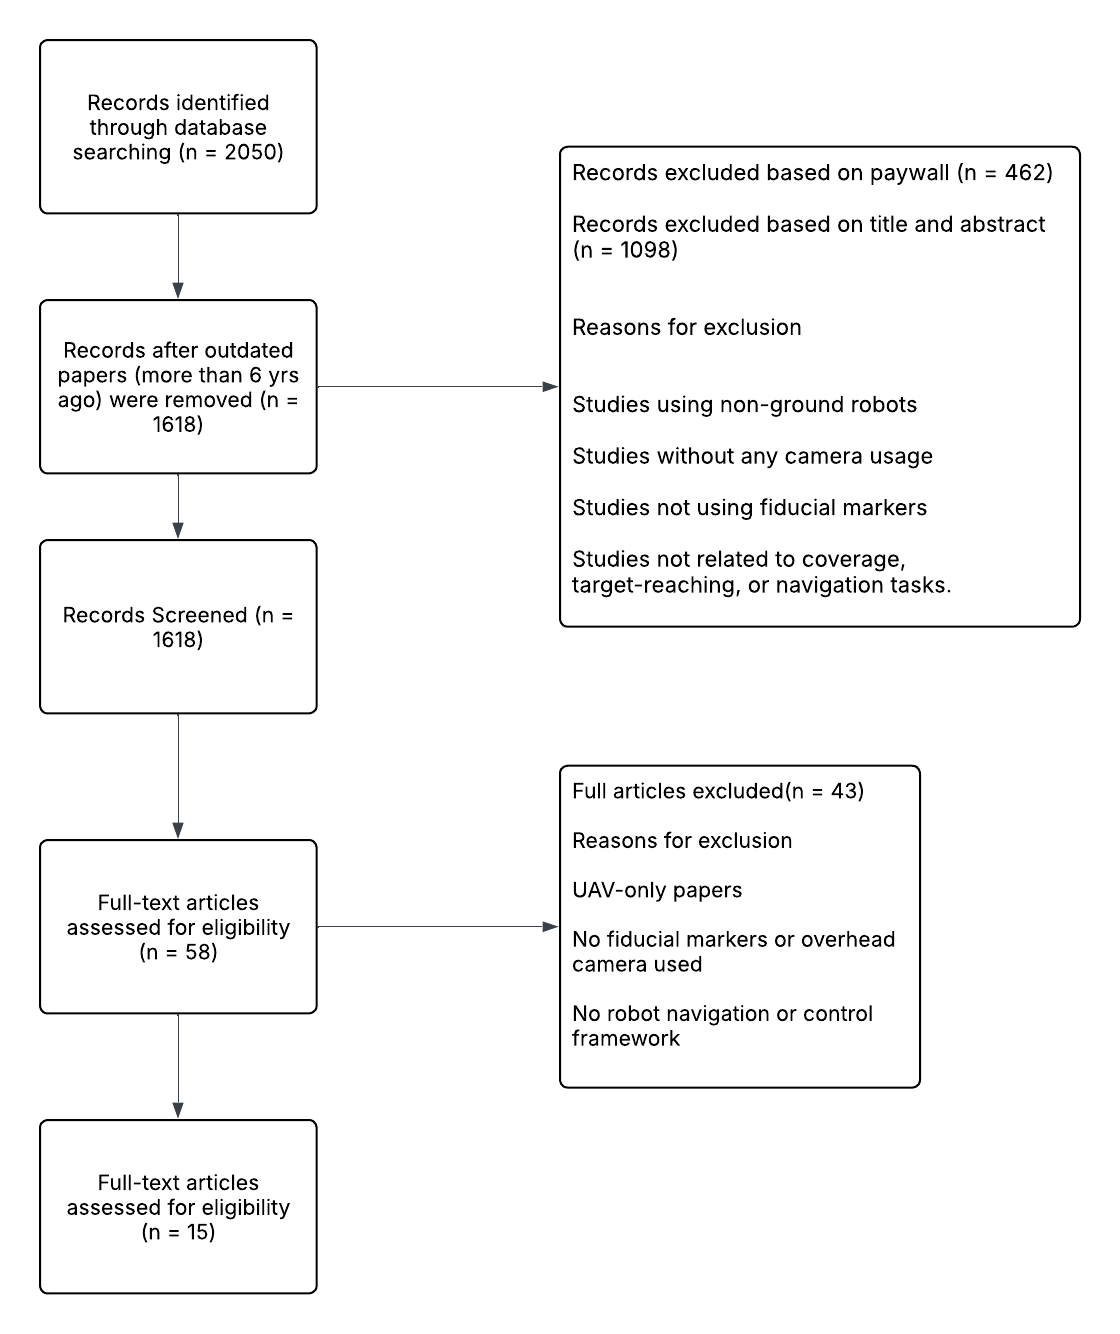
\includegraphics[width=0.7\linewidth]{chap2/images/figure_prisma.png}
    \caption{PRISMA 2020 Flowchart}
    \label{fig:figure_prisma}
\end{figure}

\section{Autonomous Navigation and Sensor Technologies}
Autonomous navigation fundamentally relies on a mobile robot’s ability to perceive its environment and determine its position relative to the environment. While autonomous navigation is a well established field, the hardware requirements for reliable performance remain a significant barrier for academic and low cost applications. In our review of literature on autonomous navigation, we found out that modern autonomous navigation relies on a heterogeneous sensor suite. Some of the most widely adopted technologies range from the classic RGB-D cameras , to innovations like event based sensors \citep{Gatesichapakorn2019ROSLidarRGBD, RodriguezMartinez2025VisionNavigationReview}. Recent multi-sensor approaches such as the work of \cite{Dai2023MultiSensorDocking}, who integrated LiDAR, YOLO-based AprilTag detection, and depth cues for autonomous docking, demonstrate how heterogeneous sensor fusion significantly improves docking precision and reliability in cluttered indoor environments. In this subchapter, we evaluate the advantages and disadvantages of each sensor technology.


\subsection{Monocular and Multicamera RGB Systems}
Monocular RGB cameras remain one of the most widely used sensing modalities in autonomous navigation due to their low cost, size, and ease of integration. Recent work demonstrates that deep learning greatly improves the capability of monocular systems, enabling better perception even without clear depth sensors. Research has shown that convolutional and transformer-based networks can infer scene geometry, obstacle layout, and traversability directly from RGB images 
\citep{Sleaman2022MonocularDNNNavigation}. Additional monocular systems, such as the neural-network-driven visual servoing framework by \cite{Jokic2019NNVisualServoing}, show how wide-FOV fisheye lenses combined with CNN-based controllers can enhance robustness even when depth cues are limited. Similarly, \cite{Ho2020PoseVisualServoing} demonstrated that pose-based visual servoing enhanced with lightweight deep-learning binarization improves tracking accuracy in resource-limited mobile robot platforms. These methods reduce hardware complexity while maintaining acceptable localization performance for indoor and structured environments.
Despite these advantages, monocular cameras suffer from an inherent depth ambiguity that can limit reliability in dynamic or cluttered spaces. Studies on monocular systems trained with deep reinforcement learning highlight that navigation performance largely depends on the variety of training environments \citep{Yokoyama2020DRLMonocularNavigation}. To help solve the depth limitation, recent research combines multiple deep learning modules and depth prediction to create better feature representations for navigation, as shown by \cite{Machkour2022MonocularNavigationMultipleDL}. These hybrid pipelines increase robustness but require more computational resources than classical monocular methods.

\subsection{RGB-D Cameras}
While Monocular and multi-camera RGB systems provide useful visual data for navigation, their lack of direct depth information restricts their robustness, especially in tasks requiring reliable 3D localization or obstacle avoidance. RGB-D cameras solve this problem by combining regular RGB images with depth information, producing a richer representation that simplifies tasks such as pose estimation, mapping, and collision detection. According to \cite{Civera2017RGBDOdometrySLAM}, RGB-D sensors are good alternatives to traditional range sensors like LiDAR because they are often cheap, compact, and require low-power, yet still provide both color and depth data that support 3D scene reconstruction. RGB-D sensing also appears in navigation pipelines such as the omnidirectional manufacturing-oriented robot proposed by \cite{Patruno2020VisionBasedOmniIndoor}, where combined RGB-D perception enables reliable autonomous movement in industrial indoor environments.

Many state-of-the-art approaches combine RGB-D data with odometry / SLAM pipelines to exploit this richer input. For instance, \cite{Gatesichapakorn2019ROSLidarRGBD} demonstrated a practical indoor navigation system using fused inputs from a 2D LiDAR and an RGB-D camera. This hybrid setup allowed a real mobile robot to navigate without a precomputed map. On the other hand, recent work such as \cite{Kostusiak2023EnhancingVOWithDepth} shows how modern deep-learning techniques can further improve performance: by refining noisy or incomplete depth maps (common with low-cost Kinect-like sensors), the study achieved more reliable indoor visual odometry under budget-friendly constraints.

\subsection{LiDAR and Camera-LiDAR Hybrids}
Recent studies highlight that combining LiDAR with cameras significantly improves autonomous navigation systems. According to \cite{Kolar2020DataFusionSurvey}, combining data from LiDAR and cameras lead to more accurate and robust mapping and localization, than just relying on either modality alone. There are studies that support this view, for example, \cite{DeSilva2018LidarWideAngleFusion}, designed a framework that  combined the use of LiDAR and wide-angle camera images and it resulted in significantly improved free-space detection performance. Hybrid LiDAR-vision architectures further align with the findings of \cite{Liu2022RobustLocalizationVisionCNN}, who showed that fusing CNN-based visual relocalization with progressive LiDAR scan-matching significantly enhances robustness under viewpoint changes and degraded visual conditions. However, these papers also highlight the limitation of the LiDAR-camera fusion which requires precise calibration and consistent environmental conditions that make real-time deployment more computationally demanding.

\subsection{Event-Based Cameras}
Event-based cameras output streams of “events” rather than fixed video frames, because of this, they offer compelling advantages for robotics and SLAM. According to \cite{Tenzin2024EventCamerasVSLAMSurvey}, event cameras deliver high temporal resolution, low latency, reduced power consumption and data bandwidth compared to traditional frame-based cameras. Additionally, the hardware architecture of this type of camera can efficiently handle the asynchronous event streams which enable low-power SLAM and perception on embedded robotic systems.

\subsection{Infrared and Thermal Imaging Sensors}
Infrared and thermal imaging sensors give strong advantages for autonomous robots especially in visually degraded and low-light environments. \cite{Papachristos_Mascarich_Alexis_2018b} showed that thermal imaging provides reliable localization for robots even in smoke, dust, or foggy conditions where performance of other cameras like RGB and LiDAR deteriorates. Similarly, recent work on Thermal SLAM by \cite{Salem2025ThermalSLAM}. demonstrates that temperature-based features can be used for object detection and tracking which improves localization regardless of lighting.

\subsection{Comparative Summary}
\begin{table}[H]
\centering
\setlength{\tabcolsep}{4pt} % reduce horizontal padding
\begin{tabular}{p{2.5cm} p{5cm} p{5cm}} % narrower columns
\hline
\textbf{Sensing Modality} & \textbf{Key Advantages} & \textbf{Major Limitations} \\
\hline
Monocular and Multicamera RGB &
\begin{itemize}
  \item Low cost, compact size, and ease of integration.
  \item Simplifies mapping and collision detection.
\end{itemize} &
\begin{itemize}
  \item Prone to noise or incomplete depth maps.
  \item Often limited to indoor ranges.
\end{itemize} \\
\hline
LiDAR \& Camera Hybrids &
\begin{itemize}
  \item Significantly improved free-space detection.
  \item More accurate and robust mapping than the single standalone of each part.
\end{itemize} &
\begin{itemize}
  \item Requires precise calibration.
  \item Computationally demanding for real-time deployment.
  \item Requires environmental consistency.
\end{itemize} \\
\hline
Event-Based Cameras &
\begin{itemize}
  \item High temporal resolution and low latency.
  \item Reduced power consumption and data bandwidth.
\end{itemize} &
\begin{itemize}
  \item Requires specific hardware architectures.
  \item Output is non-traditional (events) which requires specific processing.
\end{itemize} \\
\hline
Infrared \& Thermal Sensors &
\begin{itemize}
  \item Reliability in visually degraded conditions.
  \item Effective even in low-light, low visibility environments.
\end{itemize} &
\begin{itemize}
  \item Primarily focused on visually degraded conditions.
  \item Less feature rich for standard navigation.
\end{itemize} \\
\hline
\end{tabular}
\caption{Sensing modalities, advantages, and limitations.}
\label{tab:sensing_modalities}
\end{table}

As shown in Table 2.3, while LiDAR and Hybrid systems offer high accuracy, they suffer from high computational demands and calibration complexity. Conversely, Monocular RGB systems (Section 2.2.1) offer a balance of low cost and hardware simplicity. By leveraging Deep Learning—specifically the Neural Network architecture inherent in the DonkeyCar framework—this study aims to mitigate the 'depth ambiguity' limitation of monocular cameras by supplementing local vision with a global overhead supervisor (ArUco), thereby maintaining the low-resource benefits of RGB systems while improving navigation reliability.

\section{Computer Vision for Autonomous Robot Systems}
The computer vision systems in robotics systems serve as the eyes of the robot – providing vision that helps it recognize and understand its surroundings. Studies such as \cite{Alimovski2022VisionUrbanLocalization} also show that camera-only visual localization pipelines can remain effective even in complex, GPS-limited outdoor urban environments. Computer vision as defined by \cite{Vina2023CVInRoboticsIntegration}, is the technique where robotic systems use cameras and sensors to gather visual information.Then the information gathered is then processed by algorithms, which enable robots to perform complex tasks like assembly, quality control, and navigation. 

\subsection{LiDar and RTK-GPS and its Limitations}
LiDar and RTK-GPS (Real-Time Kinematic GPS), alone or in combination, are widely used to produce accurate mapping for vehicles \citep{DeMiguel2020ImprovedLidarProbabilistic, Thepsit2023LidarRTKGNSSINS}. However, there are several limitations that push for the implementation of alternative approaches for autonomous systems.

\subsubsection{Cost, Hardware, and Computational Requirements}
LiDar systems, as described by \cite{Whitaker2020GlobalLocalizationFiducialsIMU}, are often expensive and sizable for some applications. \cite{Lu2021LocalizationTechniquesReview} supports this idea in their study, concluding that LiDar is the most promising method for producing accurate, real-time localization among other approaches but suffers from the limitations of the system's computational ability, requiring more powerful CPU/GPU. This limitation poses a problem for smaller systems such as mobile robots where money, weight, and power consumption directly impact the navigation operations.

\subsubsection{GPS Signal Degradation and Denial}
RTK-GPS systems may suffer from extreme performance degradation or complete signal loss in a constrained environment such as urban canyons, underground or multi-level parking structures, tunnels, and indoor spaces \citep{Bhat2024MultiSourceGPSDenied, Fang2020MarkerValetParking, Jeon2021LaneAidedDeadReckoning}. Odometry errors accumulate fast without external correction, leading to inaccuracy in position estimates. \cite{Massa2020LidarGNSSDeniedRacing} resorted to alternative methods for a localization of self-driving racecars because GPS can be unreliable on racing tracks and in harsh environments. 

The limitations for LiDar and GPS collectively motivate the exploration of modern sensing modalities that can provide reliable localization in challenging scenarios where traditional systems struggle  \citep{Dreissig2023LiDARAdverseWeatherSurvey, Zhang2023AdverseWeatherPerceptionSurvey}. This  necessitates a need for developing alternative low‑cost computer‑vision approaches based on artificial fiducial markers that can provide reliable positioning without expensive sensors.

\subsection{Fiducial Marker Methods}
Fiducial markers are designed visual patterns which are machine or camera-detectable strategically placed within an environment to provide reliable localization mapping or pose estimation cues for autonomous systems. These visual markers serve as the landmarks that may offer multiple advantages over resource-intensive, natural or feature-based localization techniques. A broader mapping of marker-based navigation techniques is summarized in the systematic review by \cite{Alghamdi2025MobileRobotMarkersMapping}, which highlights the lightweight computational requirements, reliability, and adaptability of fiducial marker systems across diverse robotic domains.

In comparative studies of standard, custom, reflective, and infrared markers, fiducial markers generally offer high detection accuracy, robustness, and low computational cost, but their performance can still degrade under poor lighting conditions \cite{Alghamdi2025MobileRobotMarkersMapping}. Standard physical markers will include but not limited to, AR Tag \citep{Fiala2005ARTag}, AprilTag \citep{Olson2011AprilTag}, and AruCo markers \citep{GarridoJurado2014FiducialMarkers}.


\subsubsection{Operational Advantages}
When compared to localization methods like GPS RTK, the pragmatic advantages behind physical fiducial markers come from their ability to provide discrete, absolute position fixes that can correct accumulated drift in dead-reckoning systems \citep{Park2023FusionLocalizationAirplane, Xu2023VisualNavigationUAV}

Markers also facilitate the creation of persistent maps with known landmark positions. Unlike natural feature-based SLAM, which must continuously track and update potentially ambiguous environmental features, marker-based systems can rely on the stable, unambiguous identity and position of installed markers. This stability simplifies map maintenance and enables more predictable localization performance \citep{MunozSalinas2018SPMSLAM, Pfrommer2019TagSLAM, Wang_Zhang_Zhu_Hu_Deng_He_Kang_2023}. 

\subsubsection{Applications in Autonomous Systems}
Fiducial markers were leveraged to localization for vehicle parking in a GPS-denied setting like an underground parking lot for precise autonomous driving \citep{Fang2020MarkerValetParking}. Moreover, indoor autonomous drones use ceiling or wall mounted markers for positioning during warehouse inventory and structural examination tasks \citep{Nahangi2018UAVFiducialConstruction}. Marker systems have also been applied in assistive indoor navigation, such as the ARUCO-based pan-tilt camera system demonstrated by \cite{Adapa2019AutonomousMapping} for improving mobility support for blind and visually impaired users. Overhead or airborne localization frameworks similarly leverage markers, as seen in \cite{Xu2023VisualNavigationUAV}, who demonstrated a UAV-based visual navigation method using squared planar fiducials for orientation and path-following.

These applications share a common theme: they operate in environments where GPS is unavailable or unreliable, infrastructure modification is feasible, and cost-effective localization solutions are essential. Fiducial markers address these themes by providing a pragmatic middle ground between expensive LiDAR systems and drift-prone dead-reckoning approaches. The following section (2.5.3) details how these fiducial marker principles are realized in marker-based localization and mapping architectures, with a focus on ArUco-based systems.

\subsection{Marker-Based Localization, Mapping, and ArUco Systems}
Building on the general properties of fiducial markers outlined in Section 2.2.2, this section examines marker-based localization and mapping pipelines, emphasizing ArUco-based implementations in autonomous vehicles and robots.

\subsubsection{Detection and Pose Estimation}
Planar fiducial marker systems usually follow a structured pipeline that begins with image acquisition and proceeds through marker detection, corner localization, and pose estimation. In common implementations such as ArUco, candidate markers are extracted by thresholding and contour detection, followed by decoding of the internal binary pattern to recover marker identity and reject false positives \citep{Rosebrock2024ArucoPyImageSearch}. Once the four marker corners are localized in image coordinates and associated with a known marker size, the perspective‑n‑point (PnP) algorithm is used together with the camera calibration parameters to obtain the 6‑degrees-of-freedom (6-DoF) transformation between the marker frame and the camera frame \citep{Braun2022RobotAtFactoryLocalization, Fang2020MarkerValetParking}. This geometric formulation avoids any need for training data, and it provides an interpretable pose estimate that can be directly integrated into downstream localization and mapping pipelines.

\subsubsection{Robot and Camera Pose Tracking with ArUco}
Real-time implementations such as the UAV-mounted camera system in \cite{Waqas2022FiducialUAVSHM} confirm that marker-based pose tracking remains feasible even under dynamic motion, non-static camera poses, and rapid changes in scene geometry. Additionally, lightweight educational platforms, such as those in the Duckietown initiative by \cite{Krinkin2019DuckietownCalibration}, highlight how careful camera calibration and wheel-encoder integration support accurate pose estimation even on low-cost robotic systems.
When fiducial markers are deployed in the environment, each ArUco detection yields a relative pose measurement between the camera and the corresponding marker. Assuming a calibrated camera and known marker dimensions, these measurements can be expressed in metric units and transformed into a robot-centric or world-centric frame, enabling continuous tracking of the robot’s position and orientation as it moves through the environment \citep{Montecchio2022FiducialsUAV, Zhou2022UAVIndoorLocalization}. In practice, the system accumulates a time series of marker-based pose updates, which are combined with kinematic information such as wheel odometry to produce a smooth estimate of the robot trajectory in GPS‑denied settings.



\subsubsection{ArUco-based Planar Task-Space Localization}
Aside from providing global or relative pose measurements, planar fiducial configurations can be used to define local task spaces through homography estimation \citep{Braun2022RobotAtFactoryLocalization}. Numerous experimental systems have demonstrated the practicality of ArUco markers for autonomous vehicle and robot localization.

By placing multiple ArUco markers at the corners of a region of interest, \cite{Huang2022OptimizingMarkerPlacement} explored an optimized system that can compute a projective transformation between image coordinates and a planar world coordinate frame aligned with the physical surface. In addition, \cite{Rosner2025MultimodalIndoorDroneDataset} follows this idea for indoor drone tracking through markers on walls that define a room coordinate system (inside-out tracking). This demonstrates the efficacy of fiducial markers to provide planar task-space localization. \cite{Oh2025RegressionDockingAruco} applied this system for docking stations to achieve robust positioning with low-cost cameras and embedded processors. 

\subsubsection{Sensor Fusion Architectures}
In conventional autonomous systems, marker-based pose estimates are typically fused with proprioceptive sensors to compensate for intermittent visibility and measurement noise \citep{Kumar2023LocalizationSurveyAV}. Extended Kalman filters, error-state Kalman filters, and particle filters are widely used to combine discrete, absolute pose fixes from fiducial markers with continuous estimates derived from wheel encoders and inertial measurement units \citep{DeLaPuente2025VisionRangeAMCL, Ullah2020FilterLocalizationEvaluation}. Marker–odometry fusion has also been demonstrated effectively by \cite{Alam2023FiducialPFLocalization}, who showed that integrating AprilTag observations with particle filtering reduces drift and improves localization accuracy in indoor autonomous robots. In systems like these, the prediction step propagates the robot state forward using odometry or motion models, while the update step incorporates new marker observations when available, bounding drift and improving robustness when there is sensor noise and environmental disturbance.

\subsubsection{Marker-aided SLAM and Mapping}
In recent meta, mapping for autonomous robots are commonly carried out through LiDAR vision, which is costly and complex when it comes to maintenance \cite{Chen2025MapsAutonomousDrivingSurvey}. Traditional Marker-aided SLAM formulations incorporate fiducial markers as explicit landmarks in the map, rather than relying solely on natural point or line features \cite{Tourani2023MarkerBasedVisualSLAM}. In graph-based SLAM, markers are represented as nodes with fixed or estimated poses, and edges encode relative constraints between robot poses and marker observations; optimization of this graph improves both robot trajectories and marker maps \cite{MunozSalinas2018SPMSLAM}. This approach simplifies data association, because each marker carries a unique identifier, and supports persistent, globally consistent maps that can be reused across sessions, which is particularly advantageous in structured environments such as parking facilities and industrial halls.

Recent implementations reinforce the practical value of this paradigm. For example, \cite{Tolenov2024SelfLocalizationMapping} demonstrated a real-time camera-based SLAM pipeline capable of mapping unknown indoor environments without the use of LiDAR, showing that lightweight vision systems can be competitive when supported by robust tracking and optimization. Marker-enhanced localization pipelines also appear in aerial–ground hybrid systems such as \cite{Asif2020TetheredDroneLocalization}, where a tethered UAV and ground robot perform collaborative localization using deep neural networks supplemented by intermittent fiducial marker detections. These studies highlight how marker-aided SLAM can reduce cost, simplify data association through unique IDs, and enable persistent, reusable maps which are particularly beneficial in structured indoor environments.

\subsubsection{Gap Analysis for Marker-Based Detection and Localization}
While the literature establishes that marker-based sensor fusion and SLAM architectures (discussed in Sections 2.5.3.4 and 2.5.3.5) provide robust state estimation, they inherently introduce significant computational complexity and latency due to the iterative nature of Kalman filtering and graph optimization. Moreover, these traditional pipelines rely heavily on explicit state estimation. This requires the system to calculate the exact coordinates at every time step before making control decisions. This dependency introduces architectural complexity and computational overhead. Section 2.6 reviews recent advancements in deep learning for robot control, providing further justification for the shift away from traditional pose estimation toward end-to-end architectures.

\subsection{Modern Detection and Real-Time Systems}
Autonomous robots require vision-based localization pipelines that operate under strict real-time and resource constraints, often on embedded platforms such as single-board computers or low-power system-on-chip devices. The detection and pose estimation of fiducial markers must run at sufficient frame rates to support closed-loop control, while sharing computational resources with other perception and control modules. This has motivated a line of work focused on optimizing fiducial detection algorithms, memory usage, and numerical routines so that marker-based localization remains feasible on platforms with limited CPU, GPU, and power budgets \cite{Yulianto2025LightweightArucoDetection}.

\section{Deep Learning Approaches for Robot Control Strategies}
The integration of neural networks in autonomous systems have shifted the industry standard from hand-coded features, to data driven methodologies. In the context of autonomous mobile robot navigation, deep learning techniques have been increasingly used to process complex sensory data and generate navigational decisions. Upon reviewing literature, a survey from \cite{Xiao2022MLMotionPlanningSurvey} shows three deep learning paradigms for robot navigation; End-to-End Learning (E2E), Learning Subsystems, and Learning Components. Additionally, specific neural network architectures and training methodologies, referred to here as deep learning techniques, are employed across these paradigms to handle varied input modalities and control objectives. Recent marker- and vision-based navigation studies reinforce this trend. For instance, \cite{Liu2022RobustLocalizationVisionCNN} demonstrated that CNN-based relocalization can significantly improve pose recovery within a hybrid LiDAR-vision localization framework, showing how learned perception compensates for degraded geometric features. Deep neural controllers have also been applied to monocular systems, such as the visual servoing approach by \cite{Jokic2019NNVisualServoing}, which uses fisheye camera imagery to control a wheeled mobile robot. Similarly, \cite{Ho2020PoseVisualServoing} leveraged lightweight deep-learning binarization to enhance pose-based visual servoing for resource-constrained mobile robots. Hybrid aerial-ground systems such as \cite{Asif2020TetheredDroneLocalization} also illustrate how DNNs can infer relative positions between robots when fiducial marker signals are intermittent or partially occluded.
Together, these systems demonstrate that deep learning serves not only as a replacement for classical control but also as a complementary module for perception, relocalization, and decision-making within modern autonomous navigation architectures.

\subsection{Deep Learning Scopes}
The application of deep learning in autonomous mobile robot navigation is categorized by how much of the classical navigation stack (perception, localization, planning, and control) is replaced by neural networks. If the whole system is replaced with a neural network (E2E), if only subsystems of the navigation system are replaced (Learning Subsystems), or if only components (Learning Components).

End-to-End (E2E) Learning seeks to replace the classical navigation stack with a single deep neural network that maps raw inputs directly to control actions. This approach centralizes the process by integrating it into a single neural network process. \cite{Kim2018EndToEndNavigation}  demonstrated this by developing a deep learning model that processes RGB camera data to output steering in a single step. Similarly, \cite{Pierre2018EndToEndFollowing} applied E2E learning to robotic following behaviors, proving that a single network could learn complex tracking tasks without explicit object recognition modules.

Deep Learning Components, unlike E2E, involve replacing a single processing step within a module with a deep learning model. The most common application is in the perception module, where Convolutional Neural Networks (CNNs) replace manual feature extractors to perform object detection or semantic segmentation. For example, \cite{Redmon2016YOLO} introduced YOLO, a real-time object detection system that serves as a perception component, feeding bounding box coordinates to a classical costmap or planner. In this scope, the neural network does not make navigational decisions; it strictly provides structured information to a classical algorithm.

Deep Learning Subsystems replace an entire subprocess in the multi-step process of the autonomous robot navigation stack, while retaining the classical methods for the other parts. One such example is \cite{Mohanty2016DeepVO} DeepVO architecture proposal. The deep learning architecture replaces the classical visual odometry system with a Recurrent Convolutional Neural Network (RCNN). This subsystem takes raw video as input and outputs the robot's pose, directly replacing the localization module while leaving the planning and control modules untouched. A similar study from \cite{Faust_Ramirez_Fiser_Oslund_Francis_Davidson_Tapia_2017} proposed "PRM-RL," which replaces the local path planner subsystem with a Reinforcement Learning agent to handle dynamic obstacle avoidance, while still relying on a classical Probabilistic Roadmap (PRM) for global path planning. 

\subsection{Deep Learning Techniques}
Navigation systems often rely on specific neural network architectures and learning algorithms to process distinct data inputs, and generate control policies as outputs. Upon critical review on Literature, it is evident that the deep learning approaches of autonomous mobile robot navigation are driven by three architectural paradigms: Convolutional Neural Networks (CNNs), Recurrent Neural Networks (RNNs), and Vision Transformers (ViTs).

Convolutional Neural Networks are the most widely used approach in these systems. This can be attributed to the fact that CNNs are the best fit for the navigation pipeline. CNNs are best suited for processing spatial data such as camera images, depth maps, and lidar projections. The CNN can extract localized information from edges and textures to semantic level concepts, allowing robots to interpret complex environments reliably and efficiently \citep{LeCun2015DeepLearningNature}. This makes CNNs the best fit for perception tasks such as obstacle detection \citep{Eigen2014DepthSingleImage, Ronneberger2015UNet, Redmon2016YOLO}. This makes it the best fit for replacing the classical localization part of the navigation stack.

Recurrent neural networks (RNNs) are widely used in robot navigation due to their ability to model dependencies in sequential data such as robot odometry, velocity history, etc. Unlike CNNs, RNNs with LSTMs, and or GRUs are essential for predicting sequential robot trajectories, estimating future states, and generating smooth control commands \citep{Hochreiter1997LSTM, Cho2014RNNEncoderDecoder}. Recent Research incorporates RNNs with reinforcement learning or hybrid deep learning pipelines to better model robot-to-environment interactions. One example is the hybrid RNN architecture proposed by \cite{Radha2025HybridRNNNavigation} which demonstrates an improvement on optimization of path planning and collision avoidance by fusing temporal motion cues with spatial features extracted from CNNs Although studies also show that that RNN-based models significantly improve localization accuracy by including historical context, reducing hallucinations and localization drift, denoising movements, specifically in environments where GPS is not available \citep{Ichter2018LearningSamplingDistributions, Weng2019MotionForecastingRNN}.

Vision Transformers (ViTs) are a newer deep learning technique that is used in robot navigation, leveraging the breakthroughs in self-attention and the transformer model for vision based tasks. Unlike CNNs, which look at a group of fields at a time, CNNs process the data, its dependencies, and the semantics of each datapoint relative to each other. This helps robots interpret the whole environment, and consequently, plan out safe paths more effectively. \citep{Dosovitskiy2021ViT, Khan2022TransformersVisionSurvey}. Recent studies show that ViTs outperform CNNs in tasks requiring higher level semantic understanding or contextual awareness, such as large scale mapping, multiple map localization, contextual path planning, etc. \citep{Chen2021TransTrack}. Their ability to maintain performance under viewpoint changes, lighting variations, and occlusion makes them increasingly relevant for robust real-world navigation.

\section{Theoretical Framework}
This section outlines the mathematical models and fundamental theories utilized in the development of the autonomous navigation system. Specifically, it discusses the geometric principles of homography for localization, the algorithmic basis of fiducial marker detection, and the architecture of the deep learning approach used in the study.
\subsection{Projective Geometry and Planar Homography}
Since this study uses a single overhead camera to track a robot on a flat floor, the relationship between the camera’s image plane and the real world ground plane is defined by a planar homography. In computer vision, homography is defined as a fundamental projective transformation that maps points from one planar surface to another \cite{Hartley2003MultipleViewGeometry}. In our case, given an image point $p = (u, v, 1)^{t}$ and a corresponding point in the ground-plane coordinate system $p' = (x, y, 1)^{t}$, the planar homography relates them as 

\[
s
\begin{bmatrix}
x \\[2pt]
y \\[2pt]
1
\end{bmatrix}
=
H
\begin{bmatrix}
u \\[2pt]
v \\[2pt]
1
\end{bmatrix}
=
\begin{bmatrix}
h_{11} & h_{12} & h_{13} \\
h_{21} & h_{22} & h_{23} \\
h_{31} & h_{32} & h_{33}
\end{bmatrix}
\begin{bmatrix}
u \\[2pt]
v \\[2pt]
1
\end{bmatrix}
\]

where 
\begin{itemize}
    \item $s$ is an arbitrary scaling factor,
    \item $H$ is the $3\times3$ homography matrix,
    \item $(u,v)$ are the pixel coordinates of the marker,
    \item and $(x,y)$ are the metric coordinates on the floor.
\end{itemize}



To solve for the matrix $H$, at least four point correspondences are required. This study leverages the Direct Linear Transformation (DLT) algorithm to compute $H$ using calibrated anchors at the corners of the navigation arena, allowing for the real-time conversion of visual data into metric position estimates \citep{Szeliski2010ComputerVisionBook}.

\subsection{Neural Networks and Convolutional Neural Networks (CNNs)}
The control strategy that we proposed in this study is a CNN-based perception to actuation framework to provide end-to-end navigation controls. Unlike classical control methods like PID, which rely on a mathematical method for error correction, this study uses neural networks to approximate the non-linear relationship between the visual input and motor control, effectively emulating the thought process of a human driver. A neural network is a model that aims to imitate the functions of a human brain. It is made up of interconnected nodes (neurons) that are organized into different layers \citep{Goodfellow2016DeepLearning}. The fundamental operation involves transforming input data x into an input y through a series of weighted sums and non-linear activation functions:

\[
h_i = f_i\!\left(W_i h_{i-1} + b_i\right)
\]
where $h_i$ is the output of the $i$-th layer, $W_i$ and $b_i$
are the weight matrix and bias vector, and $f_i$ is the nonlinear
activation function.


This study employs a Convolutional Neural Network (CNN) architecture, which is highly effective for processing grid-like data such as images \citep{LeCun2015DeepLearningNature}. CNNs are characterized by three primary layer types that allow the system to learn spatial hierarchies automatically.

Convolutional Layers. These layers apply a set of kernels that slide over the input image, performing convolution operations to extract spatial features such as edges, textures, etc. The operation is defined as:
\[
(K * I)(i,j) =
\sum_{m}\sum_{n}
I(i - m,\, j - n)\, K(m,n)
\]

where $I$ is the input image, $K$ is the kernel, and $(i,j)$ are the
spatial coordinates.



Pooling Layers. These layers downsample the feature maps, reducing the dimensionality and the number of parameters. This helps make the features robust to slight shifts or distortions (e.g., Max-Pooling) while lowering the computational load.

Fully Connected Layers. Typically placed at the end of the CNN, these layers flatten the high-level features extracted by the convolutional and pooling layers and map them to the final output. In this study, the output corresponds to the continuous motor power commands (ie. left and right wheel velocities for Ackermann steering).

In the context of this research, CNN functions as an end-to-end policy network. It takes the homography-transformed overhead image, augmented with a digitally rendered coverage path, as input and regresses the optimal motor controls required to track that path. The network is trained using Behavioral Cloning, where the loss function (e.g., Mean Squared Error) minimizes the difference between the network's predicted actions and the human demonstrator's commands during the data collection phase. This approach allows the system to learn complex path-following behaviors directly from visual data, serving as a learned path follower component that bridges the gap between perception and control.

\subsection{Imitation Learning and Behavioral Cloning}
The study uses Imitation Learning as its deep learning approach. Imitation learning is the industry standard end-to-end approach based on our literature on Chapter 2. Imitation learning assumes access to expert demonstration. The goal is to learn a control policy  that mimics the behavior of the expert given specific state observations \citep{Osa2018ImitationLearningSurvey}.
More specifically, this study implements Behavioral Cloning, the simplest and most direct form of Imitation learning. Using this, the problem of learning a robot’s control policy is then reduced to a supervised learning task. The system collects a dataset $D$ consisting of $N$ pairs of observations and expert actions:
\[
D = \{(s_i, a_i)\}_{i=1}^{N}
\]
where $s_i$ represents the state observation (input) at time step $i$,
and $a_i$ represents the expert action (output) at time step $i$.




    \chapter{Methodology}

\section{System Overview \& Architecture}
The proposed system implements a centralized, vision-based autonomous navigation architecture inspired by end-to-end learning paradigms. Unlike traditional autonomous robots that rely on onboard sensors (e.g., LIDAR, onboard cameras) and local processing, this framework offloads the computational workload to a remote workstation, utilizing a Bird’s Eye-view or overhead perspective. The architectural data flow, detailing the transition from physical sensing to robot actuation, is illustrated in Figure 3.1.

\begin{figure}[!ht]
    \centering
    {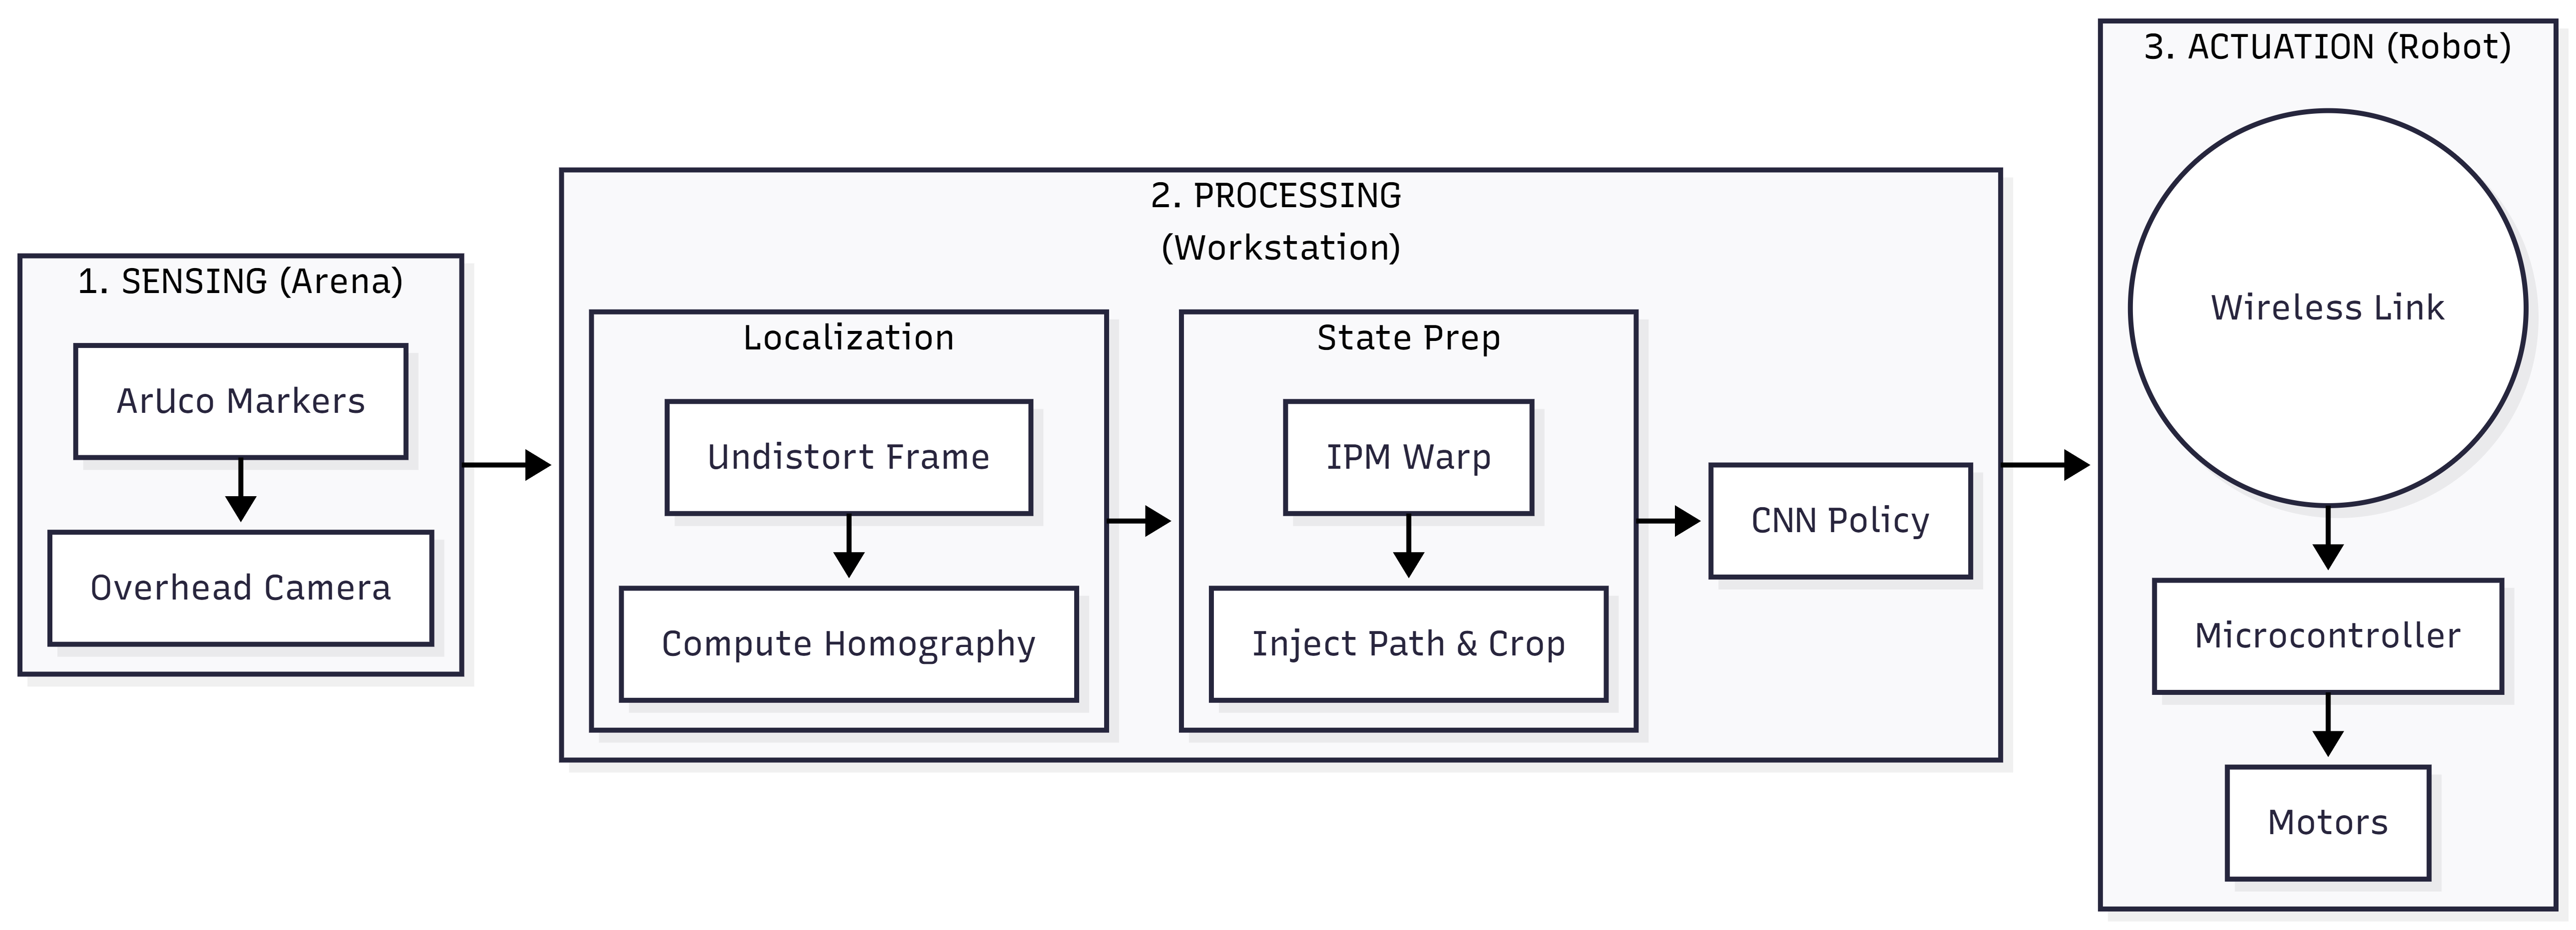
\includegraphics[width=1.0\textwidth]{images/figure3_1.png}}\qquad
    \caption[Short Caption]{System Architecture.}        
    \label{fig:3.1}
\end{figure}


As depicted in Figure~\ref{fig:3.1}, the system architecture is divided into three functional subsystems: sensing, processing, and actuation. Together, these components form a closed-loop control pipeline for autonomous navigation.

\begin{itemize}
    \item \textbf{Sensing Subsystem (Arena):}  
    Located in the physical environment, this block consists of an overhead camera and fixed ArUco markers. The camera captures the entire operational arena and provides the raw visual input used by the system. The ArUco markers act as reference points for geometric correction and spatial alignment.

    \item \textbf{Processing Subsystem (Workstation):}  
    This block contains the core intelligence of the system and executes a two-stage processing pipeline:
    \begin{itemize}
        \item \textbf{Localization and State Preparation:}  
        The system detects ArUco markers to compute a homography matrix, which warps the angled camera feed into a standardized top-down bird’s-eye view using inverse perspective mapping (IPM). The transformed image is cropped and augmented with the target navigation path to form the system state.
        
        \item \textbf{CNN-Based Policy Inference:}  
        The pre-processed visual state is fed directly into a convolutional neural network (CNN), which serves as an end-to-end behavioral policy mapping visual observations directly to low-level motor control commands.
    \end{itemize}

    \item \textbf{Actuation Subsystem (Robot):}  
    The inferred control commands, including steering and throttle signals, are transmitted wirelessly via Wi-Fi or Bluetooth to the mobile robot. The robot’s onboard microcontroller receives these commands and drives the motors, completing the closed-loop control cycle.
\end{itemize}

\section{Hardware Setup}

\subsection{Robot Platform}
The mobile agent utilized in this study is a custom-built differential drive robot designed for low-latency execution of remote commands. The platform is intentionally minimized to function as a "remote-controlled" agent, removing the need for heavy onboard computation.

    \begin{itemize}
        \item \textbf{Chassis and Drivetrain:} 
        The robot is built on a standard 2-wheel drive (2WD) chassis with a caster wheel for stability. It utilizes two DC gear motors configured for Differential Drive kinematics, allowing for zero-radius turning and precise heading adjustments.
        \item \textbf{Microcontroller:}
         The robot is equipped with a low-cost microcontroller (e.g., Raspberry Pi 4 or Nvidia Jetson Nano) acting as a communication bridge. Its sole function is to receive data packets from the central workstation and convert them into Pulse Width Modulation (PWM) signals.
         \item \textbf{Motor Driver:}
          An H-Bridge motor driver (e.g., L298N or TB6612FNG) is used to interface the microcontroller with the DC motors, providing the necessary current amplification and direction control.
          \item \textbf{Power Supply:}
           The system is powered by a Lithium-Ion battery pack (e.g., 2S or 3S 18650 configuration), regulated to provide stable voltage to the microcontroller and raw power to the motor driver.
    \end{itemize}

\subsection{Environment Setup}
The experimental environment is a controlled, structured arena designed to implement computer vision processing. A single high-definition RGB webcam (Logitech BRIO) is mounted at a fixed height above the area. The camera is positioned at an angle to cover the entire operational area. While the camera is angled, the software pipeline corrects this perspective distortion mathematically. The arena consists of a flat, non-reflective surface (to minimize glare and specular highlights that could confuse the CNN). The boundaries of the Region of Interest (ROI) are physically defined by four ArUco markers fixed at the corners. These markers serve as the static reference anchors for the system's homography calibration. All image processing, neural network training, and real-time inference are performed on a dedicated laptop or desktop computer equipped with a GPU. This workstation runs the Python-based control software, processes the camera feed via USB, and broadcasts control commands to the robot over the local wireless network.




\section{Camera and System Calibration}
To ensure that the visual input fed into the neural network accurately represents the physical world, the system undergoes a rigorous calibration process. This separates the intrinsic properties of the camera (lens distortion) from the geometric relationship between the camera and the arena (homography).
The goal of intrinsic calibration is to estimate the camera matrix K (focal lengths and principal point) and distortion coefficients so that the image pixels and rays can be mapped in 3-D. Firstly, we introduce the pinhole model \citep{Hartley2004}, where a scene view is formed by projecting 3D points into the image plane using a perspective transformation. 

\begin{equation}
    s \begin{bmatrix} u \\ v \\ 1 \end{bmatrix} = K \begin{bmatrix} X \\ Y \\ Z \\ 1 \end{bmatrix}
\end{equation}

\noindent where:
\begin{itemize}
    \item $(X, Y, Z)$ are the coordinates of a 3D point in the world coordinate space.
    \item $(u, v)$ are the coordinates of the projection point in pixels.
    \item $s$ is a scaling factor.
\end{itemize}

However, camera lenses introduce lens distortion where lines may appear deformed. Mostly, these distortions are classified as radial distortion and slight tangential distortion (Brown, 1966). Webcam cameras, particularly the wide-angle lens on the Logitech BRIO used in this study—introduce radial and tangential distortion. To address this, the pinhole model above is augmented with a vector of distortion coefficients. These distortions are addressed using the following distortion model:

\noindent Radial Distortion:
\begin{equation}
    x_{corrected} = x(1 +k_1r^2 + k_2r^4 + k_3r^6)
    \label{radialDistortX}
\end{equation}
\begin{equation}
    y_{corrected} = y(1 +k_1r^2 + k_2r^4 + k_3r^6)
    \label{radialDistortY}
\end{equation}

\noindent Tangential Distortion
\begin{equation}
    x_{corrected} = x + [2p_1xy + p_2(r^2 + 2x^2]
\end{equation}
\begin{equation}
    y_{corrected} = y + [p_1(r^2 + 2y^2) + 2p_2xy]
\end{equation}

\noindent where:
\begin{itemize}
    \item \(k_1, k_2, k_3\) are radial coefficients,
    \item \(p_1, p_2\) are tangential coefficients and
    \item \(r^2 = x^2 + y^2\)
\end{itemize}

In OpenCV \citep{Bradski2000OpenCV}, these are grouped into a distortion vector that typically contains radial terms and tangential terms. All distortion coefficients are treated as intrinsic parameters of the camera. And once these coefficients are estimated, they remain valid for that camera regardless of the scene and can be reused at varying image resolutions, with only the focal length and principal point scaled if the resolution changes. 

\noindent\textbf{Calibration Procedure}

Intrinsic parameters are obtained using a standard checkerboard calibration method based on \cite{Zhang2000CameraCalibration}. We use the function \verb |calibrateCamera| then a planar checkerboard with known square dimensions is captured from multiple viewpoints. The inner corners are detected in each image, creating a set of 2D pixel observations corresponding to known 3D grid coordinates. The function uses the Levenberg-Marquardt optimization algorithm \citep{Levenberg1944LeastSquares} to minimize the reprojection error, defined as the sum of squared distances between the observed feature points (detected corners) and the projected object points (computed using current estimates of K and distortion coefficients). This process outputs the optimal intrinsic matrix and distortion vector, which are then stored for real-time image correction.

\section{Perception and Localization Module}
To enable autonomous navigation, the system requires a robust method to define the valid operational area and pre-process visual data for the neural network. This is achieved using fiducial markers to define the Region of Interest (ROI) and applying a projective transformation to normalize the visual input. This perception module operates in two distinct phases:

\begin{itemize}
    \item Initialization Phase: A one-time setup process that detects static arena boundaries and computes the coordinate mapping (from Section 3.3.2).
    \item Runtime Phase: A continuous loop that corrects and warps visual data in real-time for the control policy.
\end{itemize}

\subsection{ArUco Marker Detection}
\label{sec:3.4.1}
The localization pipeline begins with the detection of ArUco markers (Garrido-Jurado et al., 2014),  to define the Area of Interest (AOI). We utilize the \verb|DICT_4X4_50 |dictionary (4x4 bit grid, 50 unique IDs), which offers a balance between decoding speed and false-positive rejection.

\noindent\textbf{Marker Configuration and Corner Assignment}

To resolve the ambiguity of the arena’s orientation and prevent the coordinate system from mirroring or rotating if the camera placement changes, specific unique IDs are assigned to the four physical corners of the operational area. This fixed assignment acts as a ground truth for the homography estimation. The configuration is explicitly defined as follows:
\begin{enumerate}
    \item Top-Left (TL): Marker ID 0
    \item Top-Right (TR): Marker ID 1
    \item Bottom-Right (BR): Marker ID 2
    \item Bottom-Left (BL): Marker ID 3
\end{enumerate}

During the initialization part, the system does not simply accept any four detected markers. It filters the detected markers to find these specific IDs. Once these markers are found, they are sorted into a strictly ordered list \verb|[TL, TR, BR, BL]|, which is then used to get the homography matrix discussed in the later section.

Essentially, detection is performed on the undistorted frame. If detection were performed on the raw frame, the resulting Homography matrix would incorporate lens distortion, leading to a warped coordinate system where straight trajectories appear curved. By undistorting first, we ensure that the detected marker corners correspond to linear projective geometry.

\noindent The detection pipeline proceeds as follows:
\begin{enumerate}
    \item Preprocessing: The input RGB frame is converted to grayscale to simplify intensity analysis.
    \item Candidate Extraction: Adaptive thresholding is applied to segment black borders. Contours are extracted from the thresholded image and filtered based on convexity and square geometry.
    \item Bit Extraction and Decoding: The inner region of candidate squares is divided into a grid. The pixel intensity of each cell is analyzed to form a binary matrix.
    \item Corner Refinement: To ensure high-precision localization, corner positions are refined to sub-pixel accuracy using the \verb|cornerSubPix| algorithm
\end{enumerate}

The output is a set of four ordered corner coordinates from the undistorted image. It should be noted that these markers are not attached to the robot, they serve only to anchor the global coordinate system of the arena for the homography calculation.

\subsection{Planar Homography Estimation}
\label{sec:3.4.2}
Unlike the usual 3D pose estimation, this study limits the robot’s movement to a 2D planar surface. Additionally, the geometric relationship between the camera’s image plane and the physical world plane is modeled as a Planar Homography \citep{Hartley2003MultipleViewGeometry}. A homography is an invertible projective transformation that maps points from one plane (image pixel plane) \(p = [u,v,1]^T\) and a world coordinate \(P_w = [x,y,1]^T\) is given by:

\begin{equation}
    s[u,v,1] = H [u,v,1]
\end{equation}

where \(H\) is a \(3 \times 3\) matrix with 8 degrees of freedom

To compute H, we utilize the set of four physical points obtained from the ArUco markers (Section \ref{sec:3.4.1}), placed at the corners of the area of interest. Theoretically, this is solved using the Direct Linear Transformation (DLT) algorithm \citep{AbdelAziz2015DLT}. This algorithm rewrites the correspondence equation \(sx' = Hx\)  into a system of linear equations of the form \(Ah = 0\), where \(h\) is a vector containing the entries of \(H\). 

Since exactly four corresponding point pairs are established using the sorted ArUco IDs, we utilize the \verb|getPerspectiveTransform| function in OpenCV. This function computes the \(3 \times 3\) transformation matrix analytically. This method relies on the ground-truth correspondence provided by the unique marker IDs, which establishes a deterministic and geometrically accurate mapping.

\noindent \textbf{Perspective Warping (Runtime Application)
}

During runtime, the raw camera feed, which contains the arena viewed from an angle as well as irrelevant background noise is transformed using Perspective Warp. Leveraging the pre-computed \(H\), we map the entire input frame to a standardized top-down view. This is done through the use of the \verb|warpPerspective| function from OpenCV.

\begin{equation}
    Img_{world} = warpPerspective(Img_{raw}, H)
\end{equation}

This transformation creates a rectified "Bird's Eye View" image where the four corner markers perfectly align with the corners of the image frame. This ensures that the Convolutional Neural Network (CNN) receives an input that is geometrically constant regardless of slight shifts in camera placement or angle. This warped image serves as the direct input to the End-to-End control network, allowing the model to infer the robot's position and orientation from the visual features of the robot relative to the arena floor.

\subsection{Grid Map and Obstacle Representation}

To enable path planning and state observation, the continuous world coordinates are discretized into a Grid Map (Occupancy Grid). To define the grid, the area of interest is divided into \(N \times M\) matrix of cells, where each cell represents a fixed physical area defined by the resolution \(\delta\) (meters per cell). The mapping from World Coordinates \((x, y)\) to Grid Indices \((r, c)\) is defined as:

\begin{equation}
    c = |\frac{{x-x_{min}}}{\delta}|, r = |\frac{y-y_{min}}{\delta}|
\end{equation}

\noindent where:
\begin{itemize}
    \item \((x, y)\) are the metric coordinates of the point on the arena floor.
    \item \((x_{min}, y_{min})\) is the origin of the area in world coordinates.
    \item \(\delta\) is the resolution. 
\end{itemize}

We designated cells inside the area of interest between two states, free and obstacle. A cell in the grid matrix \(\bold{B}\) is assigned a binary value, a cell \(G[r,c]\) will be set to zero to denote an empty or clear space, which is safe for robot traversal. On the other hand, a cell will be set to one to denote an obstacle or restricted area.

This binary grid serves as the logical model of the environment. However, the neural network operates on the high-resolution visual equivalent, which is the warped image derived in Section \ref{sec:3.4.2}. Because the homography transformation rectifies the camera view, the input image tensor shares this exact Euclidean grid structure. This ensures spatial consistency, meaning that a movement of pixels in the input tensor always corresponds to a fixed physical distance in the real world, regardless of the camera's original perspective.


\section{Convolutional Neural Network}

This section details the implementation of the deep learning pipeline, translating the theoretical framework of Behavioral Cloning and CNNs (discussed in Section 2.7) into a functional navigation system. The pipeline is divided into model architecture design, data preprocessing, acquisition, training, and final deployment.
\subsection{Model Architecture}

The study employs a custom convolutional neural network (CNN) architecture designed for regression tasks. Unlike classification networks that output probability distributions over discrete categories, the proposed network predicts continuous control values. The architecture follows an encoder--decoder style flow adapted for control applications, beginning with an input layer that accepts preprocessed image tensors, with dimensions defined in Section~3.6.2.

The core processing is performed by a convolutional feature extractor composed of three sequential convolutional layers that extract spatial features from the homography-transformed overhead view. The first two layers employ smaller kernel sizes (e.g., $3 \times 3$) to capture fine-grained spatial details, such as the robot's orientation relative to the navigation path. The third convolutional layer uses a larger kernel size to capture higher-level spatial hierarchies. Each convolutional layer applies a Rectified Linear Unit (ReLU) activation function, defined as $f(x) = \max(0, x)$, to introduce non-linearity.

Following feature extraction, a flattening operation converts the multidimensional feature maps into a one-dimensional vector, preparing the data for high-level reasoning.

\begin{figure}[!ht]
    \centering
    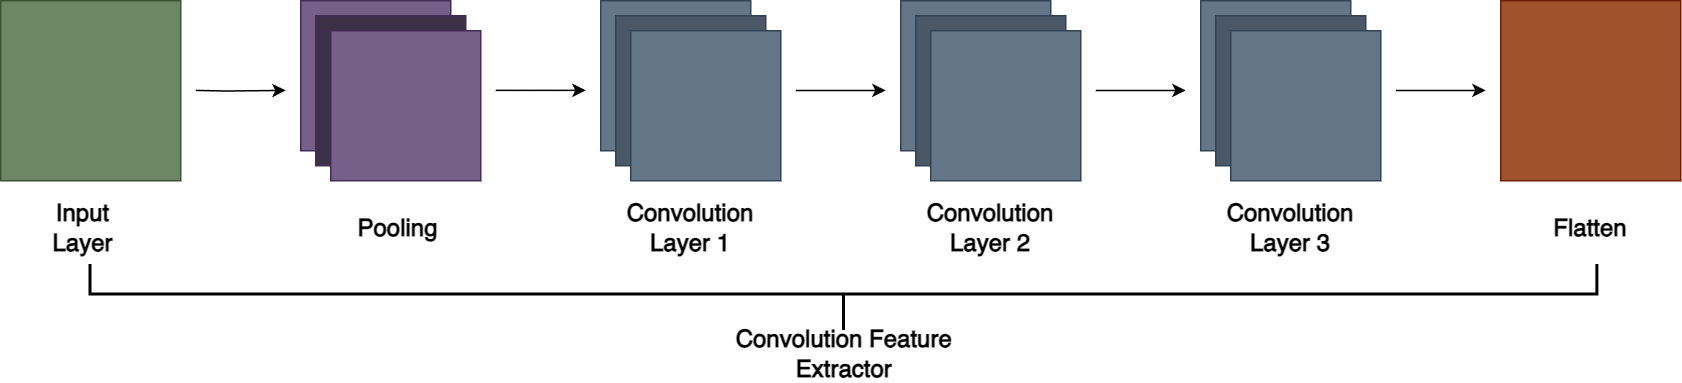
\includegraphics[width=1\textwidth]{images/figureCNN.png}
    \caption{Feature Extraction Block: Input, Convolutional Layers, and Flattening}
    \label{fig:CNN}
\end{figure}

Once flattened, the data is passed through a series of fully connected (dense) layers. Two dense layers are used to interpret the extracted spatial features, with the final hidden layer employing a reduced number of neurons to serve as a decision-making bottleneck. The network concludes with an output layer consisting of two neurons with a linear activation function. These output neurons correspond directly to the vehicle's actuation signals: $y_1$, representing the steering command (normalized steering angle or differential ratio), and $y_2$, representing the throttle or velocity command (normalized pulse-width modulation (PWM) duty cycle).

\begin{figure}[!ht]
    \centering
    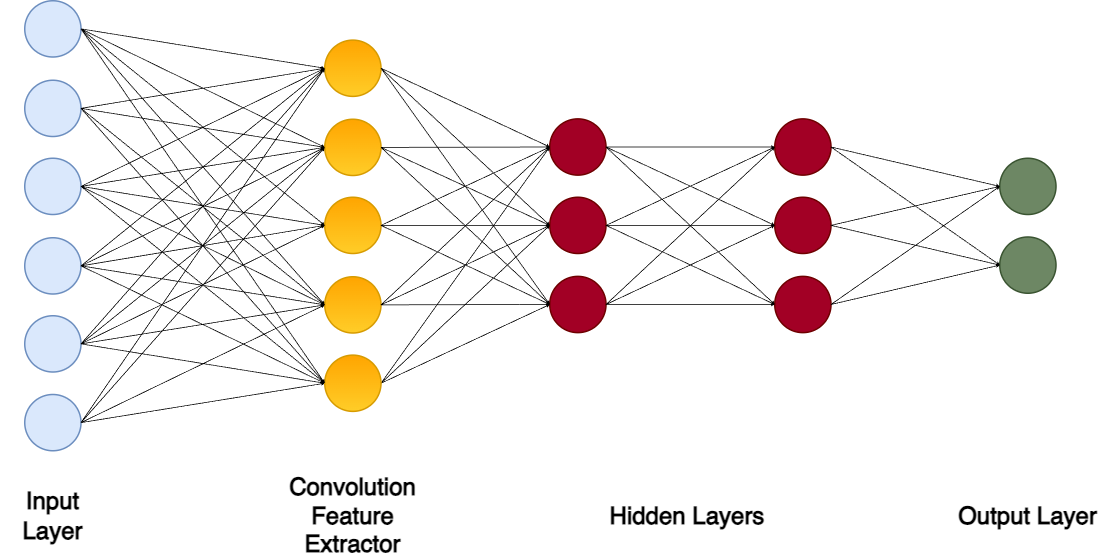
\includegraphics[width=1\linewidth]{images/figure_neural_net.png}
    \caption{Neural Network Diagram: Fully Connected Layers and Actuation Outputs}
    \label{fig:Neural_net}
\end{figure}

\subsection{Input Preprocessing and State Representation}
To ensure the network learns the vehicle's kinematics rather than environmental noise, the raw visual data undergoes rigorous preprocessing based on the homography principles established in Section 2.7.1.

\begin{figure}[!ht]
        \centering
        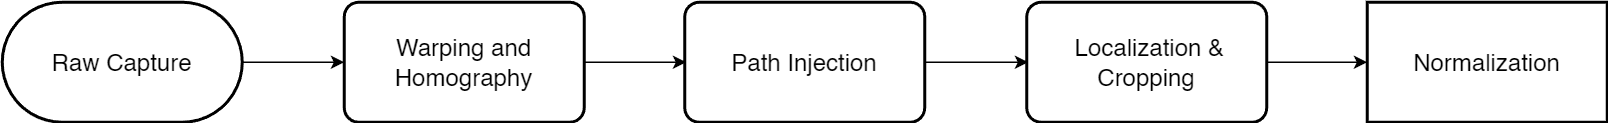
\includegraphics[width=0.9\linewidth]{images/figure_preprocessing.png}
        \caption{The image preprocessing pipeline converting raw camera input into a state representation for the CNN}
        \label{fig:preprocess}
    \end{figure}

\begin{itemize}
    \item \textbf{Homography Transformation:} The raw feed from the overhead camera is warped using the homography matrix $H$, computed via the Direct Linear Transformation (DLT) algorithm. This operation converts the perspective view into a top-down, metric-accurate orthographic representation of the arena.

    \item \textbf{State Augmentation (Path Injection):} To provide the robot with a navigation objective, the target coverage path is digitally rendered onto the transformed image. This results in a composite state representation that encodes both the robot's current pose and the desired trajectory.

    \item \textbf{Region of Interest (ROI) Cropping:} To reduce computational complexity, a fixed-size image crop centered on the robot's coordinates (e.g., $100 \times 100$ pixels) is extracted. This focuses the network on local path-following behavior rather than the full arena context.

    \item \textbf{Normalization:} Pixel intensity values, originally in the integer range $[0,255]$, are normalized to a floating-point range of $[0,1]$ (or $[-1,1]$) to promote numerical stability and faster convergence during gradient-based optimization.
\end{itemize}
\subsection{Data Acquisition and Model Training Pipeline}
Following the Behavioral Cloning paradigm (Section 2.7.3), a dataset will be constructed to capture expert human driving behavior. This study will utilize an Imitation Learning approach, specifically Behavioral Cloning, where the goal is to learn a control policy that mimics expert human driving behavior. The process is divided into two phases: dataset construction and supervised network training. The complete workflow, from the initial capture of human demonstrations to the final optimization of the neural network, is illustrated in \ref{fig:acquisition_training}
\begin{figure}[!ht]
    \centering
    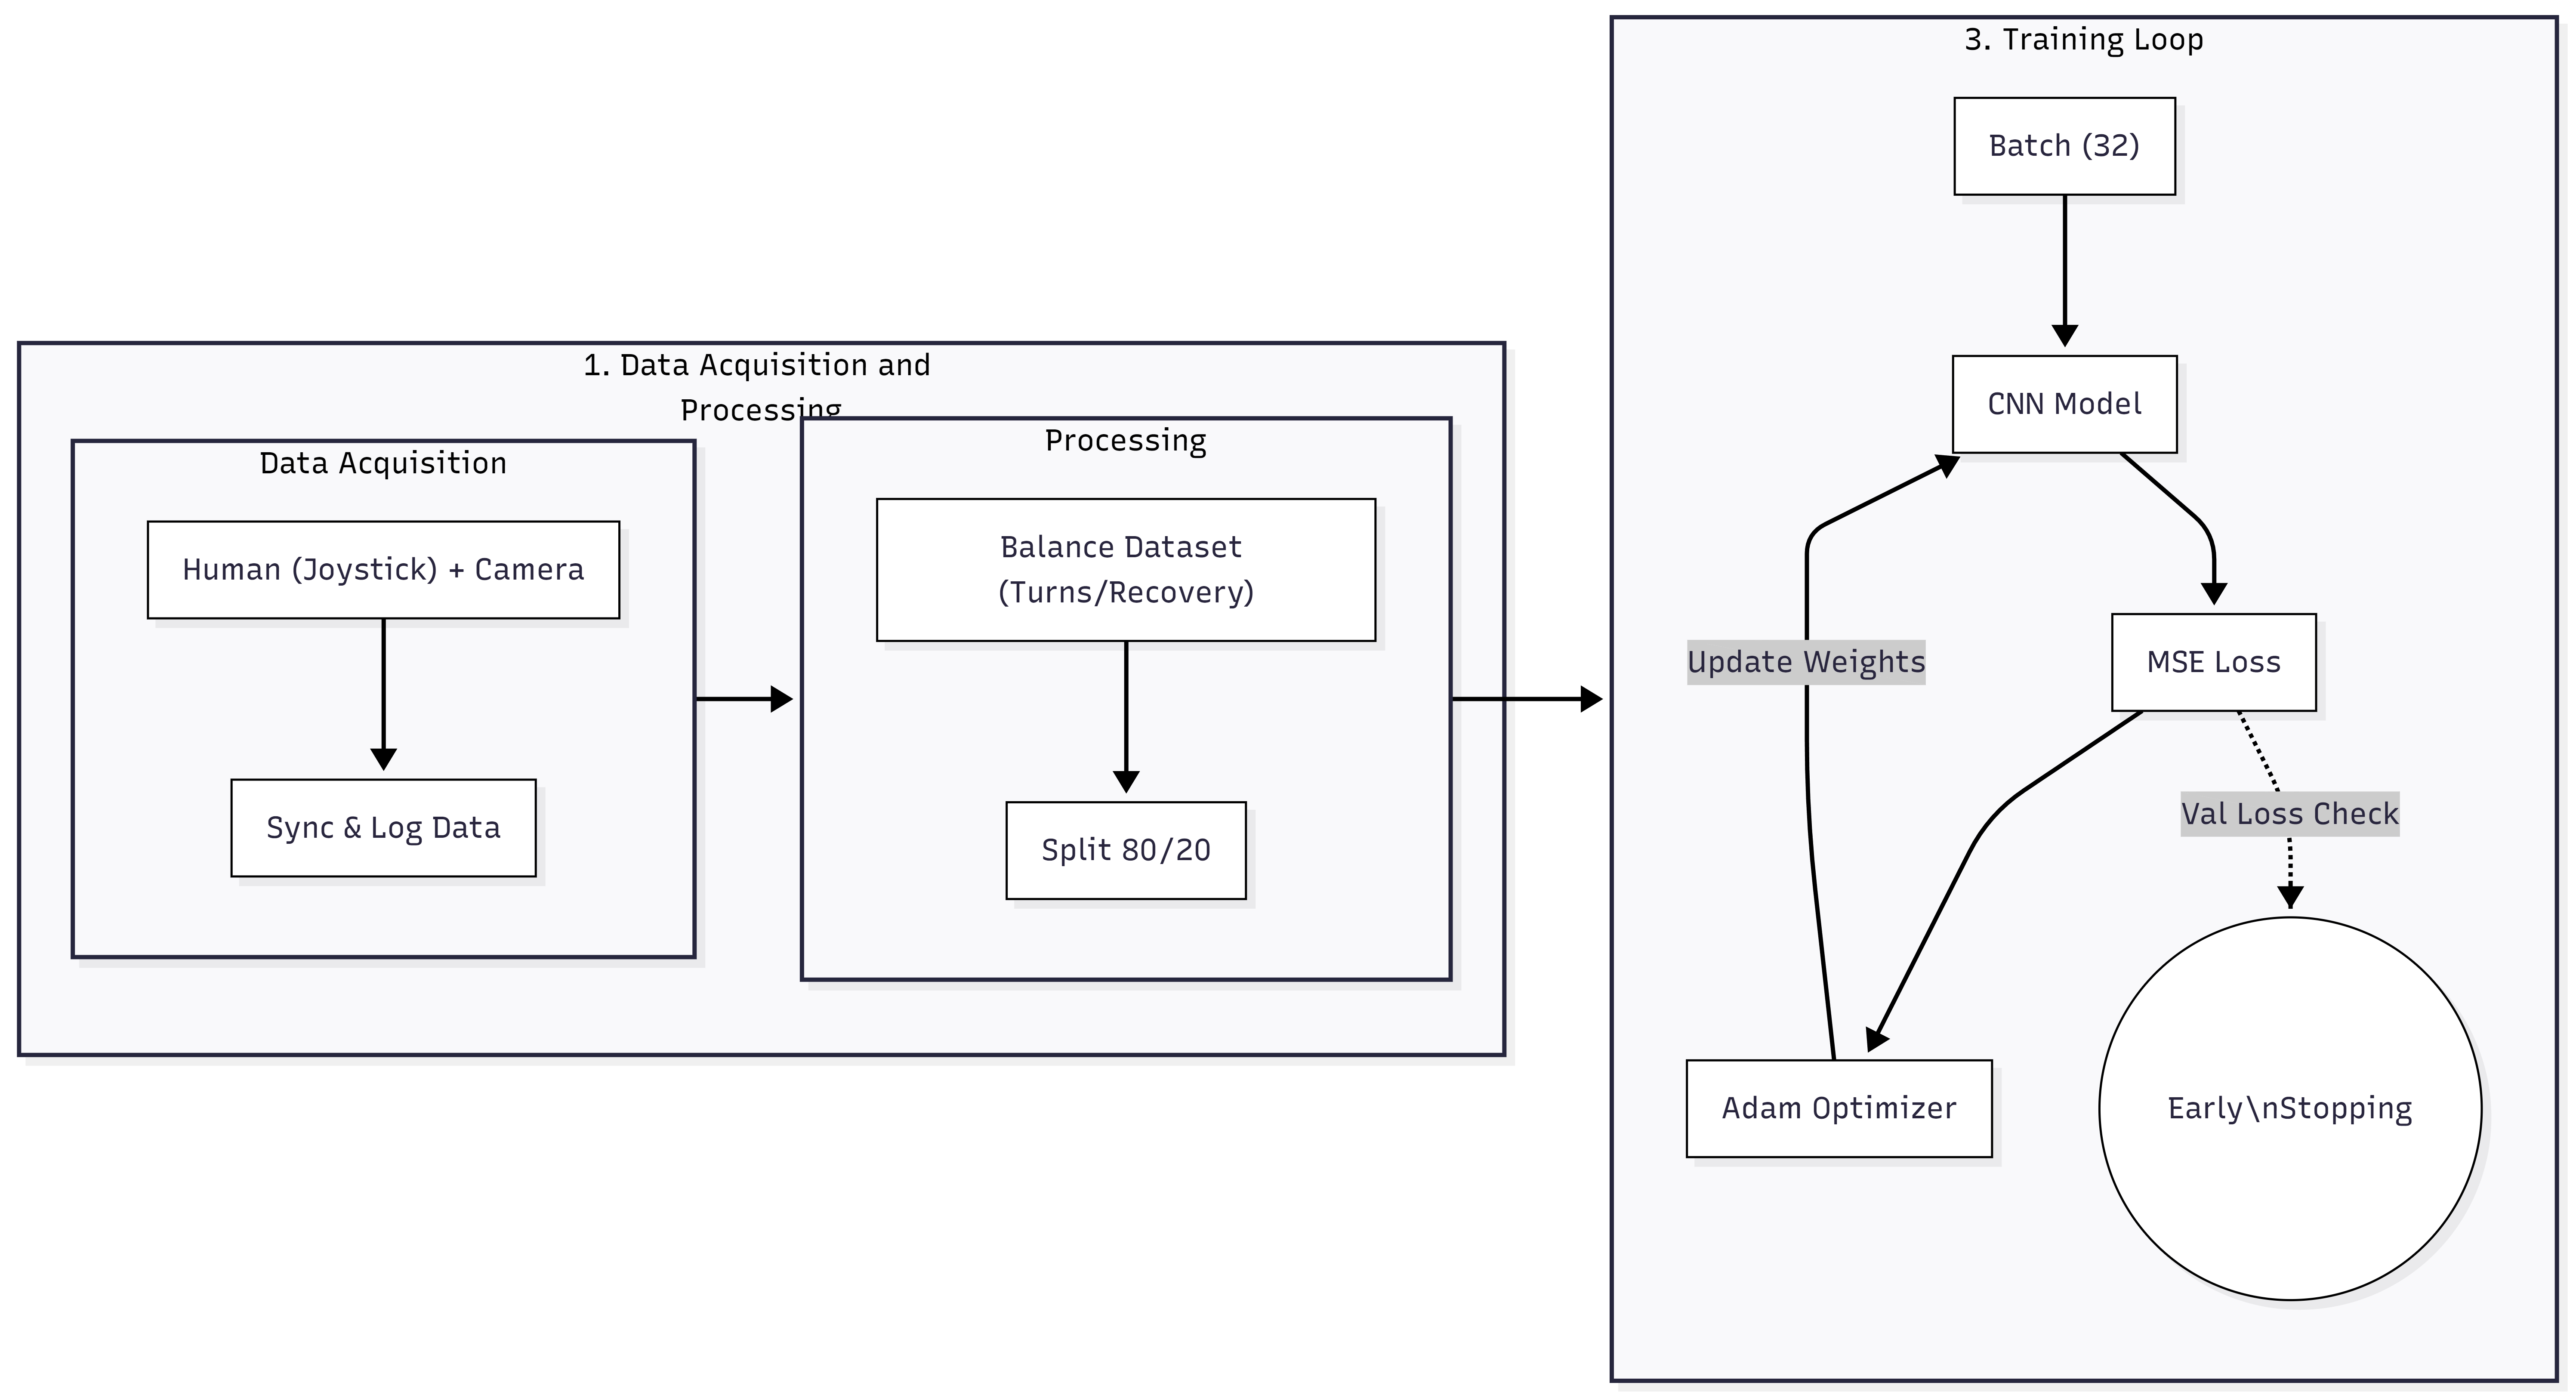
\includegraphics[width=0.7\linewidth]{images/figure_acquisition_training.png}
    \caption{Data Acquisition and Training Pipeline}
    \label{fig:acquisition_training}
\end{figure}

\subsection*{Phase 1: Data Acquisition and Processing}

As shown in the first stage of Figure~3.5, the dataset
\[
\mathcal{D} = \{(s_i, a_i)\}_{i=1}^{N}
\]
is generated by manually controlling the robot using a joystick or gamepad. During these runs, the overhead camera system executes the preprocessing pipeline in real time. A specialized data logger script synchronizes the visual input (state $s_i$) with the human's control inputs (action $a_i$).

\begin{itemize}
    \item \textbf{State ($s_i$):} The preprocessed, cropped image frame.
    \item \textbf{Action ($a_i$):} The control tuple recorded from the joystick.
\end{itemize}

To ensure the model generalizes well and avoids \emph{straight-line bias}, the dataset is balanced to include a diverse distribution of driving scenarios. This explicitly includes straight segments, left and right turns, and recovery maneuvers—instances where the robot is intentionally driven off-path and then corrected—teaching the network how to return to the track center.

\subsection*{Phase 2: Training Configuration}

The network is trained as a regression task using the collected dataset. As depicted in the Training Loop of Figure~3.5, the optimization objective is to minimize the Mean Squared Error (MSE), defined as the Euclidean distance between the predicted control vector and the human’s actual control vector:

\[
\mathcal{L} = \frac{1}{N} \sum_{i=1}^{N}
\left\| y^{(i)}_{\text{pred}} - y^{(i)}_{\text{true}} \right\|^2
\]

The Adam optimizer is selected for its adaptive learning rate capabilities, ensuring stable convergence given the non-convex nature of the loss landscape. An 80:20 dataset split is employed, with 80\% used for training and 20\% for validation. A batch size of 32 is used, and training proceeds until the validation loss plateaus, at which point Early Stopping is applied to prevent overfitting.
\subsection{Deployment and Inference}
\label{sec:deployment_inference}

The trained model is exported and optimized for the target hardware. The deployment process operates in a continuous control loop.

\begin{enumerate}
    \item \textbf{Model Serialization:} The trained network architecture and weights are saved in a portable format (e.g., \texttt{.h5} or \texttt{.tflite}).

    \item \textbf{Inference Loop:} The deployment script runs on the central processing unit (CPU) or the robot’s onboard computer in a continuous loop:
    \begin{enumerate}[\alph*.]
        \item Capture and warp the overhead camera image using the homography transformation.
        \item Preprocess the image and extract the Region of Interest (ROI).
        \item Feed the processed sensor input into the Convolutional Neural Network (CNN).
        \item The CNN outputs raw regression values corresponding to control commands (e.g., steering = 0.3, throttle = 0.8).
        \item The predicted values are scaled to the appropriate PWM range (0--255) and transmitted directly to the motor drivers via GPIO, bypassing any PID or additional error-correction logic.
    \end{enumerate}
\end{enumerate}
% \begin{figure}[!ht]
%     \centering
%     \subbottom[Goku]{
\includegraphics[width=0.3\textwidth]{test_image_goku}}\qquad
%     \subbottom[More Goku]{
\includegraphics[width=0.3\textwidth]{test_image_goku}}%
%     \caption[Short Caption]{The same super saiyan. Two times.}        
%     \label{fig:test2}
% \end{figure}

% Two figures shown side by side are shown in Figure~\ref{fig:test2}.

% \begin{table*}\centering
% \ra{1.3}
% \begin{tabular}{@{}rrrrcrrr@{}}\toprule
% & \multicolumn{3}{c}{$w = 8$} & \phantom{abc}& \multicolumn{3}{c}{$w = 16$} \\
% \cmidrule{2-4} \cmidrule{6-8} 
% & $t=0$ & $t=1$ & $t=2$ && $t=0$ & $t=1$ & $t=2$\\ \midrule
% $dir=1$\\
% $c$ & 0.0790 & 0.1692 & 0.2945 && 0.3670 & 0.7187 & 3.1815\\
% $c$ & -0.8651& 50.0476& 5.9384&& -9.0714& 297.0923& 46.2143\\
% $c$ & 124.2756& -50.9612& -14.2721&& 128.2265& -630.5455& -381.0930\\
% $dir=0$\\
% $c$ & 0.0357& 1.2473& 0.2119&& 0.3593& -0.2755& 2.1764\\
% $c$ & -17.9048& -37.1111& 8.8591&& -30.7381& -9.5952& -3.0000\\
% $c$ & 105.5518& 232.1160& -94.7351&& 100.2497& 141.2778& -259.7326\\
% \bottomrule
% \end{tabular}
% \caption{A Beautiful and Complex Table}\label{tab:sometable}
% \end{table*}
\section{Software Architecture}

This section details the software framework governing the autonomous vehicle. The system is designed as a modular, monolithic application primarily implemented in Python, leveraging libraries such as OpenCV for computer vision and TensorFlow/PyTorch for deep learning inference. The architecture prioritizes low latency to ensure the end-to-end control loop maintains a sufficient frequency for stable navigation.

\subsection{Module Integration}
\label{sec:module_integration}

The software is organized into four distinct functional modules. This modular design ensures separation of concerns, allowing for easier debugging and independent testing of subsystems (e.g., testing image warping without running the motors). The core modules are defined as follows:

\begin{enumerate}
    \item \textbf{Perception Interface (\textit{CameraStream}):}
    \begin{itemize}
        \item Responsible for interfacing with the hardware camera driver.
        \item Manages the frame buffer to ensure the processing pipeline always retrieves the most recent frame, discarding stale data to minimize input lag.
    \end{itemize}

    \item \textbf{State Estimator (\textit{Preprocessor}):}
    \begin{itemize}
        \item Encapsulates the geometric logic described in Section~3.4.
        \item Contains the pre-calculated homography matrix $H$ and performs the perspective warp and ROI cropping.
        \item Handles the normalization of pixel values before passing sensor data to the neural network.
    \end{itemize}

    \item \textbf{Inference Engine (\textit{PilotModel}):}
    \begin{itemize}
        \item Loads the pre-trained CNN model weights into memory during initialization.
        \item Provides a \texttt{predict()} method that accepts the processed image tensor and returns the raw steering and throttle outputs.
        \item Is optimized to run on the specific hardware accelerator (e.g., GPU or Neural Processing Unit), if available.
    \end{itemize}

    \item \textbf{Actuation Interface (\textit{MotorDriver}):}
    \begin{itemize}
        \item Abstracts the low-level GPIO (General Purpose Input/Output) commands.
        \item Converts the normalized CNN output (e.g., $[-1,1]$ or $[0,1]$) into hardware-specific PWM duty cycles (e.g., 0--255 or 0--65535).
        \item Includes safety stops, ensuring the motors default to zero velocity if the software is interrupted.
    \end{itemize}
\end{enumerate}
\begin{algorithm}[H]
\caption{Homography Estimation and Perspective Warping}
\label{alg:homography_warping}
\begin{algorithmic}[1]

\Function{InitializeAndWarp}{$raw\_frame, camera\_matrix, dist\_coeffs, arena\_dims$}
\State \textbf{Input:}
\State \hspace{1em} $raw\_frame$ — Raw RGB image from the camera
\State \hspace{1em} $camera\_matrix (K), dist\_coeffs (D)$ — Intrinsic calibration parameters
\State \hspace{1em} $arena\_dims$ — Target width and height of bird's-eye view
\State \textbf{Output:} $warped\_frame, homography\_matrix$

\Statex
\State \textbf{// Phase 1: Undistortion}
\State $undistorted\_frame \gets \textsc{Undistort}(raw\_frame, K, D)$
\State $gray\_frame \gets \textsc{ConvertToGray}(undistorted\_frame)$

\Statex
\State \textbf{// Phase 2: Marker Detection}
\State $dictionary \gets \textsc{GetDictionary}(\texttt{DICT\_4X4\_50})$
\State $(corners, ids) \gets \textsc{DetectMarkers}(gray\_frame, dictionary)$

\Statex
\State \textbf{// Phase 3: ID-Based Sorting (Ground Truth Assignment)}
\State \textbf{// Marker IDs: 0=TL, 1=TR, 2=BR, 3=BL}
\State $expected\_ids \gets \{0,1,2,3\}$

\If{$|ids| < 4$ \textbf{or} $expected\_ids \not\subseteq ids$}
    \State \Return \textbf{Error} ``Markers 0--3 not found''
\EndIf

\State $src\_points \gets$ empty list of size $4$

\For{$i \gets 1$ to $|ids|$}
    \If{$ids[i] = 0$}
        \State $src\_points[0] \gets corners[i]$ \Comment{Top-Left}
    \ElsIf{$ids[i] = 1$}
        \State $src\_points[1] \gets corners[i]$ \Comment{Top-Right}
    \ElsIf{$ids[i] = 2$}
        \State $src\_points[2] \gets corners[i]$ \Comment{Bottom-Right}
    \ElsIf{$ids[i] = 3$}
        \State $src\_points[3] \gets corners[i]$ \Comment{Bottom-Left}
    \EndIf
\EndFor

\Statex
\State \textbf{// Phase 4: Homography Calculation}
\State $dst\_points \gets \{(0,0), (W,0), (W,H), (0,H)\}$
\State $homography\_matrix \gets \textsc{GetPerspectiveTransform}(src\_points, dst\_points)$

\Statex
\State \textbf{// Phase 5: Perspective Warping}
\State $warped\_frame \gets \textsc{WarpPerspective}(undistorted\_frame, homography\_matrix, arena\_dims)$

\State \Return $warped\_frame, homography\_matrix$
\EndFunction

\end{algorithmic}
\end{algorithm}

\begin{algorithm}[H]
\caption{Navigation Agent: Neural Network Inference}
\label{alg:inference_logic}
\begin{algorithmic}[1]

\Function{ComputeControlVector}{$warped\_frame, cnn\_model$}
    \State \textbf{Input:} Top-down image and pre-trained CNN model
    \State \textbf{Output:} Steering angle and throttle commands

    \Statex
    \State \textbf{// Step 1: Pre-processing}
    \State $input \gets \textsc{Resize}(warped\_frame, 66 \times 200)$
    \State $input \gets \textsc{NormalizePixelValues}(input)$ \Comment{Scale to range [0, 1]}

    \Statex
    \State \textbf{// Step 2: Deep Learning Inference}
    \State $(raw\_steer, raw\_throttle) \gets \textsc{ModelPredict}(cnn\_model, input)$

    \Statex
    \State \textbf{// Step 3: Safety Saturation}
    \State \Comment{Clip outputs to ensure values are within hardware limits}
    \State $steering \gets \textsc{Clip}(raw\_steer, -1.0, 1.0)$
    \State $throttle \gets \textsc{Clip}(raw\_throttle, 0.0, 1.0)$

    \State \Return $steering, throttle$
\EndFunction

\end{algorithmic}
\end{algorithm}

\begin{algorithm}[H]
\caption{Actuation: Hardware Control Interface}
\label{alg:actuation_logic}
\begin{algorithmic}[1]

\Function{DriveRobot}{$steering, throttle$}
    \State \textbf{Input:} Normalized control commands from Neural Network
    \State \textbf{Output:} Physical electrical signals to motors

    \Statex
    \State \textbf{// Step 1: Safety Check}
    \If{Watchdog Timer Expired}
        \State \textsc{TriggerEmergencyStop}()
        \State \Return
    \EndIf

    \Statex
    \State \textbf{// Step 2: Signal Conversion}
    \State \Comment{Convert normalized values to Pulse Width Modulation (PWM)}
    \State $servo\_signal \gets \textsc{MapToServoDutyCycle}(steering)$
    \State $motor\_signal \gets \textsc{MapToDCMotorSpeed}(throttle)$

    \Statex
    \State \textbf{// Step 3: Hardware Execution}
    \State \textsc{WriteGPIO}(SERVO\_PIN, $servo\_signal$)
    \State \textsc{WriteGPIO}(MOTOR\_PIN, $motor\_signal$)

\EndFunction

\end{algorithmic}
\end{algorithm}

\subsection{Real-Time Execution and Middleware}
\label{sec:realtime_execution}

The system operates using a synchronous main control loop. Unlike asynchronous systems that rely on complex middleware (e.g., ROS) for message passing, this study utilizes a direct memory access approach to minimize overhead and latency. This design choice is critical for achieving stable end-to-end controller without PID dampening.

\subsubsection*{Execution Flow}
The main execution pipeline follows a ``Sense-Think-Act'' cycle:

\begin{enumerate}
    \item \textbf{Initialization Phase:} On startup, the system verifies hardware connections, warms up the camera sensor (allowing auto-exposure to settle), and loads the CNN model into RAM.
    \item \textbf{The Control Loop:} The system enters a \texttt{while(true)} loop that executes the following sequence:
    \begin{itemize}
        \item Acquire: The \texttt{CameraStream} fetches the latest frame.
        \item Process: The \texttt{Preprocessor} warps and crops the image.
        \item Infer: The \texttt{PilotModel} computes the control vector.
        \item Drive: The \texttt{MotorDriver} executes the command.
        \item Log: (Optional) Data is saved for debugging or further training.
    \end{itemize}
\end{enumerate}

\subsubsection*{Timing and Latency}
To maintain smooth motion, the software is designed to run at a target frequency of 15Hz to 20Hz. The most computationally expensive step is the CNN inference; therefore, the input image resolution is kept minimal to mitigate latency. A software watchdog is implemented to monitor the loop time; if the camera disconnects or the loop hangs, the actuation interface triggers a safety stop to prevent runaway behavior.

\section{Evaluation and Testing}
To rigorously assess the performance of the end-to-end CNN controller, a series of controlled experiments were designed. These tests aim to quantify the system's ability to track a digitally rendered path using only visual inputs, without the assistance of heuristic algorithms or PID feedback loops.

\subsection{Evaluation Scenarios}
The system will be tested across three track configurations, each designed to isolate specific driving behaviors and failure nodes. All tests will be conducted in a controlled indoor environment with constant lighting conditions to minimize perception noise. The first scenario will consist of a straightforward path. The primary objective will be to evaluate the system's stability and its ability to maintain a straight heading without oscillations, a common issue we might experience with behavioral cloning models lacking a derivative term. The second scenario will feature a track with multiple 90-degree turns and a U-turn. This scenario will test the system's ability to anticipate sharp changes in curvature and modulate the throttle as will be learned from the human demonstration data. As for the last scenario, the robot will intentionally be initialized at an offset position and with a misaligned heading. This test will evaluate the generalization capability of the model, specifically whether it could recover and return to the path center, a behavior that must be learned from the recovery examples in the training dataset.
\begin{figure}[!ht]
    \centering
    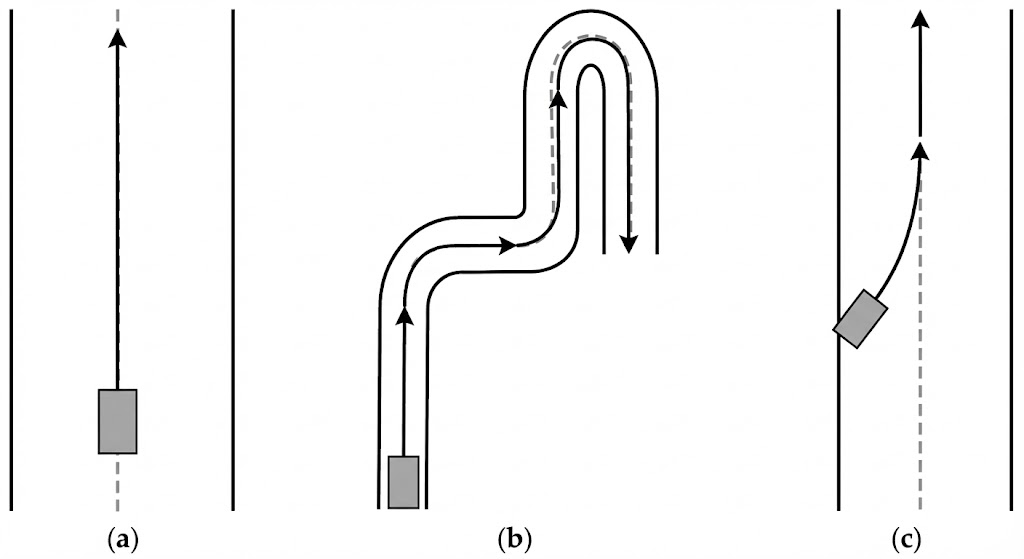
\includegraphics[width=1\linewidth]{figure_Eval_Scenarios.png}
    \caption{Schematic representation of the three experimental track configurations. (a) Scenario 1 tests straight-line stability on a straightforward path. (b) Scenario 2 evaluates the system's ability to handle sharp curvatures using 90-degree turns and a U-turn. (c) Scenario 3 tests generalization capability by initializing the robot with an offset position and misaligned heading, requiring it to recover to the path center.}
    \label{fig:testing_scenarios}
\end{figure}
\subsection{Performance Metrics}

To objectively quantify the navigation performance of the end-to-end controller, the study will utilize four primary metrics derived from the ground truth data captured by the overhead tracking system. The fundamental measure of tracking accuracy will be the Cross-Track Error (CTE). This is defined as the perpendicular distance between the robot's geometric center and the nearest point on the digital reference path at any given time step $t$. To provide a summary statistic for the entire run, the study will calculate the Root Mean Square Error (RMSE) of these deviations. A lower RMSE would indicate a tighter adherence to the reference path.
\begin{figure}[!ht]
    \centering
    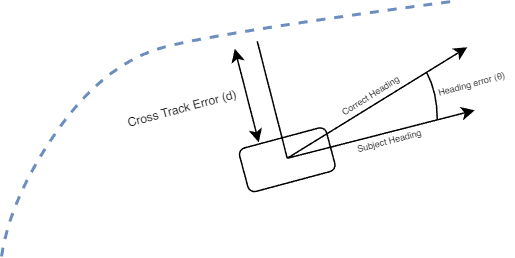
\includegraphics[width=0.8\linewidth]{images/figure_track_error.png}
    \caption{Visual Representation of Cross Track Error ($d$) and Heading Error ($\theta$).}
    \label{fig:cte_heading_error}
\end{figure}

Complementing the position error is the Heading Error, which evaluates the robot's orientation accuracy. This metric measures the angular difference between the robot's current yaw angle ($\theta_{robot}$) and the tangent angle of the path ($\theta_{path}$) at the nearest point. Monitoring heading error is critical for predictive analysis, as high angular deviations often precede a complete departure from the lane. Finally, the overall reliability of the system will be measured by the \textbf{Success Rate}, a qualitative metric calculated as the percentage of total attempts where the robot completed the entire course without any part of its chassis crossing the lane boundaries.
    \chapter{Results \& Discussion}
This chapter presents the evaluation of the developed end-to-end autonomous navigation system. The results are presented chronologically, tracing the system's iterative development. All physical deployment and inference runs reported in this chapter were executed on the real robot, with the trained model running onboard a Raspberry Pi embedded on the platform.

To validate the necessity of the final image preprocessing architecture, the chapter first details the offline training and real-world physical testing of two early experimental baselines. By analyzing the specific failure modes of these early iterations, the empirical justification for the proposed Egocentric Dynamic Crop Model is established.


\section{Chronological Development and Experimental Baselines}
During the development of the navigation framework, the state representation of the track underwent three major iterations. All models were trained using a modified NVIDIA DAVE-2 Convolutional Neural Network (CNN) architecture with 2,211,175 parameters, processing $200 \times 200$ pixel images, and minimizing Mean Squared Error (MSE) using the Adam optimizer.

\subsection{Iteration 1: Baseline A (Allocentric Full AOI Model)}
The initial approach utilized the raw, top-down Bird's-Eye View (BEV) image, retaining the room's floor textures and permanent background elements.

During offline training, Baseline A converged rapidly. As shown in Figure~\ref{fig:4.1}, both MSE and MAE decreased exponentially, with validation loss plateauing near 0.05 and 0.13, and reaching a low validation MSE of 0.0489 by Epoch 30.

% [Insert Figure 4.1: Baseline A (Allocentric Full AOI) Offline Training and Validation Loss Curves]
\begin{figure}[htbp]
	\centering
	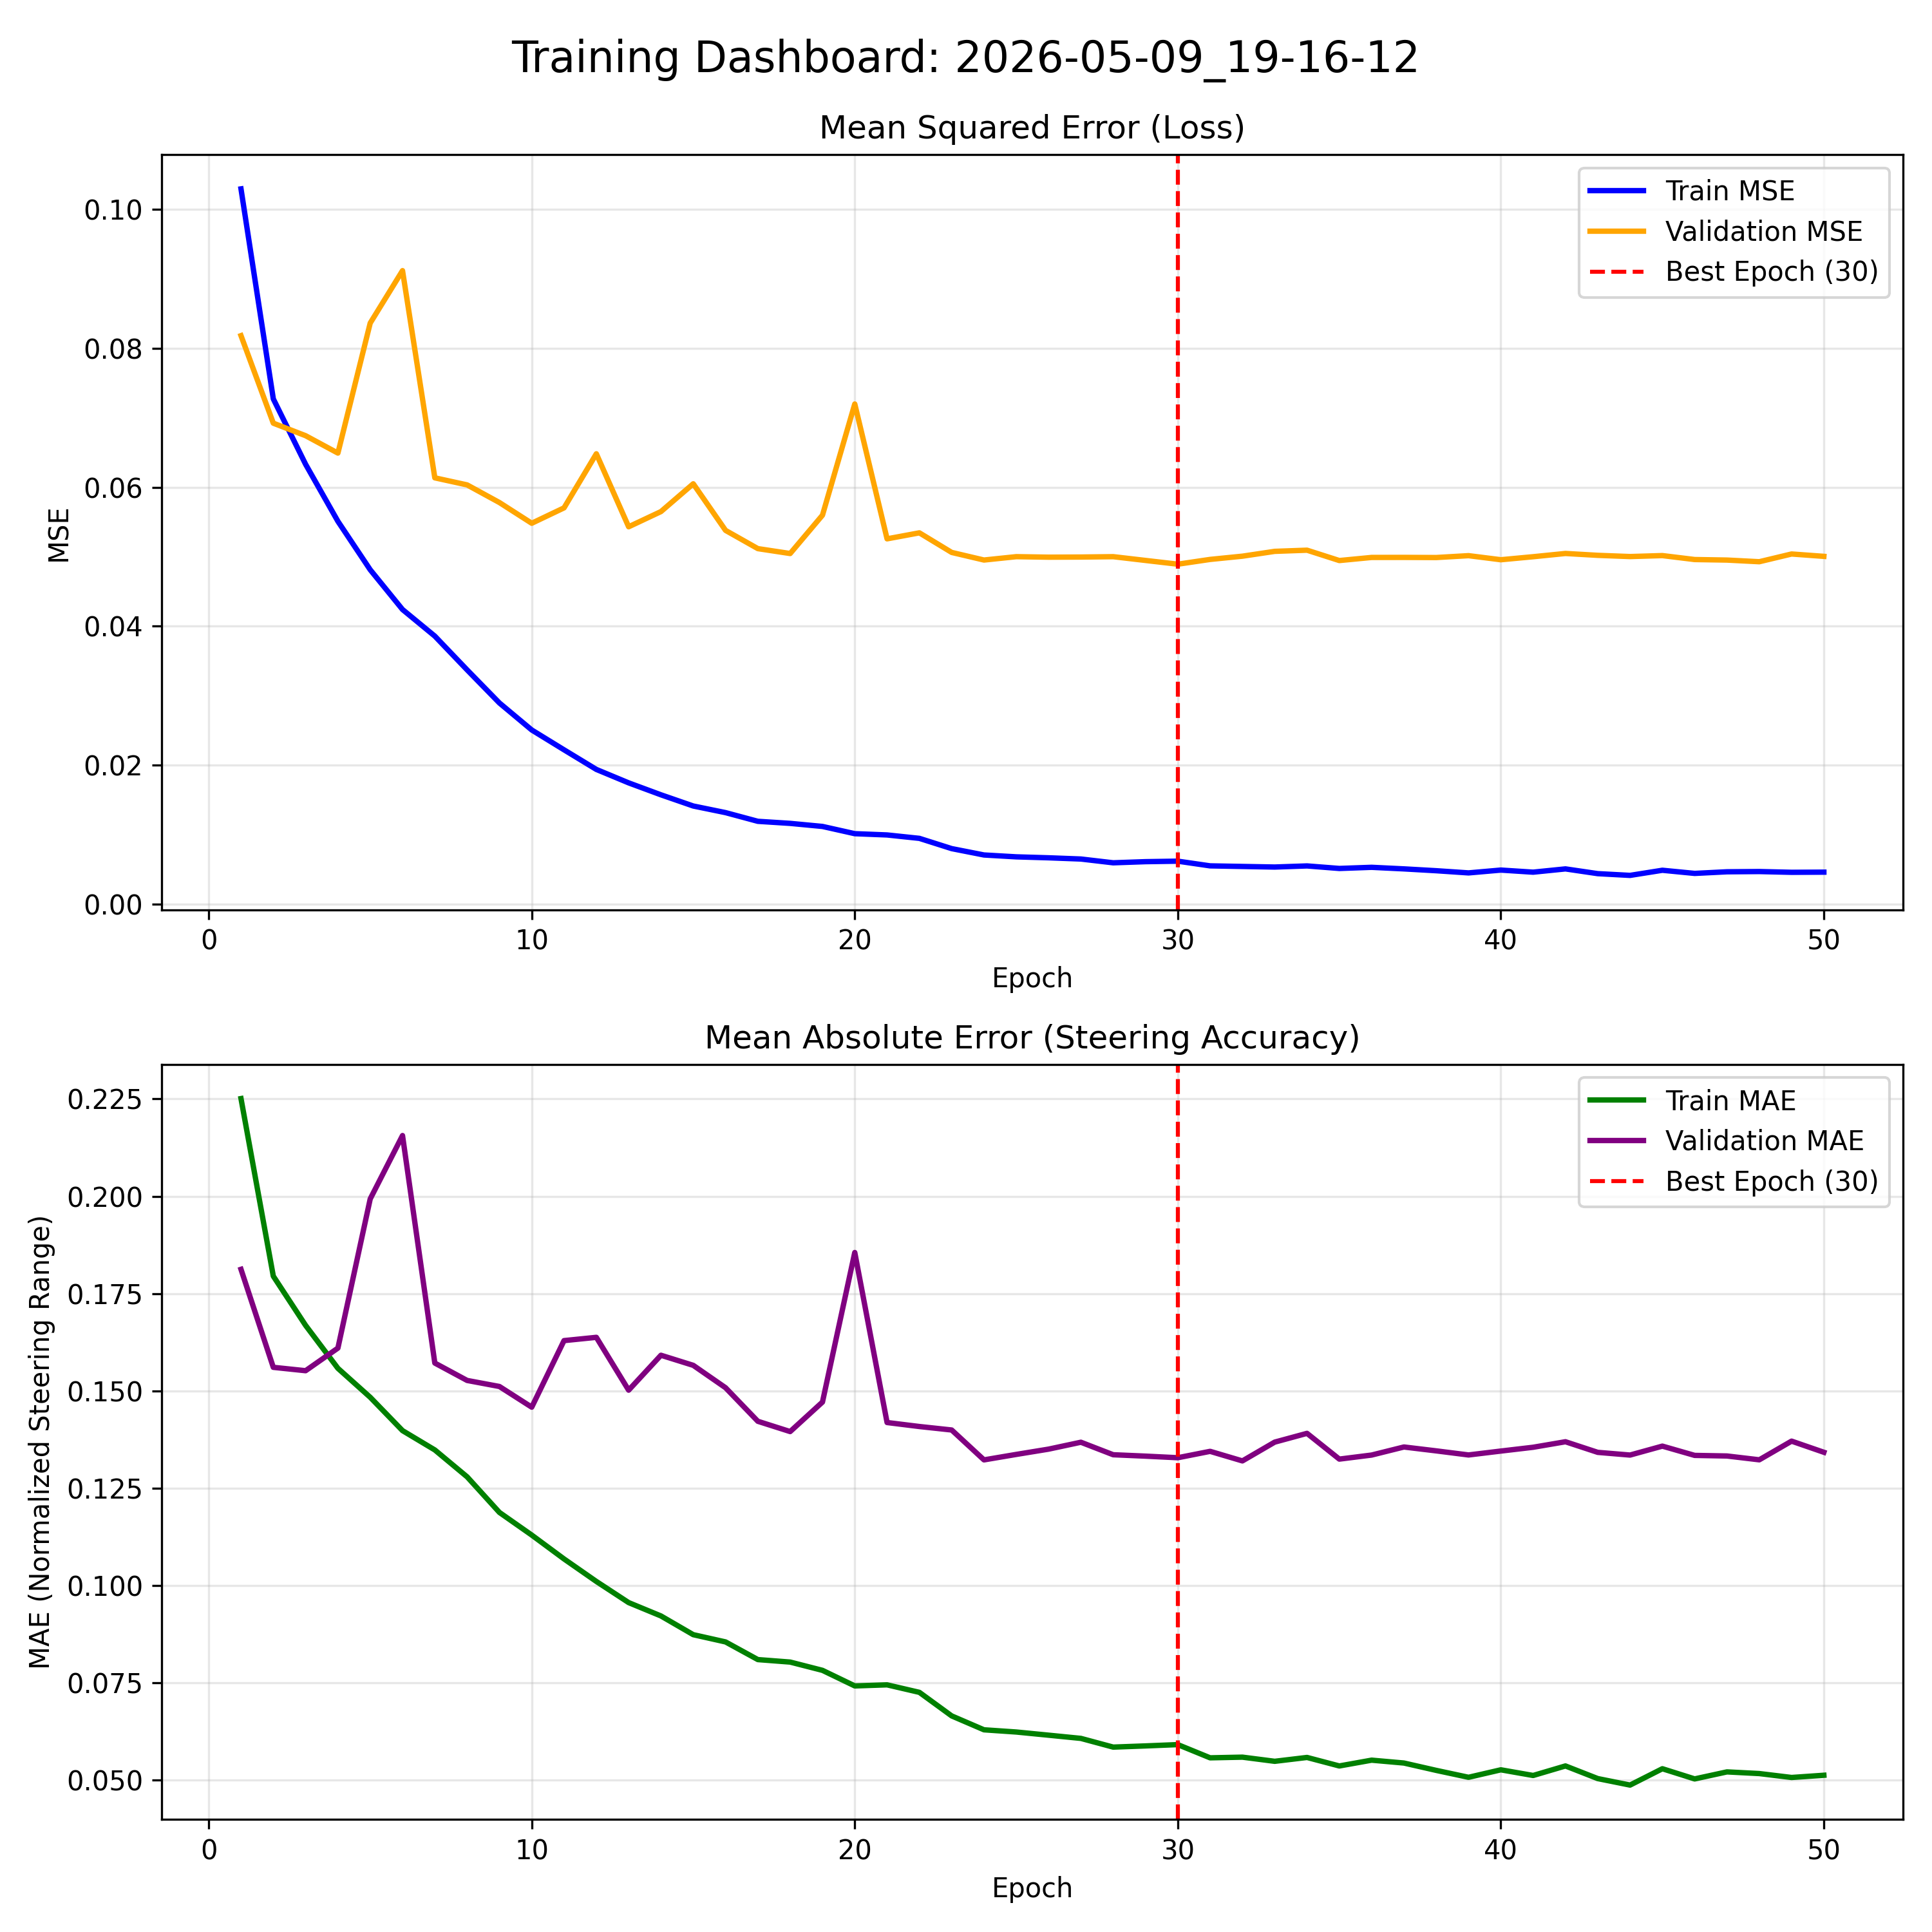
\includegraphics[width=1\linewidth]{chap4/images/2nd_session.png}
	\caption{The near-perfect convergence of MSE and MAE suggested successful learning, though this was later identified as spatial memorization.}\label{fig:4.1}
\end{figure}

However, physical deployment resulted in immediate, catastrophic navigation failure. On the physical track, the robot exhibited erratic motor control, immediately veering off-path and breaching the arena boundaries.

\begin{figure}[htbp]
	\centering
	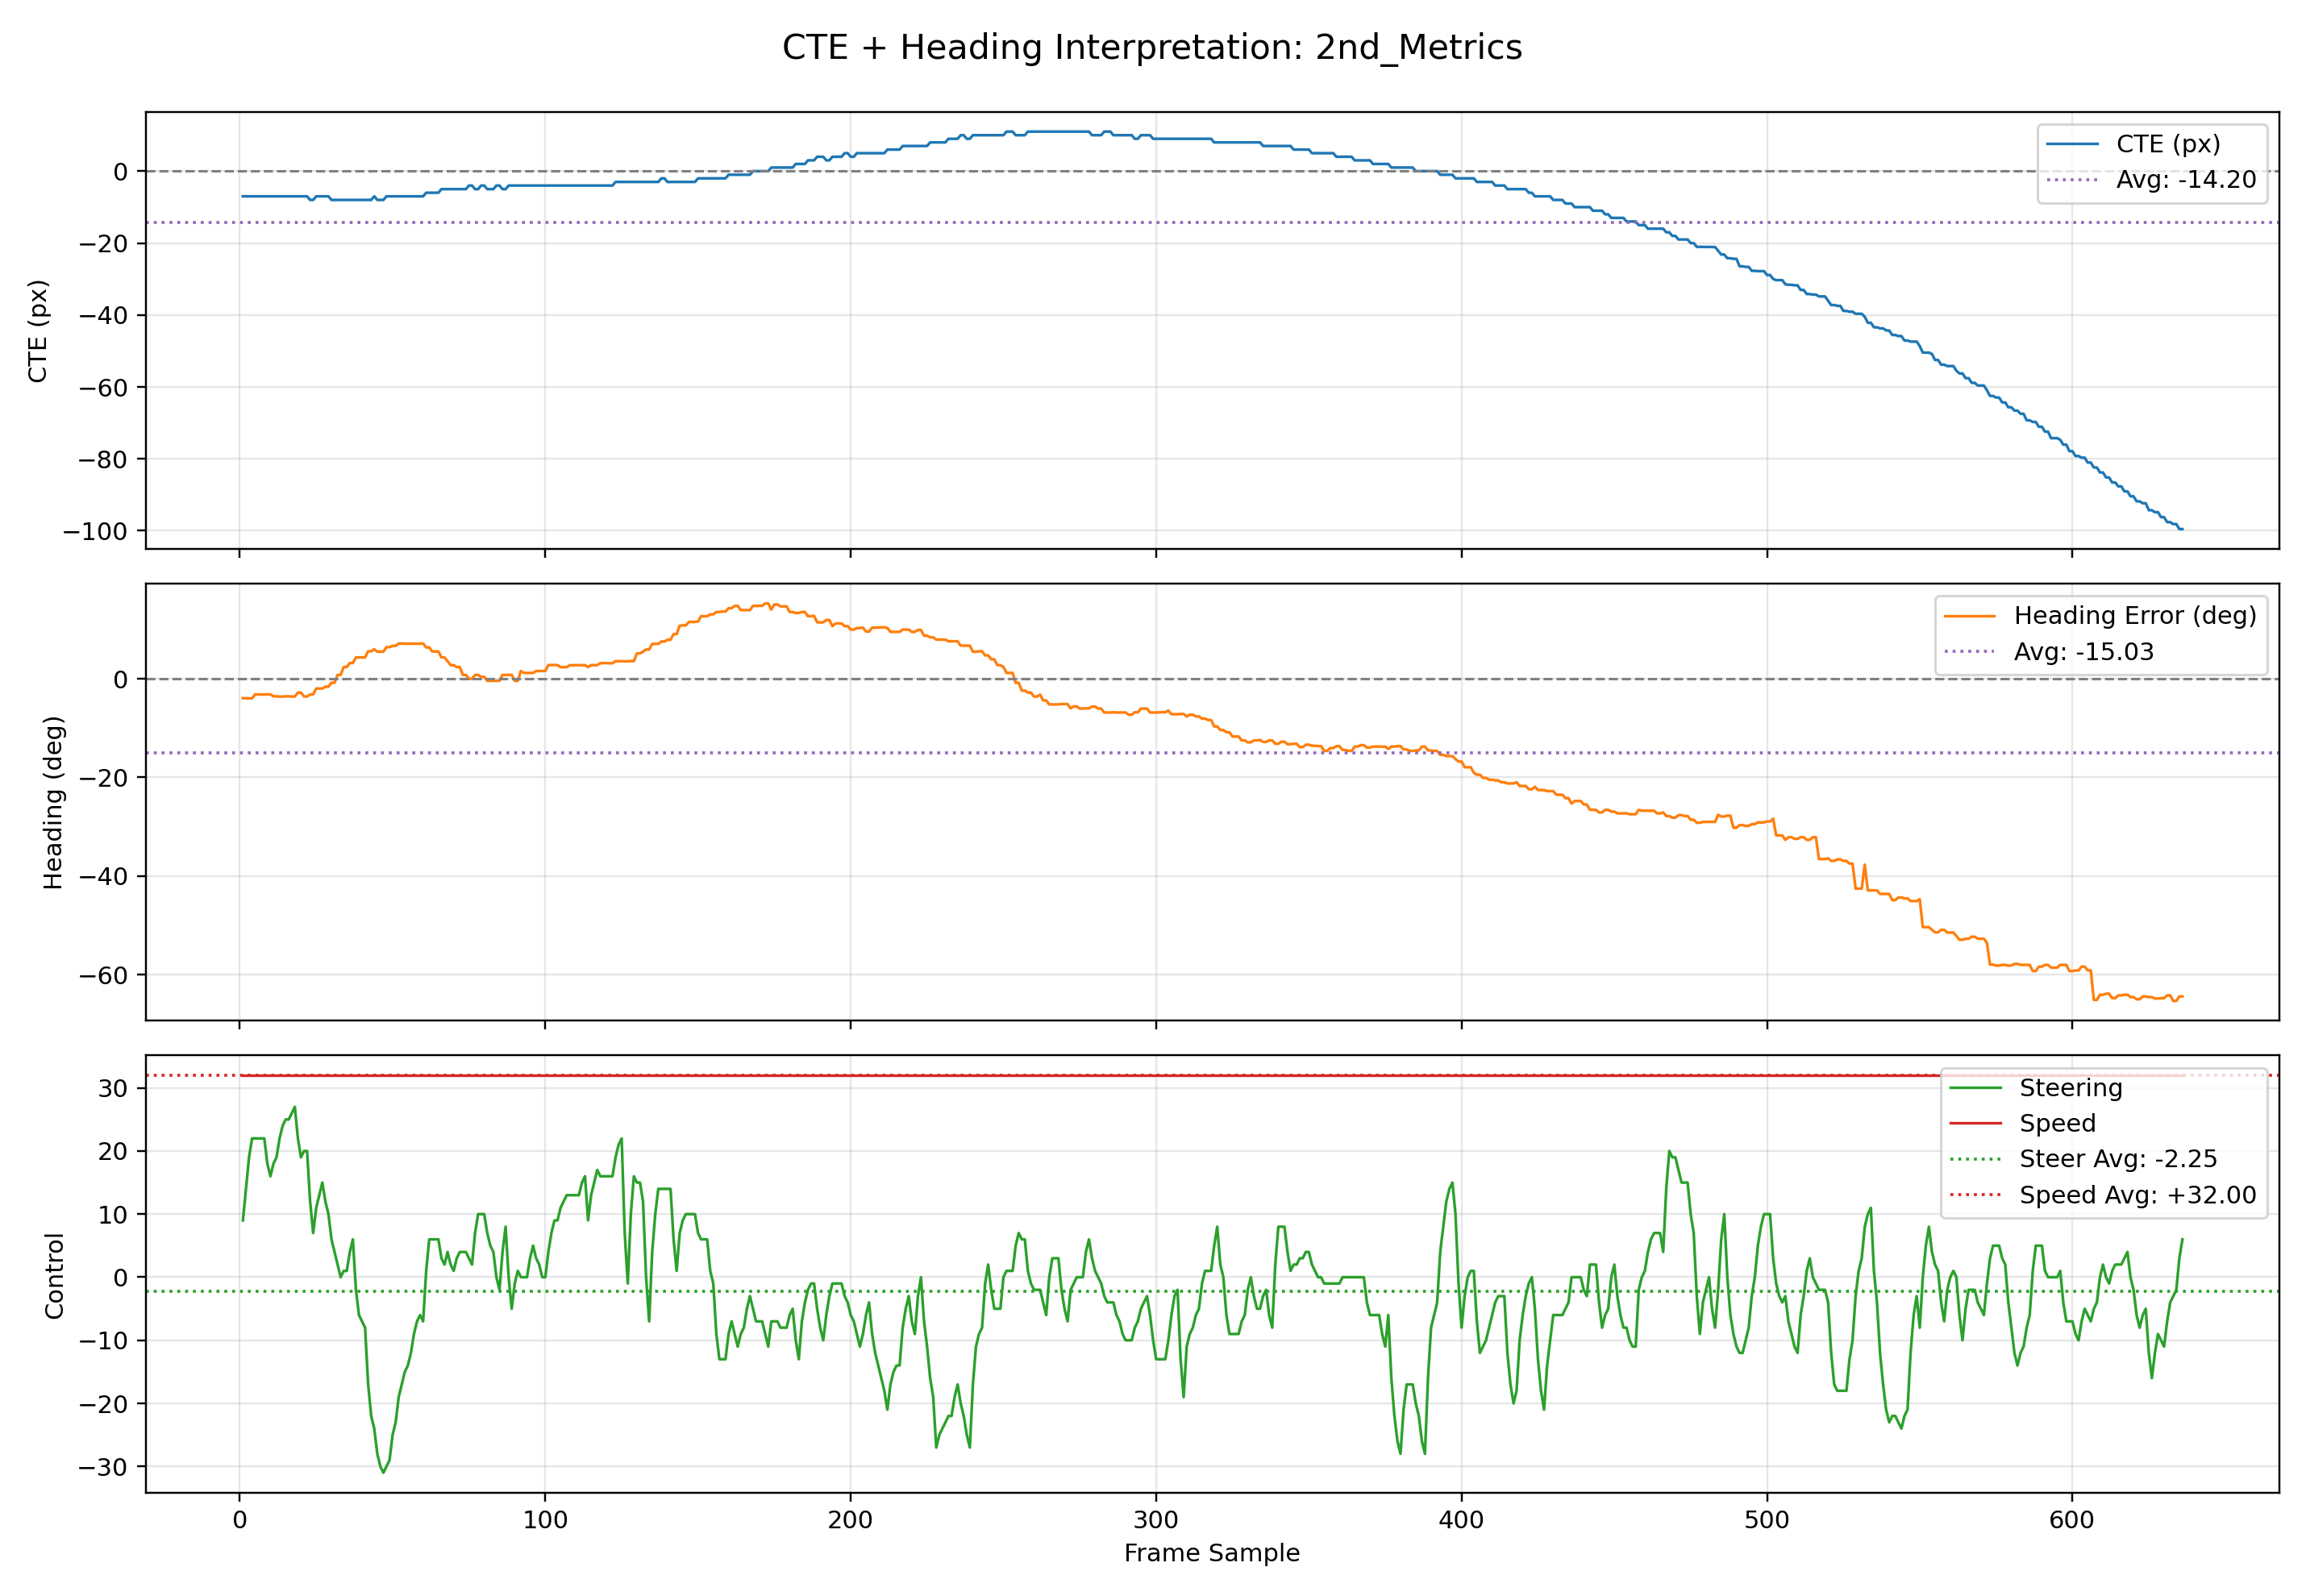
\includegraphics[width=1.0\linewidth]{chap4/images/2nd_Metrics_interpretation.png}
	\caption{Physical deployment of the Allocentric Full AOI Model resulted in immediate navigation failure.}\label{fig:4.2}
\end{figure}

As shown in Figure~\ref{fig:4.2}, both the Cross-Track Error (CTE) and the Heading Error ($\theta_{err}$) diverged immediately on deployment (CTE quickly exceeding $-100$ pixels and Heading Error dropping past $-60^\circ$). Baseline A maintained the path for only 636 frames with an RMSE of 30.9992 pixels. When analyzing the Error Compounding Rate over the first 500 frames, Baseline A showed rapid, exponential error growth. Minor starting position changes on the real track confused the network, causing it to immediately steer off course.

Post-deployment analysis revealed the model suffered from \textbf{shortcut learning}. Because the room environment and global track remained static in the camera's view, the CNN bypassed learning the path geometry entirely. Instead, it overfit directly to the robot's absolute pixel coordinates within the room frame. The validation error remained low during training because validation images came from that same static frame. During inference, any minor starting deviation created an out-of-distribution pixel state that the model could not interpret.

\subsection{Iteration 2: Baseline B (Feature-Extracted Allocentric Model)}
To eliminate background shortcuts like floor reflections, shadows, and pixel discrepancies, the pipeline was updated to add a semantic polygon extraction step. This process isolated the AOI as flat white shapes with a red polygon on a pure black canvas, removing all environmental noise and forcing the network to learn the path geometry itself.

While this removed environmental noise, offline training metrics immediately destabilized. As shown in Figure~\ref{fig:4.3}, the training profile exhibited severe validation noise and a massive loss spike near epoch 13, indicating the network struggled to map steering angles without its familiar background shortcuts. The resulting controller was not stable enough to justify full physical deployment, and the model was therefore not advanced beyond limited sanity checks.


\begin{figure}[H]
	\centering
	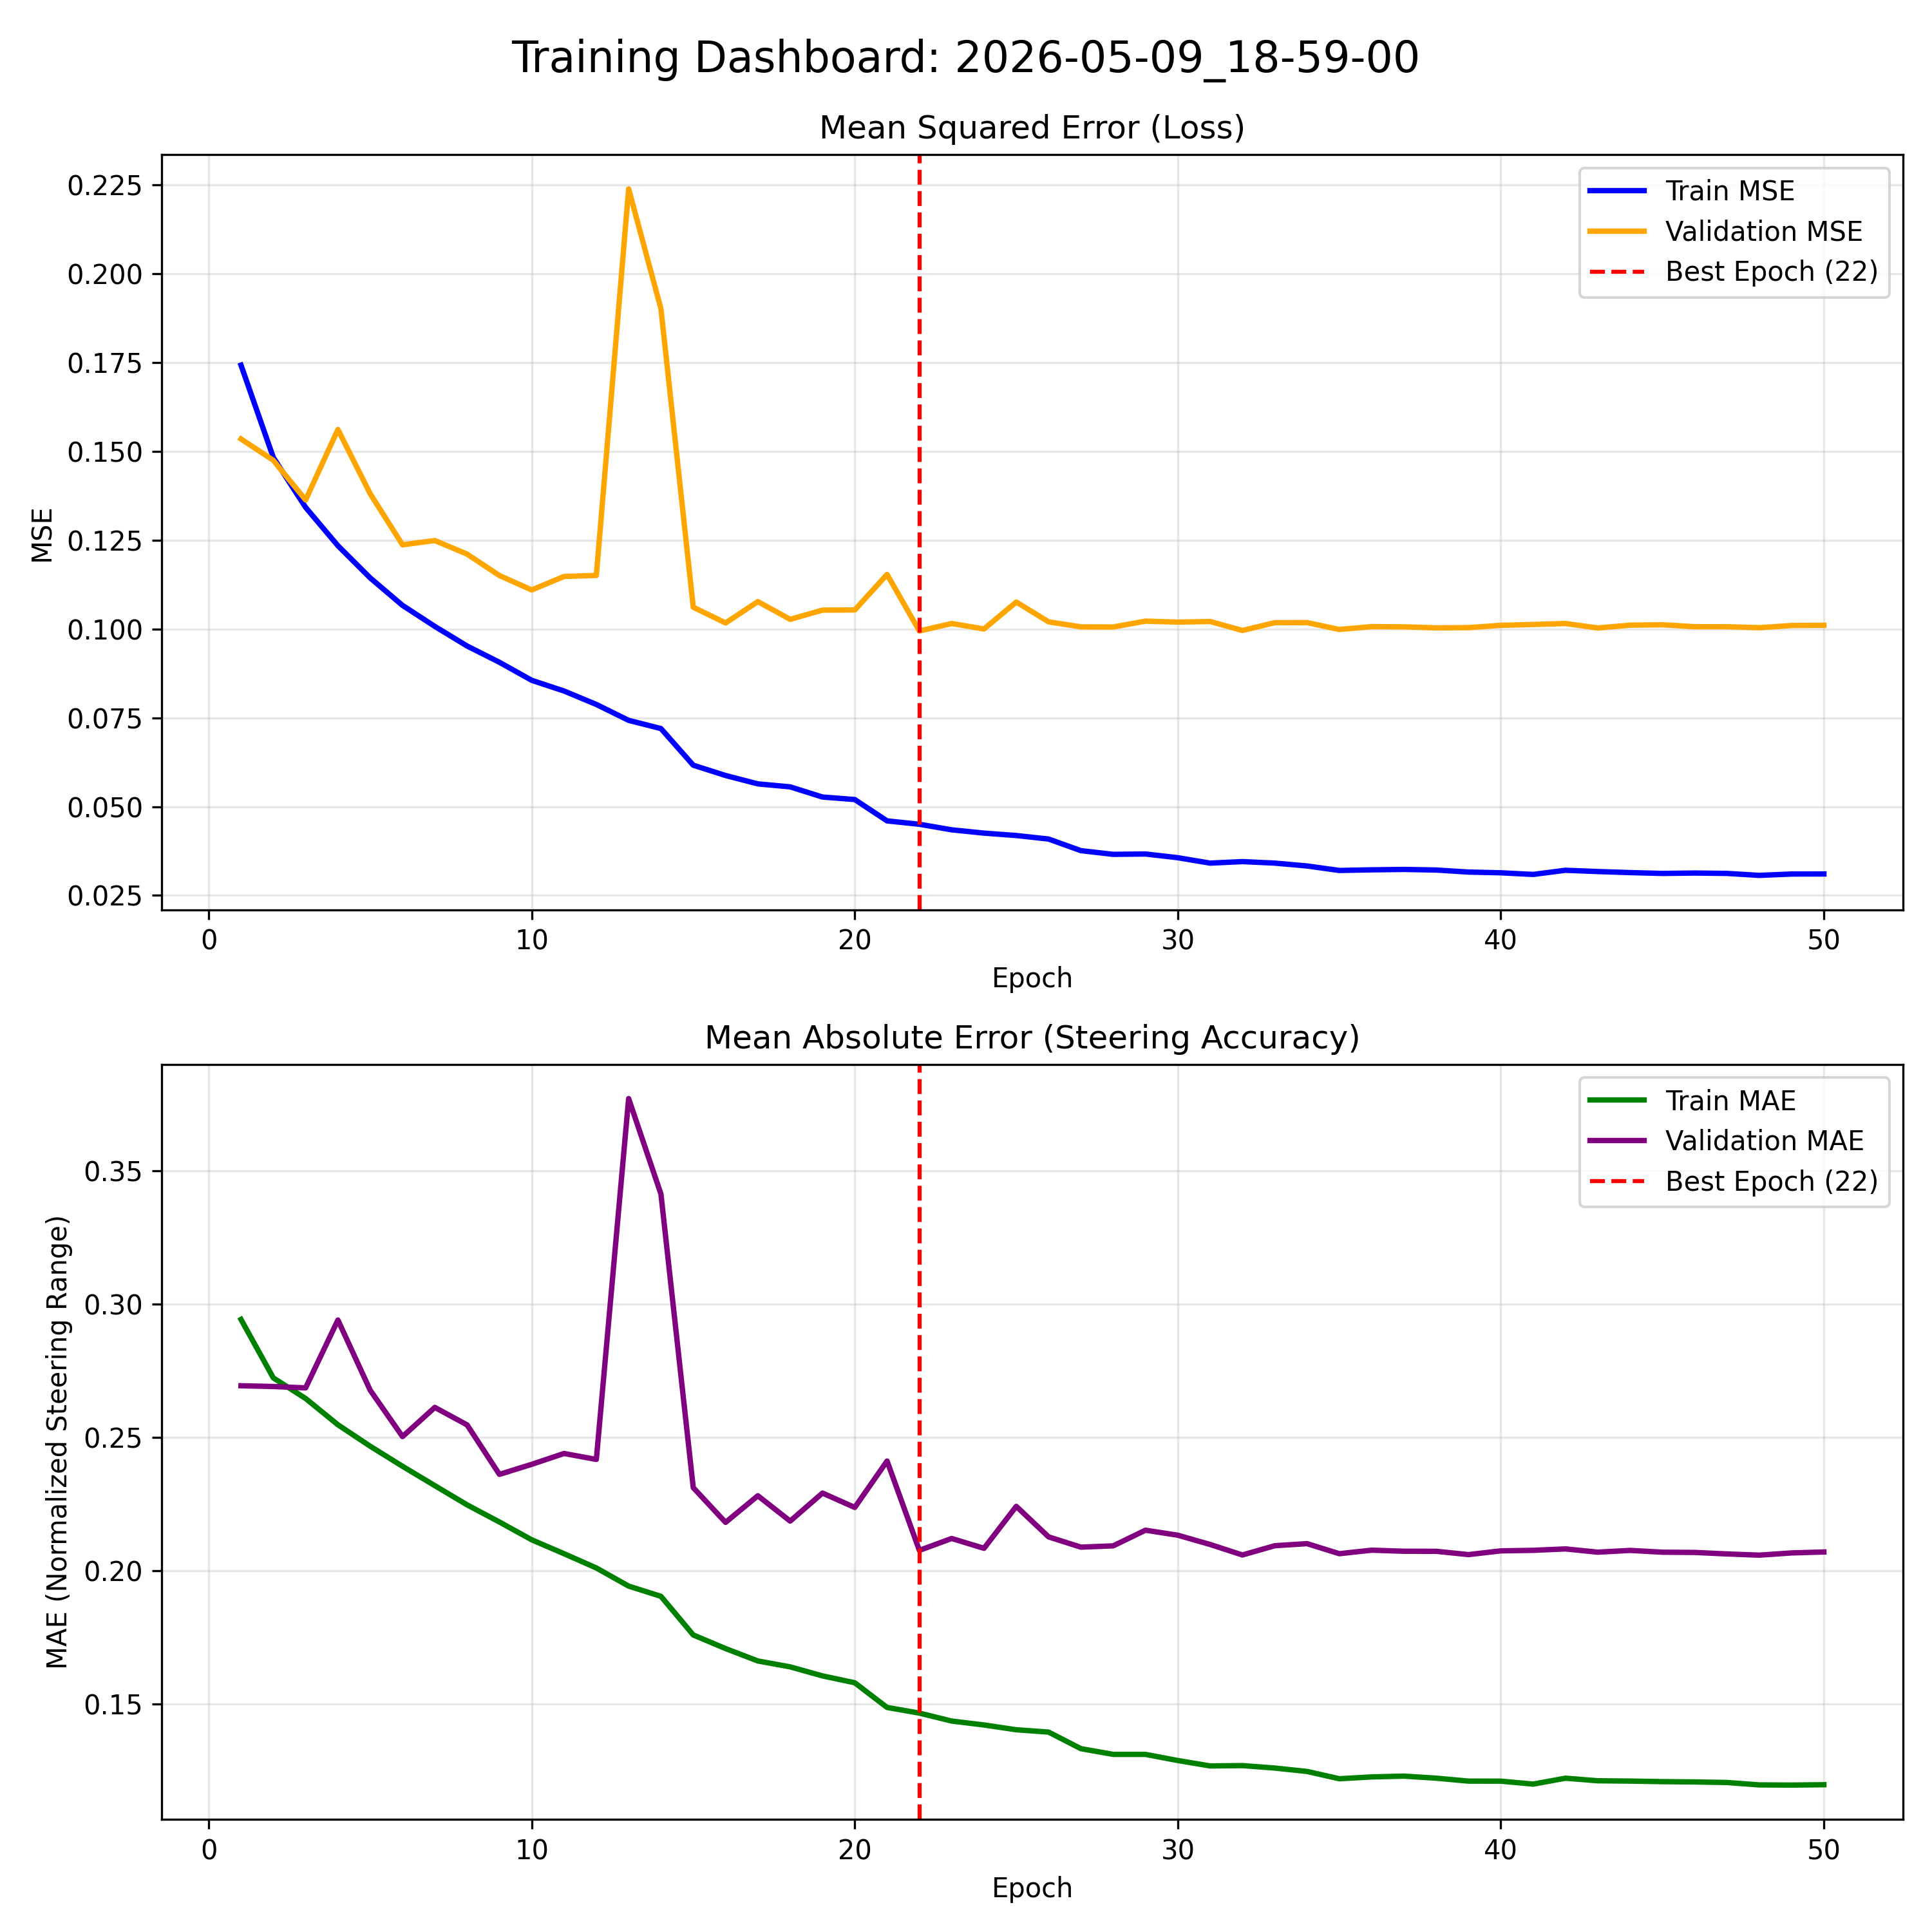
\includegraphics[width=1.0\linewidth]{chap4/images/4th-session.png}
	\caption{The Feature-Extracted Allocentric Model's training profile was unstable, with severe validation noise and a massive loss spike, indicating the network struggled without background shortcuts.}\label{fig:4.3}
\end{figure}

Limited real-world trials at reduced speed still exposed the same instability. The failure was reproduced across two separate deployment sessions, in which the controller survived only 772 and 1{,}122 frames with CTE RMSE values of 35.72~px and 84.38~px respectively (Table~\ref{tab:4.1}), confirming that the instability was systematic rather than an isolated event. As shown in Figure~\ref{fig:4.4} for the longer session, the Cross-Track Error (CTE) drifted steadily upward to roughly 80 pixels before collapsing, while the Heading Error hovered around $-20^\circ$ and then jumped abruptly to approximately $+60^\circ$ near the failure point. The steering signal oscillated with a near-zero mean while speed was increased, indicating the controller was reacting to noise rather than tracking a stable path.

\begin{figure}[H]
	\centering
	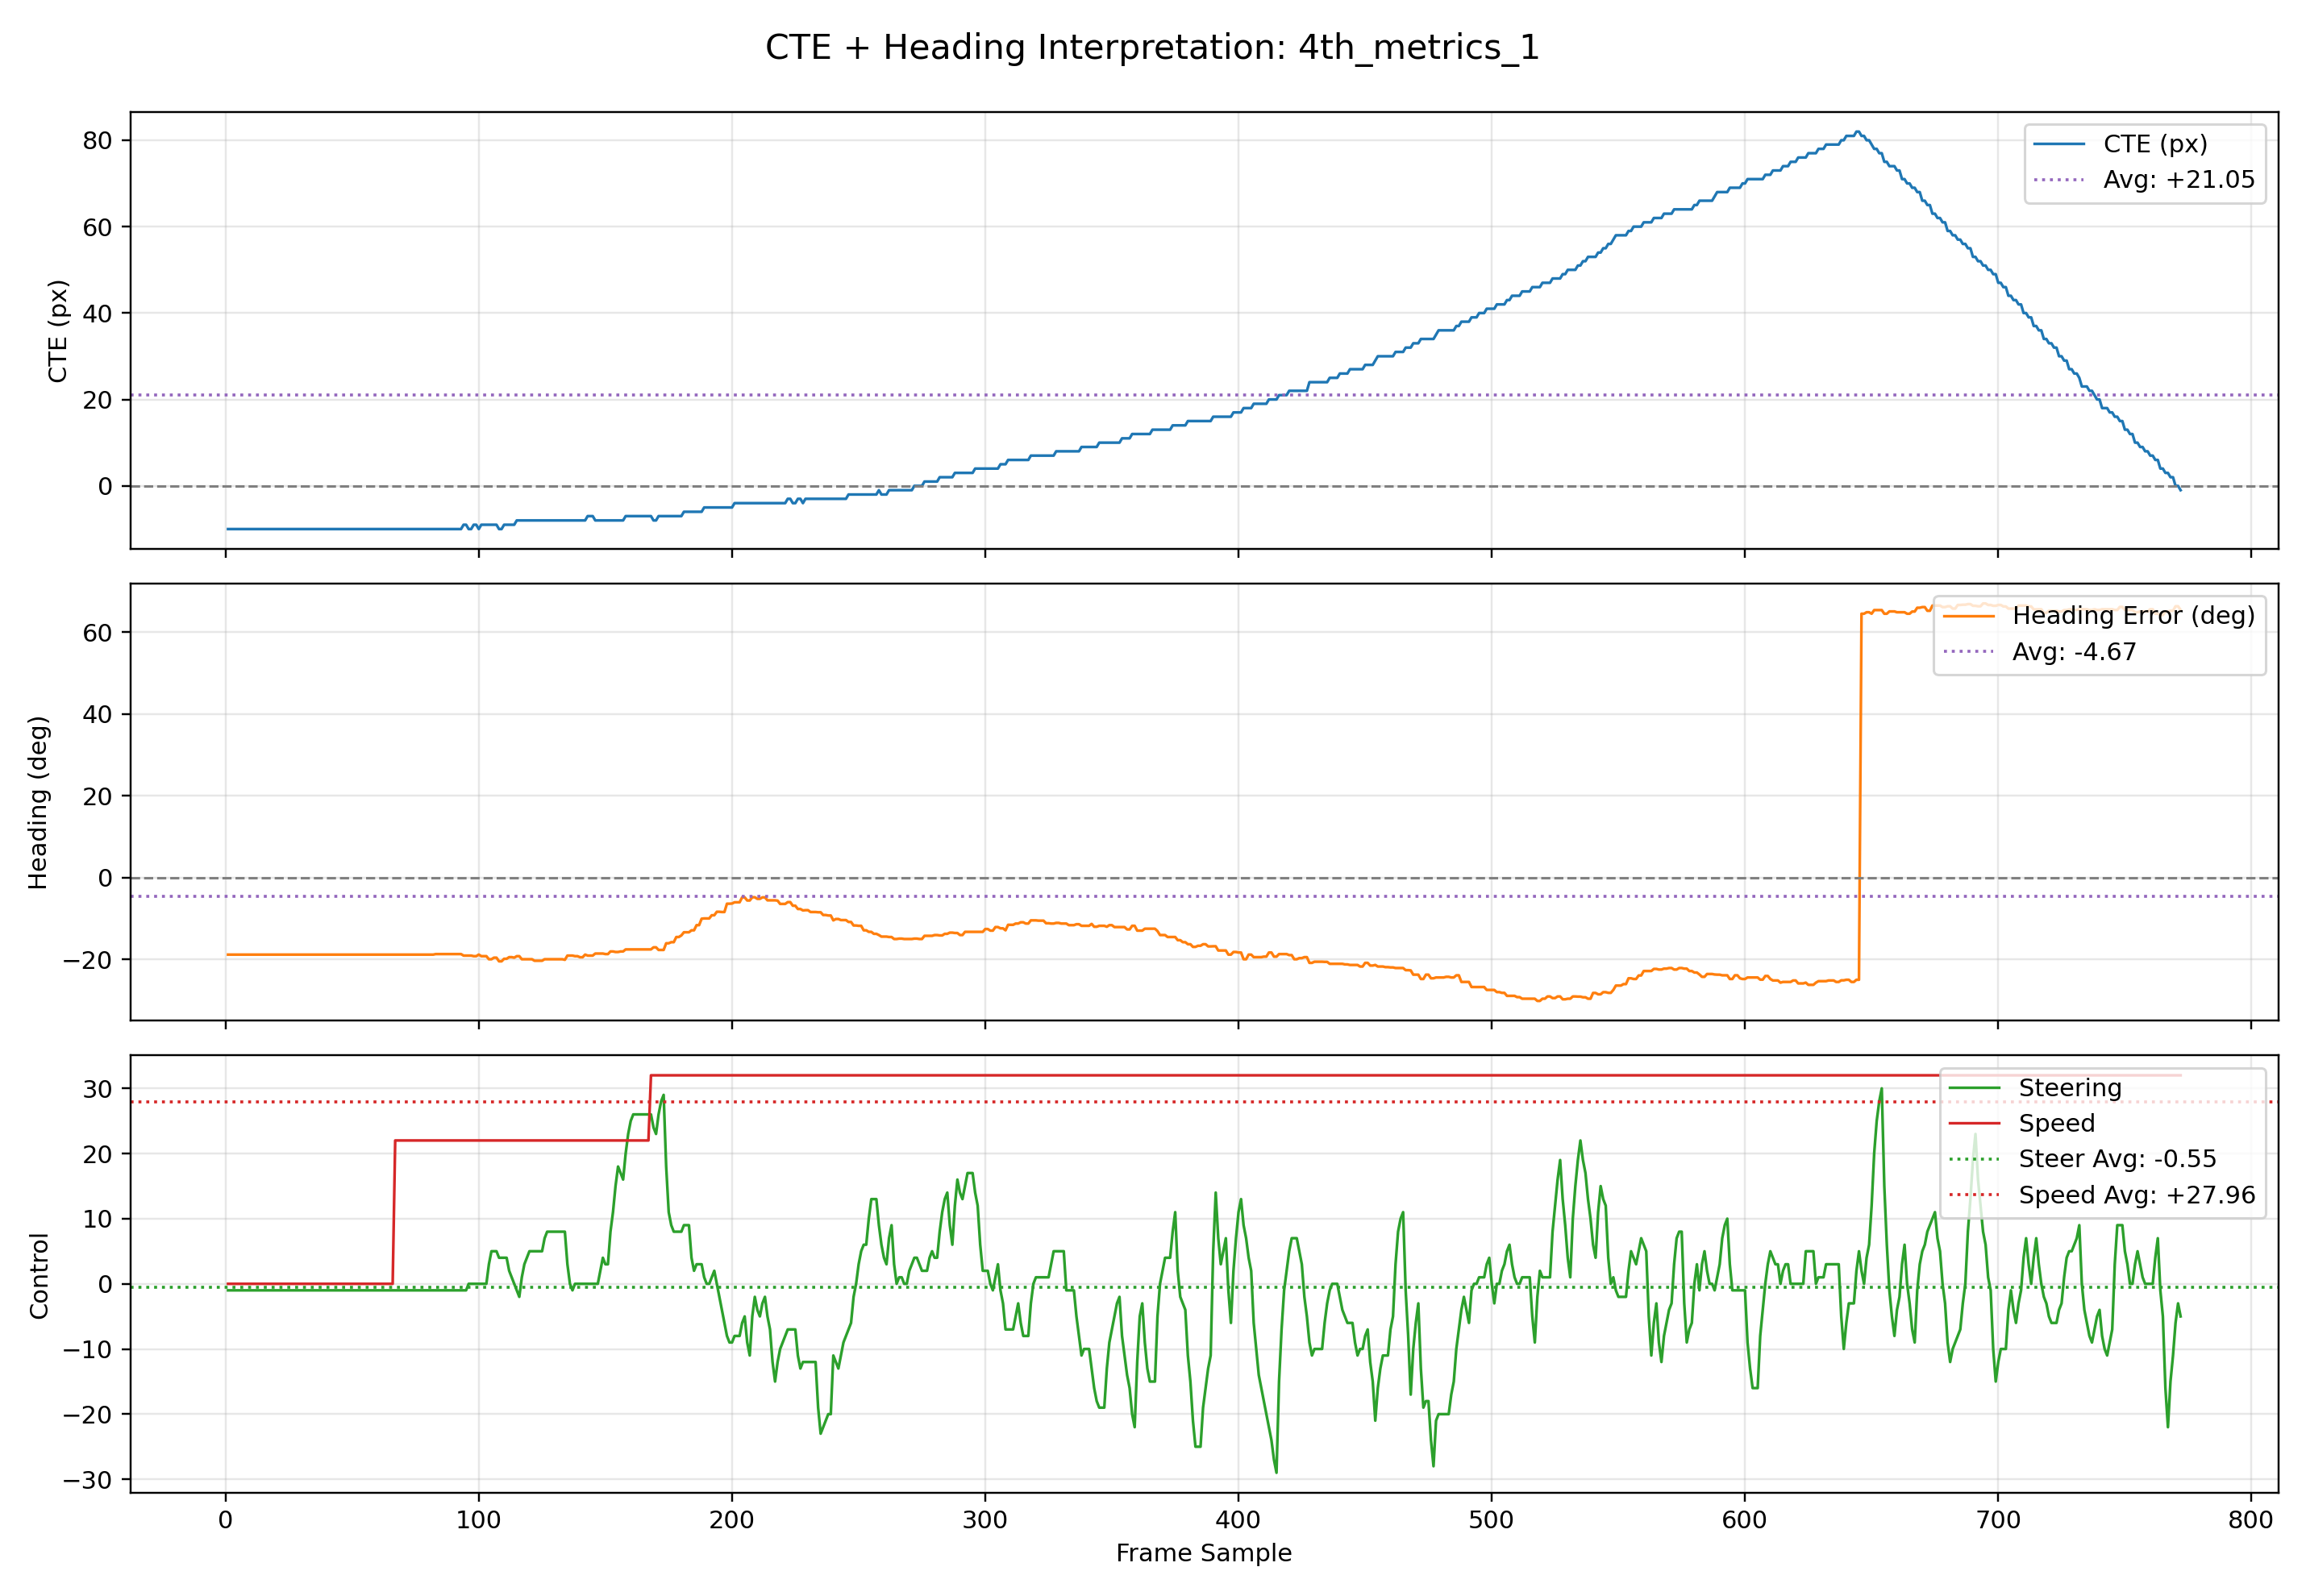
\includegraphics[width=1.0\linewidth]{chap4/images/4th_metrics_1_interpretation.png}
	\caption{Limited real-world trial for Baseline B. CTE drifted upward with a late-stage heading discontinuity, while steering oscillations persisted under increasing speed.}\label{fig:4.4}
\end{figure}

\subsection*{Failure Analysis of Baselines A and B}
The two allocentric baselines failed for complementary reasons that both trace back to the state representation. Baseline A preserved the full room context, which enabled shortcut learning: the CNN exploited static background cues and absolute pixel coordinates rather than learning the path geometry. This produced excellent offline metrics but catastrophic real-world generalization under even minor pose shifts.

Baseline B removed the environmental shortcuts, but the allocentric frame still did not encode the robot's egocentric heading and local path curvature in a stable way. The mapping from a global, top-down AOI to a precise steering command became ambiguous and noise-sensitive, leading to unstable training dynamics and a controller that could not be stabilized for deployment.

Together, these failures established the need for a representation that is both egocentric and dynamically aligned to the robot's local path context, motivating the subsequent Egocentric Dynamic Crop Model.

\section{The Egocentric Dynamic Crop Model}
To resolve both the shortcut learning of Iteration 1 and the spatial translation issues of Iteration 2, the final proposed model implemented the Egocentric Dynamic Crop.

By cropping the image continuously around the ArUco marker, the robot's position remains fixed at the center of the neural network's view. With the background removed, the path geometry simply rotates and approaches the robot, forcing the CNN to learn actual driving rules based strictly on path curvature.
\subsection{Offline Training Convergence}
The proposed model resolved the previous instability issues. By centering the image on the robot, the network required only 9,679 samples to establish geometric stability.

\begin{figure}[H]
	\centering
	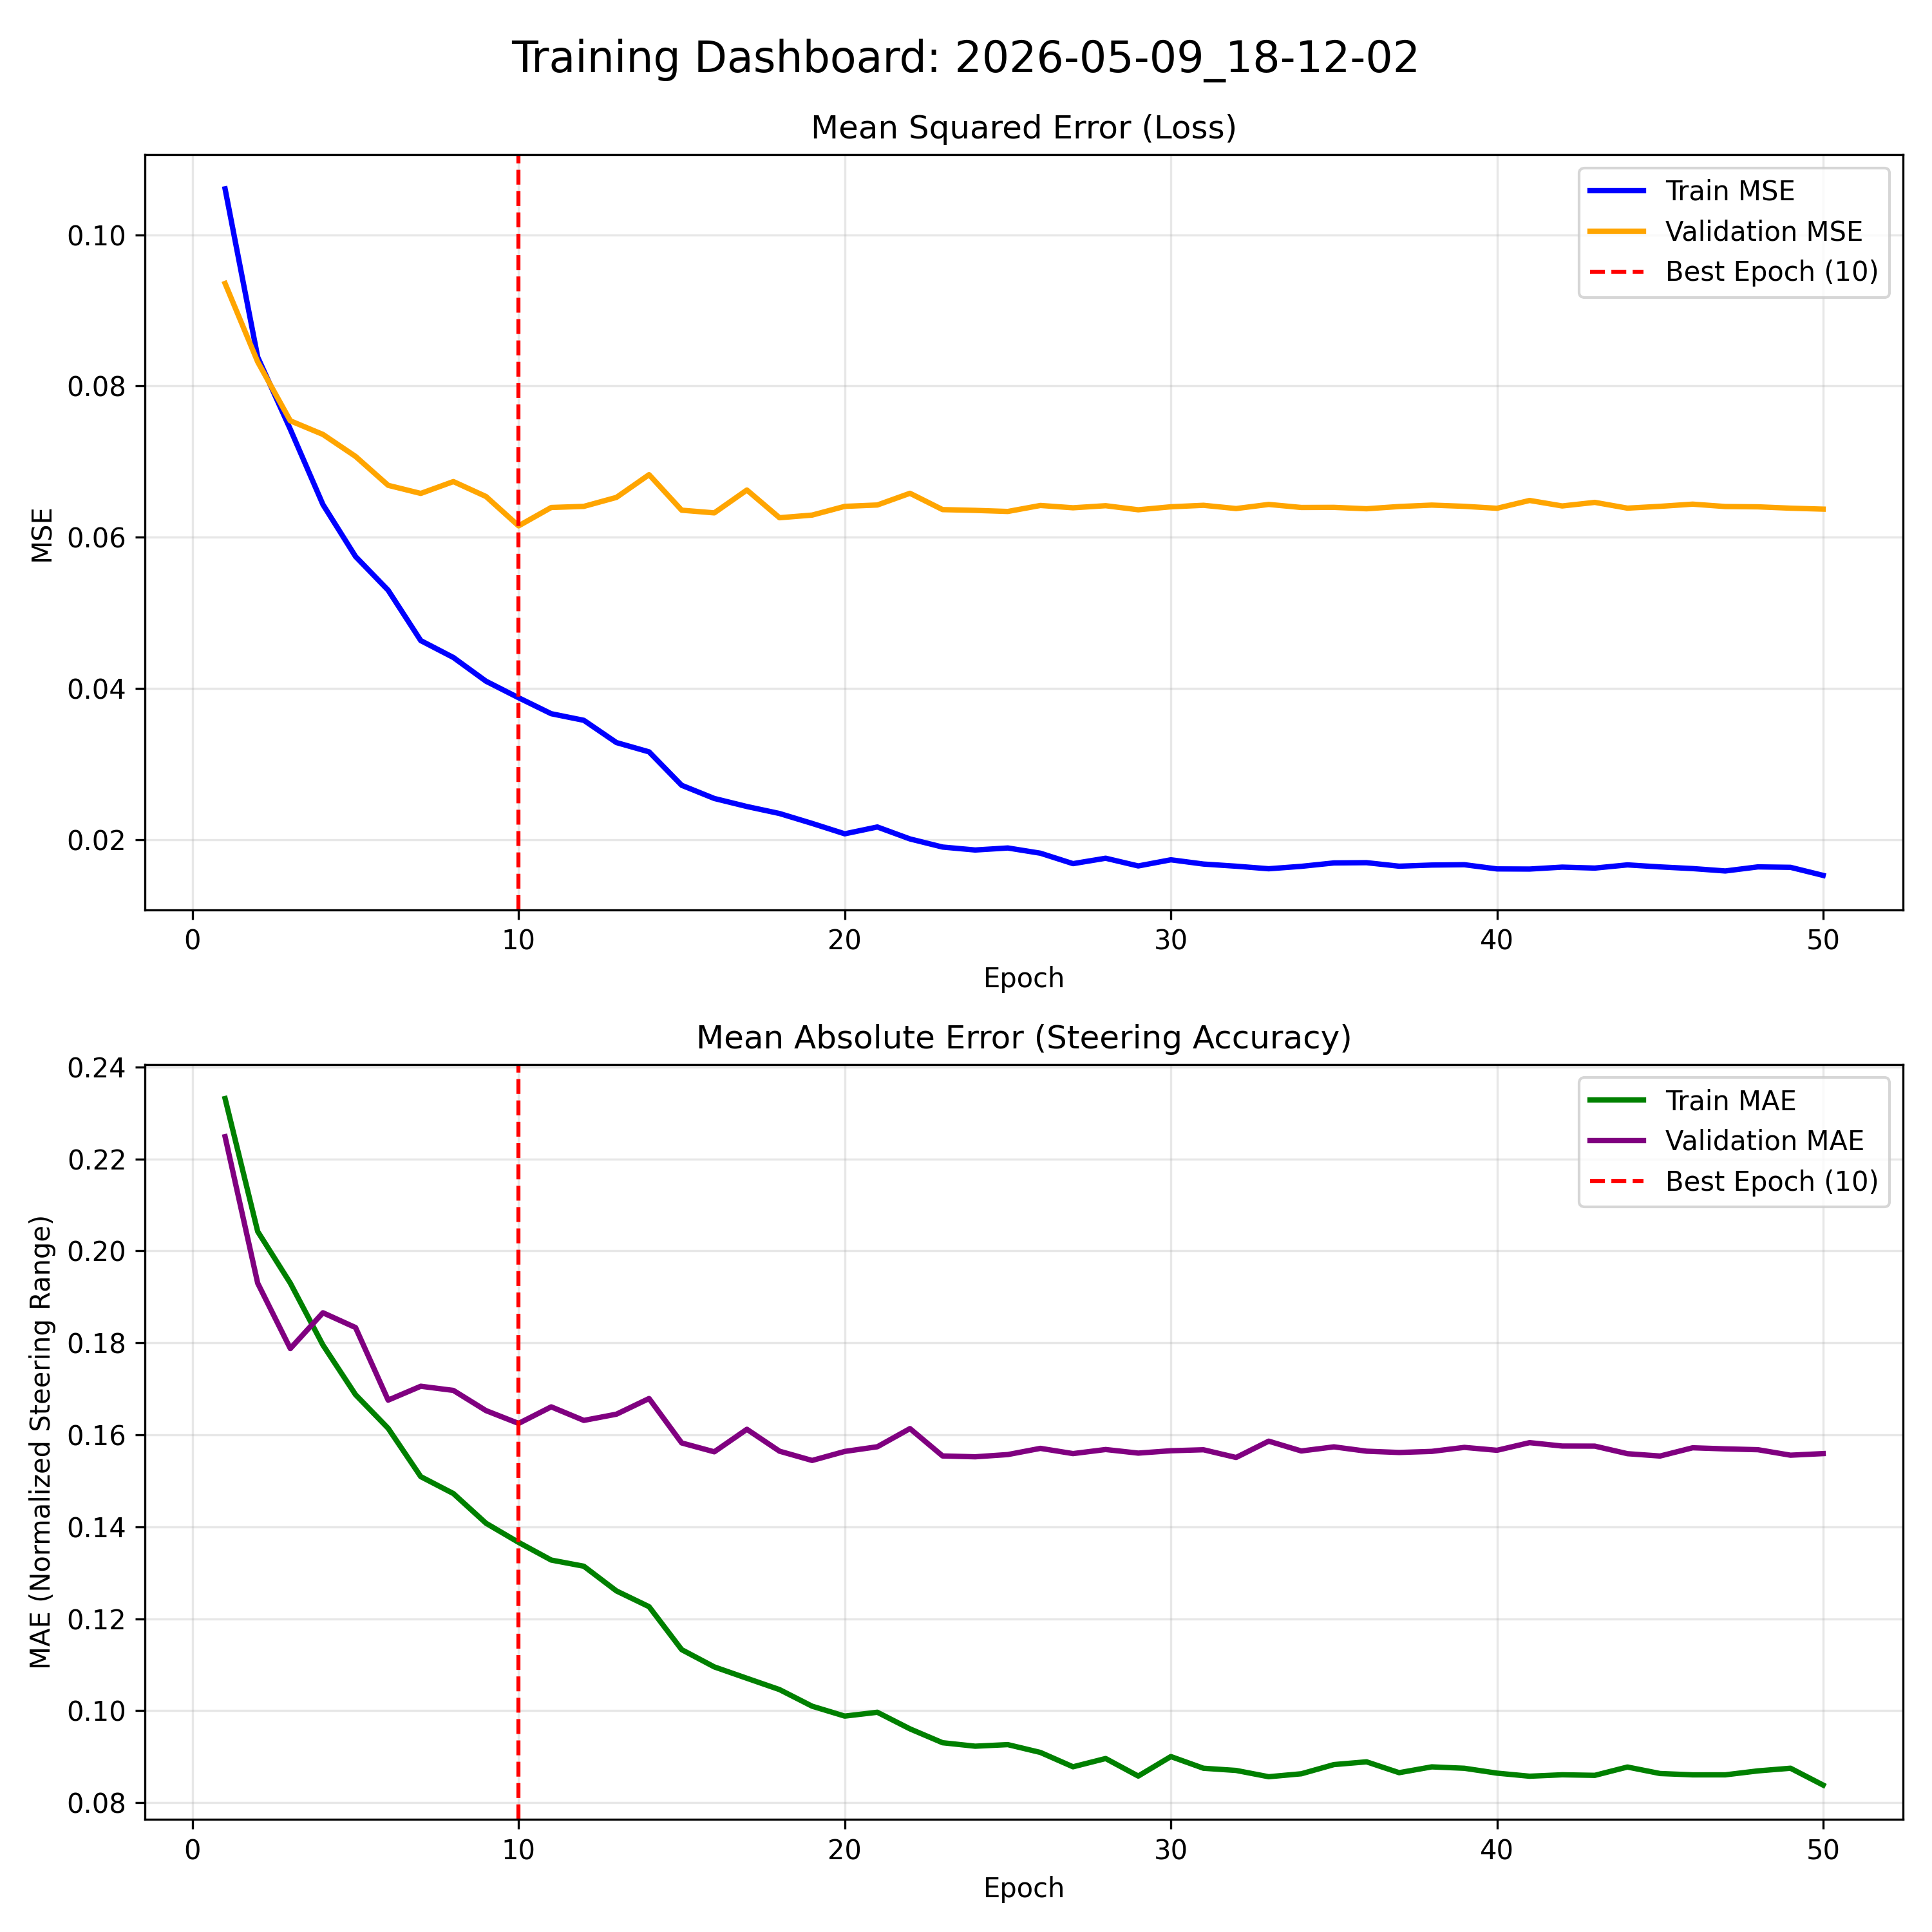
\includegraphics[width=1.0\linewidth]{chap4/images/best_model_metrics.png}
	\caption{The Egocentric Dynamic Crop Model's training profile showed stable convergence, with both MSE and MAE decreasing steadily without significant validation noise.}\label{fig:4.5}
\end{figure}

As shown in Figure~\ref{fig:4.5}, it quickly achieved a highly stable validation MSE of 0.0615 by Epoch 10. The entire optimization process was completed in just 2 minutes and 24 seconds, proving the model is both accurate and computationally lightweight.

\subsection{Real-World Navigation and Endurance}

The proposed Egocentric Model successfully guided the robot through the entire track.

\begin{figure}[H]
	\centering
	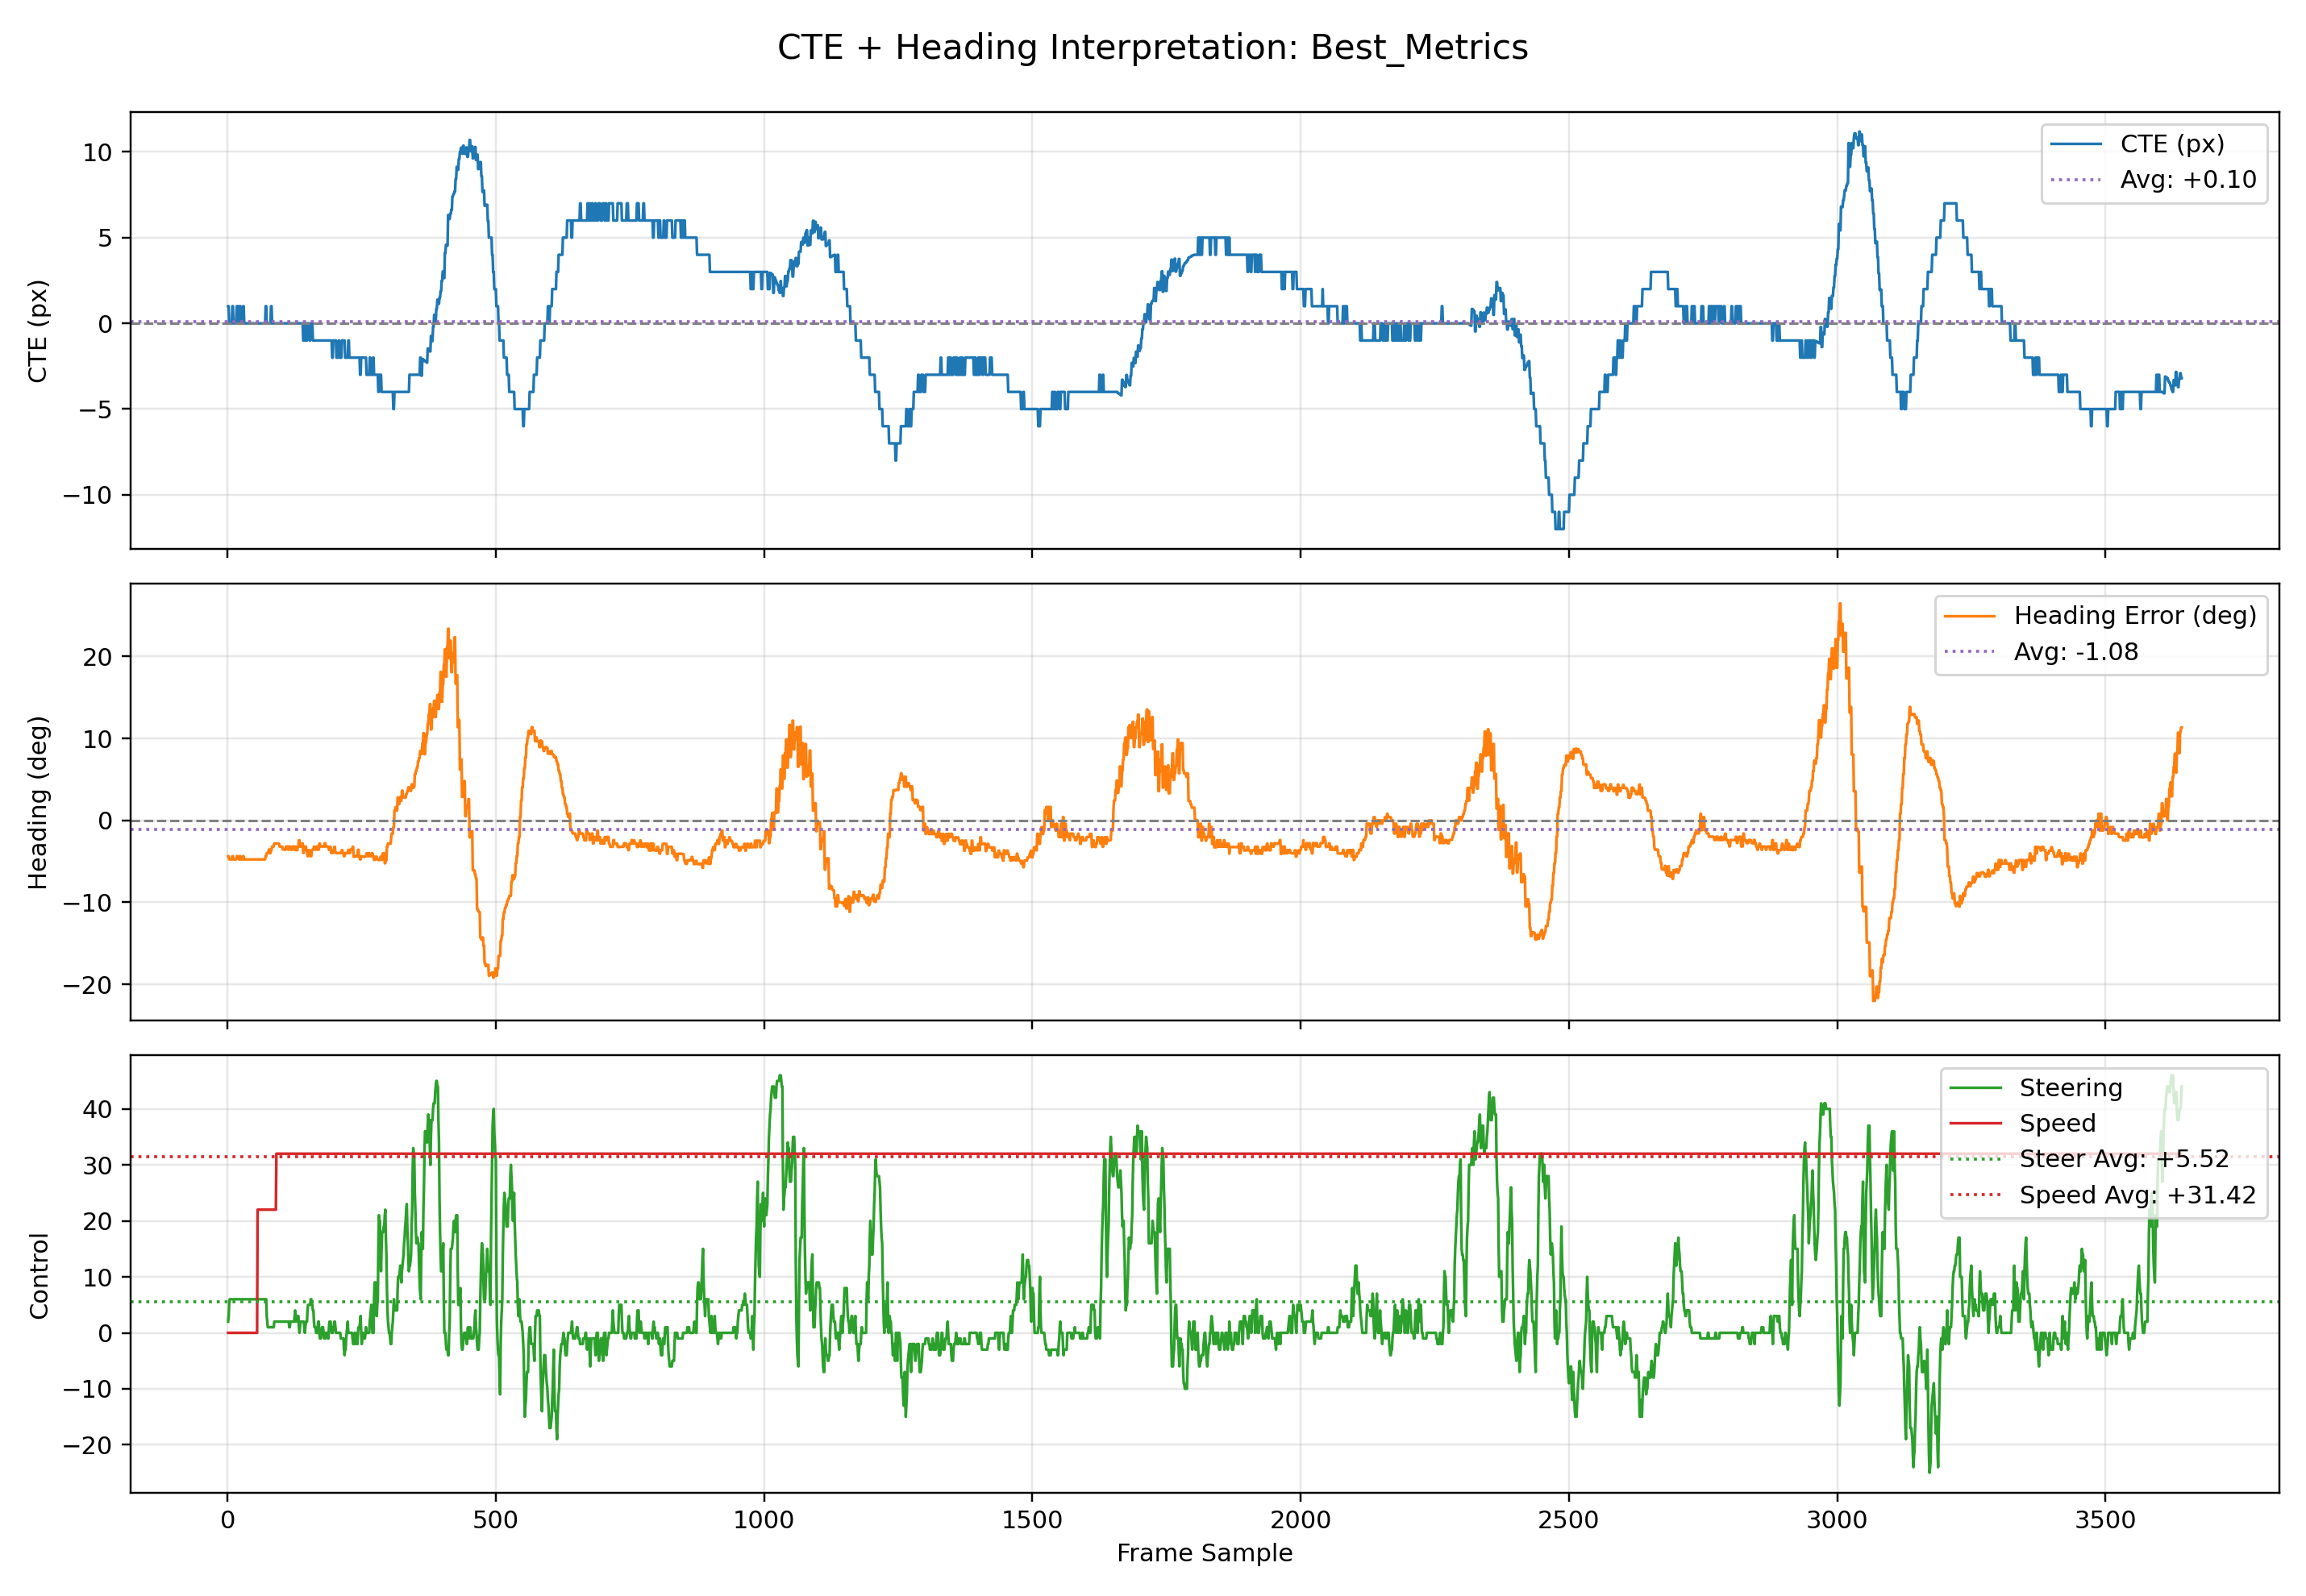
\includegraphics[width=1.0\linewidth]{chap4/images/Best_Metrics_interpretation.png}
	\caption{Physical deployment of the Egocentric Dynamic Crop Model resulted in successful navigation through the entire track, with stable CTE and Heading Error profiles.}\label{fig:4.6}
\end{figure}

Deployed over a continuous run of 3,642 frames, it achieved an extremely low tracking error with an RMSE of 4.0249 pixels and a Mean Absolute CTE of just 3.1700 pixels. The telemetry in Figure 4.6 demonstrates smooth, consistent steering across both straightaways and sharp turns without a single boundary breach.

\section{Comparative Tracking Performance}
Table~\ref{tab:4.1} and Figure~\ref{fig:4.7} summarize the final real-world tracking metrics across all three chronological iterations, clearly illustrating the dramatic stability improvements achieved by the egocentric crop.

\begin{table}[H]
\centering
\caption{Physical Track Testing Results Across All Iterations}
\label{tab:4.1}
\begin{tabularx}{\linewidth}{l X r X r}
\toprule
\textbf{Physical Trial} & \textbf{Active Model} & \textbf{Total Frames Survived} & \textbf{Track Outcome} & \textbf{CTE (RMSE, px)} \\
\midrule
Baseline A & Baseline A (Full AOI) & 636 & Drove off track & 30.9992 \\
Baseline B (Session 1) & Baseline B (Feature-Extracted) & 772 & Drove off track & 35.7224 \\
Baseline B (Session 2) & Baseline B (Feature-Extracted) & 1,122 & Drove off track & 84.3785 \\
Final System & Proposed Egocentric Model & 3,642 & Completed successfully & 4.0249 \\
\bottomrule
\end{tabularx}
\end{table}

\begin{figure}[H]
	\centering
	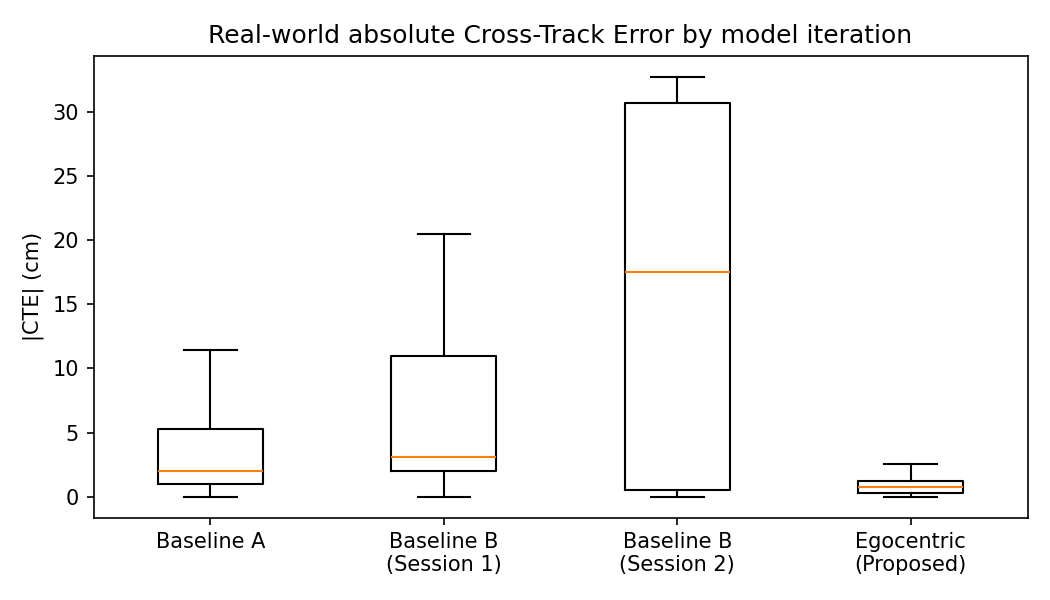
\includegraphics[width=1.0\linewidth]{chap4/images/absolute_cte_boxplot.png}
	\caption{Real-World Trajectory Deviations: Absolute Cross-Track Error Box Plot.}\label{fig:4.7}
\end{figure}
The box plot in Figure~\ref{fig:4.7} shows a dramatic contraction of the error distribution for the proposed model, with a much lower median and tighter interquartile range than Baselines A and B. This indicates not only lower average tracking error but also substantially reduced variability and fewer large deviations.

\section{In-Depth Performance of the Model}
To comprehensively validate the proposed end-to-end architecture, the Egocentric Dynamic Crop model was evaluated across three specific track topologies of increasing B{\'e}zier curve complexity. By entirely removing the PID control components and relying strictly on the Convolutional Neural Network (CNN) for high-level navigation, this phase of testing isolates the controller's ability to dynamically scale continuous steering outputs based solely on visual geometric features.

\subsection{Statistical Analysis Methodology}
For each evaluation scenario, the robot was deployed in a continuous autonomous run during which the tracking system recorded per-frame Cross-Track Error (CTE) and Heading Error at approximately 60~Hz. To evaluate tracking consistency over sustained periods, telemetry is resolved per \emph{lap} rather than over arbitrary fixed-length frame windows. A lap represents one complete physical circuit of the track, aligning each consistency window with a meaningful unit of the course rather than a time-slice that spans variable parts of a circuit. Laps are partitioned by dividing the total duration of each scenario by the number of complete laps. Mirroring the policy of excluding incomplete segments, partial trailing laps (e.g., the final 14.3~s of the Scenario 3 run) are discarded so that only complete circuits contribute. The full quantitative summary is presented in Tables~\ref{tab:4.2}, \ref{tab:per_lap_consistency}, and \ref{tab:per_lap_detail}.

All cross-track errors are measured in the rectified bird's-eye-view canvas, which spans $800 \times 800$~pixels and maps to the physical arena of approximately $2.0$--$3.0$~m per side. Adopting a nominal arena width of $2.5$~m yields a scale of approximately $0.31$~cm per pixel, which is used throughout this chapter to report approximate real-world deviations alongside the pixel measurements. Because the physical arena dimension is approximate, the centimetre figures are likewise approximate (to within roughly $\pm 20\%$). The steering command reported throughout is the raw controller command after scaling the network's normalized output (scaling gain $k_{steer}=50$, clipped to $[-50,50]$), where positive values denote rightward turns and negative values leftward turns. Commands between $-2$ and $2$ are treated as straight-line driving (deadband). Empirically, this raw command maps monotonically to the robot's measured yaw rate and saturates at high-magnitude commands as the differential-drive platform reaches its motor limits; the values are therefore reported as unitless command magnitudes rather than physical angles.

\begin{table}[H]
\centering
\caption{Kinematic Performance Summary of the Final Egocentric Model}
\label{tab:4.2}
\footnotesize
\begin{tabularx}{\linewidth}{@{}l X r r r r@{}}
\toprule
 & & & \multicolumn{3}{c@{}}{\textbf{Cross-Track Error (px)}} \\
\cmidrule(l){4-6}
\textbf{Scenario} & \textbf{Track Topology} & \textbf{Frames} & \textbf{Mean $\pm$ SD} & \textbf{RMSE} & \textbf{P95} \\
\midrule
1 & 45$^\circ$ B{\'e}zier curves & 2{,}934 & 1.91 $\pm$ 1.84 & 2.66 & 5.0 \\
2 & 90$^\circ$ square path & 1{,}709 & 2.74 $\pm$ 2.23 & 3.54 & 8.0 \\
3 & 180$^\circ$ sustained U-turn & 13{,}421 & 5.07 $\pm$ 4.62 & 6.86 & 15.0 \\
\bottomrule
\end{tabularx}
\end{table}

% chap4/per_lap_consistency.tex
% Trial-to-trial CTE RMSE consistency over N=10 independent randomized-start trials per scenario.
% Replaces the old per-lap (within-one-run) analysis. \input this into Chapter 4.

\subsection{Trial-to-Trial Tracking Consistency}
\label{sec:per_lap_consistency}
Because each evaluation trial is exactly one circuit of the track, the repeated unit is the
\emph{independent trial} rather than a lap within a continuous run. Tracking consistency is therefore
reported as the distribution of per-trial CTE RMSE across the $N=10$ randomized-start trials of each
scenario (Table~\ref{tab:per_lap_consistency}).

\begin{table}[H]
\centering
\caption{Trial-to-trial CTE RMSE consistency ($N=10$ independent randomized-start trials per scenario).}
\label{tab:per_lap_consistency}
\footnotesize
\begin{tabular}{@{}l r r r@{}}
\toprule
\textbf{Scenario} & \textbf{Trials ($n$)} & \textbf{Per-trial RMSE mean $\pm$ SD (cm)} & \textbf{Range (cm)} \\
\midrule
1 (45$^\circ$)   & 10 & 0.98 $\pm$ 0.11 & 0.76--1.15 \\
2 (90$^\circ$)   & 10 & 1.49 $\pm$ 0.14 & 1.26--1.69 \\
3 (180$^\circ$)  & 10 & 0.91 $\pm$ 0.04 & 0.86--0.96 \\
4 (held-out)     & 10 & 2.04 $\pm$ 0.16 & 1.77--2.44 \\
\bottomrule
\end{tabular}
\end{table}

The small standard deviations (0.04--0.17~cm) are the central result: the controller produces
near-identical tracking error across independent trials that each start from a different randomized
pose, indicating high repeatability rather than a single lucky run. The trained-track scenarios
(1--3) cluster tightly, while the held-out track (Scenario~4) shows both a higher mean and a wider
spread, consistent with the generalization gap reported in Section~\ref{sec:generalization}.


\subsection{Scenario 1: 45-Degree B{\'e}zier Curves}
The first scenario tests mild, continuous curvature over 2{,}934 frames (49.0~s) of continuous autonomous driving. Rather than exhibiting the fishtailing or oscillatory steering behavior commonly observed in pure behavioral cloning models without derivative damping, the model demonstrated highly anticipatory steering. As the $45^\circ$ curves entered the egocentric bounding box, the convolutional feature extractor registered the gradual geometric shift, resulting in a smooth, continuous adjustment of the steering vector. The model achieved a mean absolute CTE of \textbf{1.91 $\pm$ 1.84}~px (RMSE = 2.66~px, $\approx 0.83$~cm), with 95\% of all frames remaining within 5.0~px ($\approx 1.6$~cm) of the reference path. Per-lap consistency analysis across 10 completed laps yielded a mean per-lap RMSE of \textbf{2.28 $\pm$ 1.37}~px (range: 0.93--4.73~px, Table~\ref{tab:per_lap_consistency}), confirming consistent tracking throughout the run. The Heading Error remained bounded, with a mean of $-1.05 \pm 5.13^\circ$ and peaking at \textbf{31.92$^\circ$} at the sharpest point of the transition, proving that the model does not overreact to gentle path deviations and smoothly tracks shallow curves.

\subsection{Scenario 2: 90-Degree B{\'e}zier Corners (Square Path)}
Navigating the square path over 1{,}709 frames (28.5~s) tested the model's response to rapid, orthogonal geometric changes. The model achieved a mean absolute CTE of \textbf{2.74 $\pm$ 2.23}~px (RMSE = 3.54~px, $\approx 1.1$~cm), with 95\% of frames within 8.0~px ($\approx 2.5$~cm) of the reference path. The Heading Error remained bounded, with a mean of $-3.16 \pm 5.74^\circ$ and a peak magnitude of $20.98^\circ$. Approaching a $90^\circ$ corner requires a sharp spike in actuation. Upon entering the apex of the corners, the model successfully executed aggressive, high-magnitude steering commands, reaching a peak raw steering command magnitude of \textbf{33.0}.

\begin{figure}[H]
	\centering
	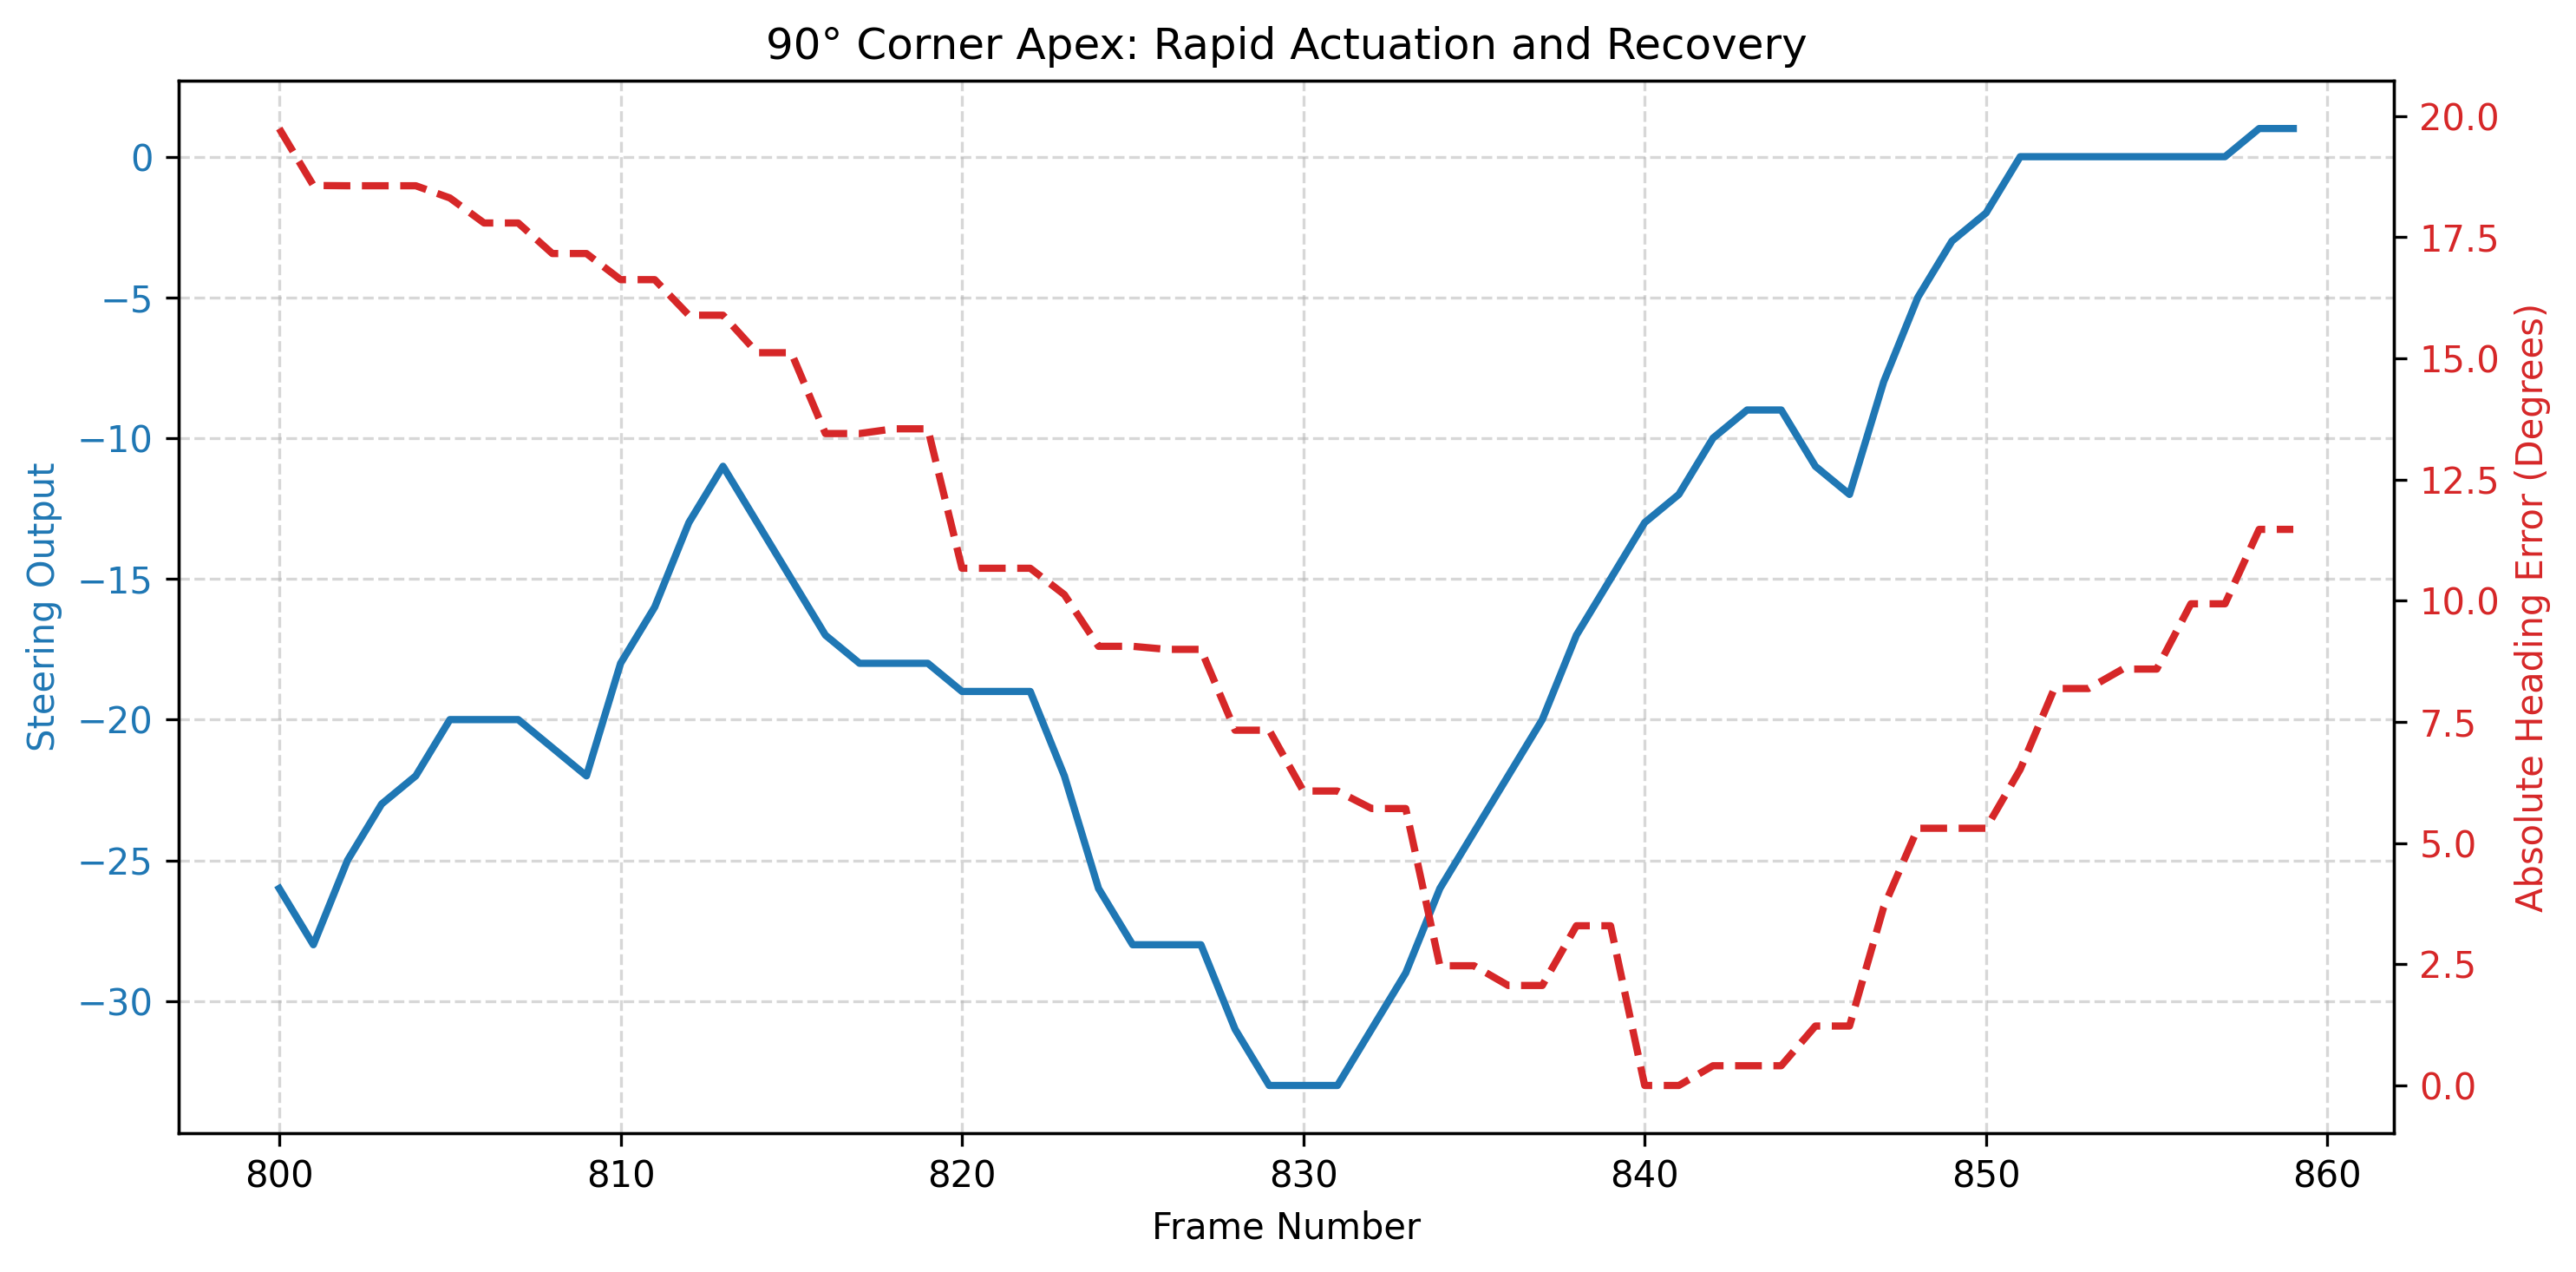
\includegraphics[width=1.0\linewidth]{chap4/images/90_Degree_Telemetry.png}
	\caption{90-degree cornering telemetry showing rapid actuation and recovery under orthogonal curvature.}\label{fig:4.8}
\end{figure}

Importantly, as visualized in Figure~\ref{fig:4.8}, the Egocentric Dynamic Crop ensured that the path boundaries remained centered in the network's view rather than sweeping out of frame. This continuous recentering allowed for a rapid and stable recovery; the model brought the heading error back down to $0^\circ$ within just \textbf{11 frames} (approximately \textbf{0.73 s} at a 15 Hz operating frequency) upon exiting the corner, resuming straight-line stability instantly.

\subsection{Scenario 3: 180-Degree Sustained U-Turns}
The final topology tested the system's kinematic endurance during extreme, continuous curvature. This scenario produced the longest continuous run at 13{,}421 frames over 226.5~s (approximately 3.8 minutes) of uninterrupted autonomous driving, encompassing many complete laps of the U-turn track. During the 180-degree U-turns, the model was forced to hold a near-maximum steering angle for a prolonged period.

\begin{figure}[H]
	\centering
	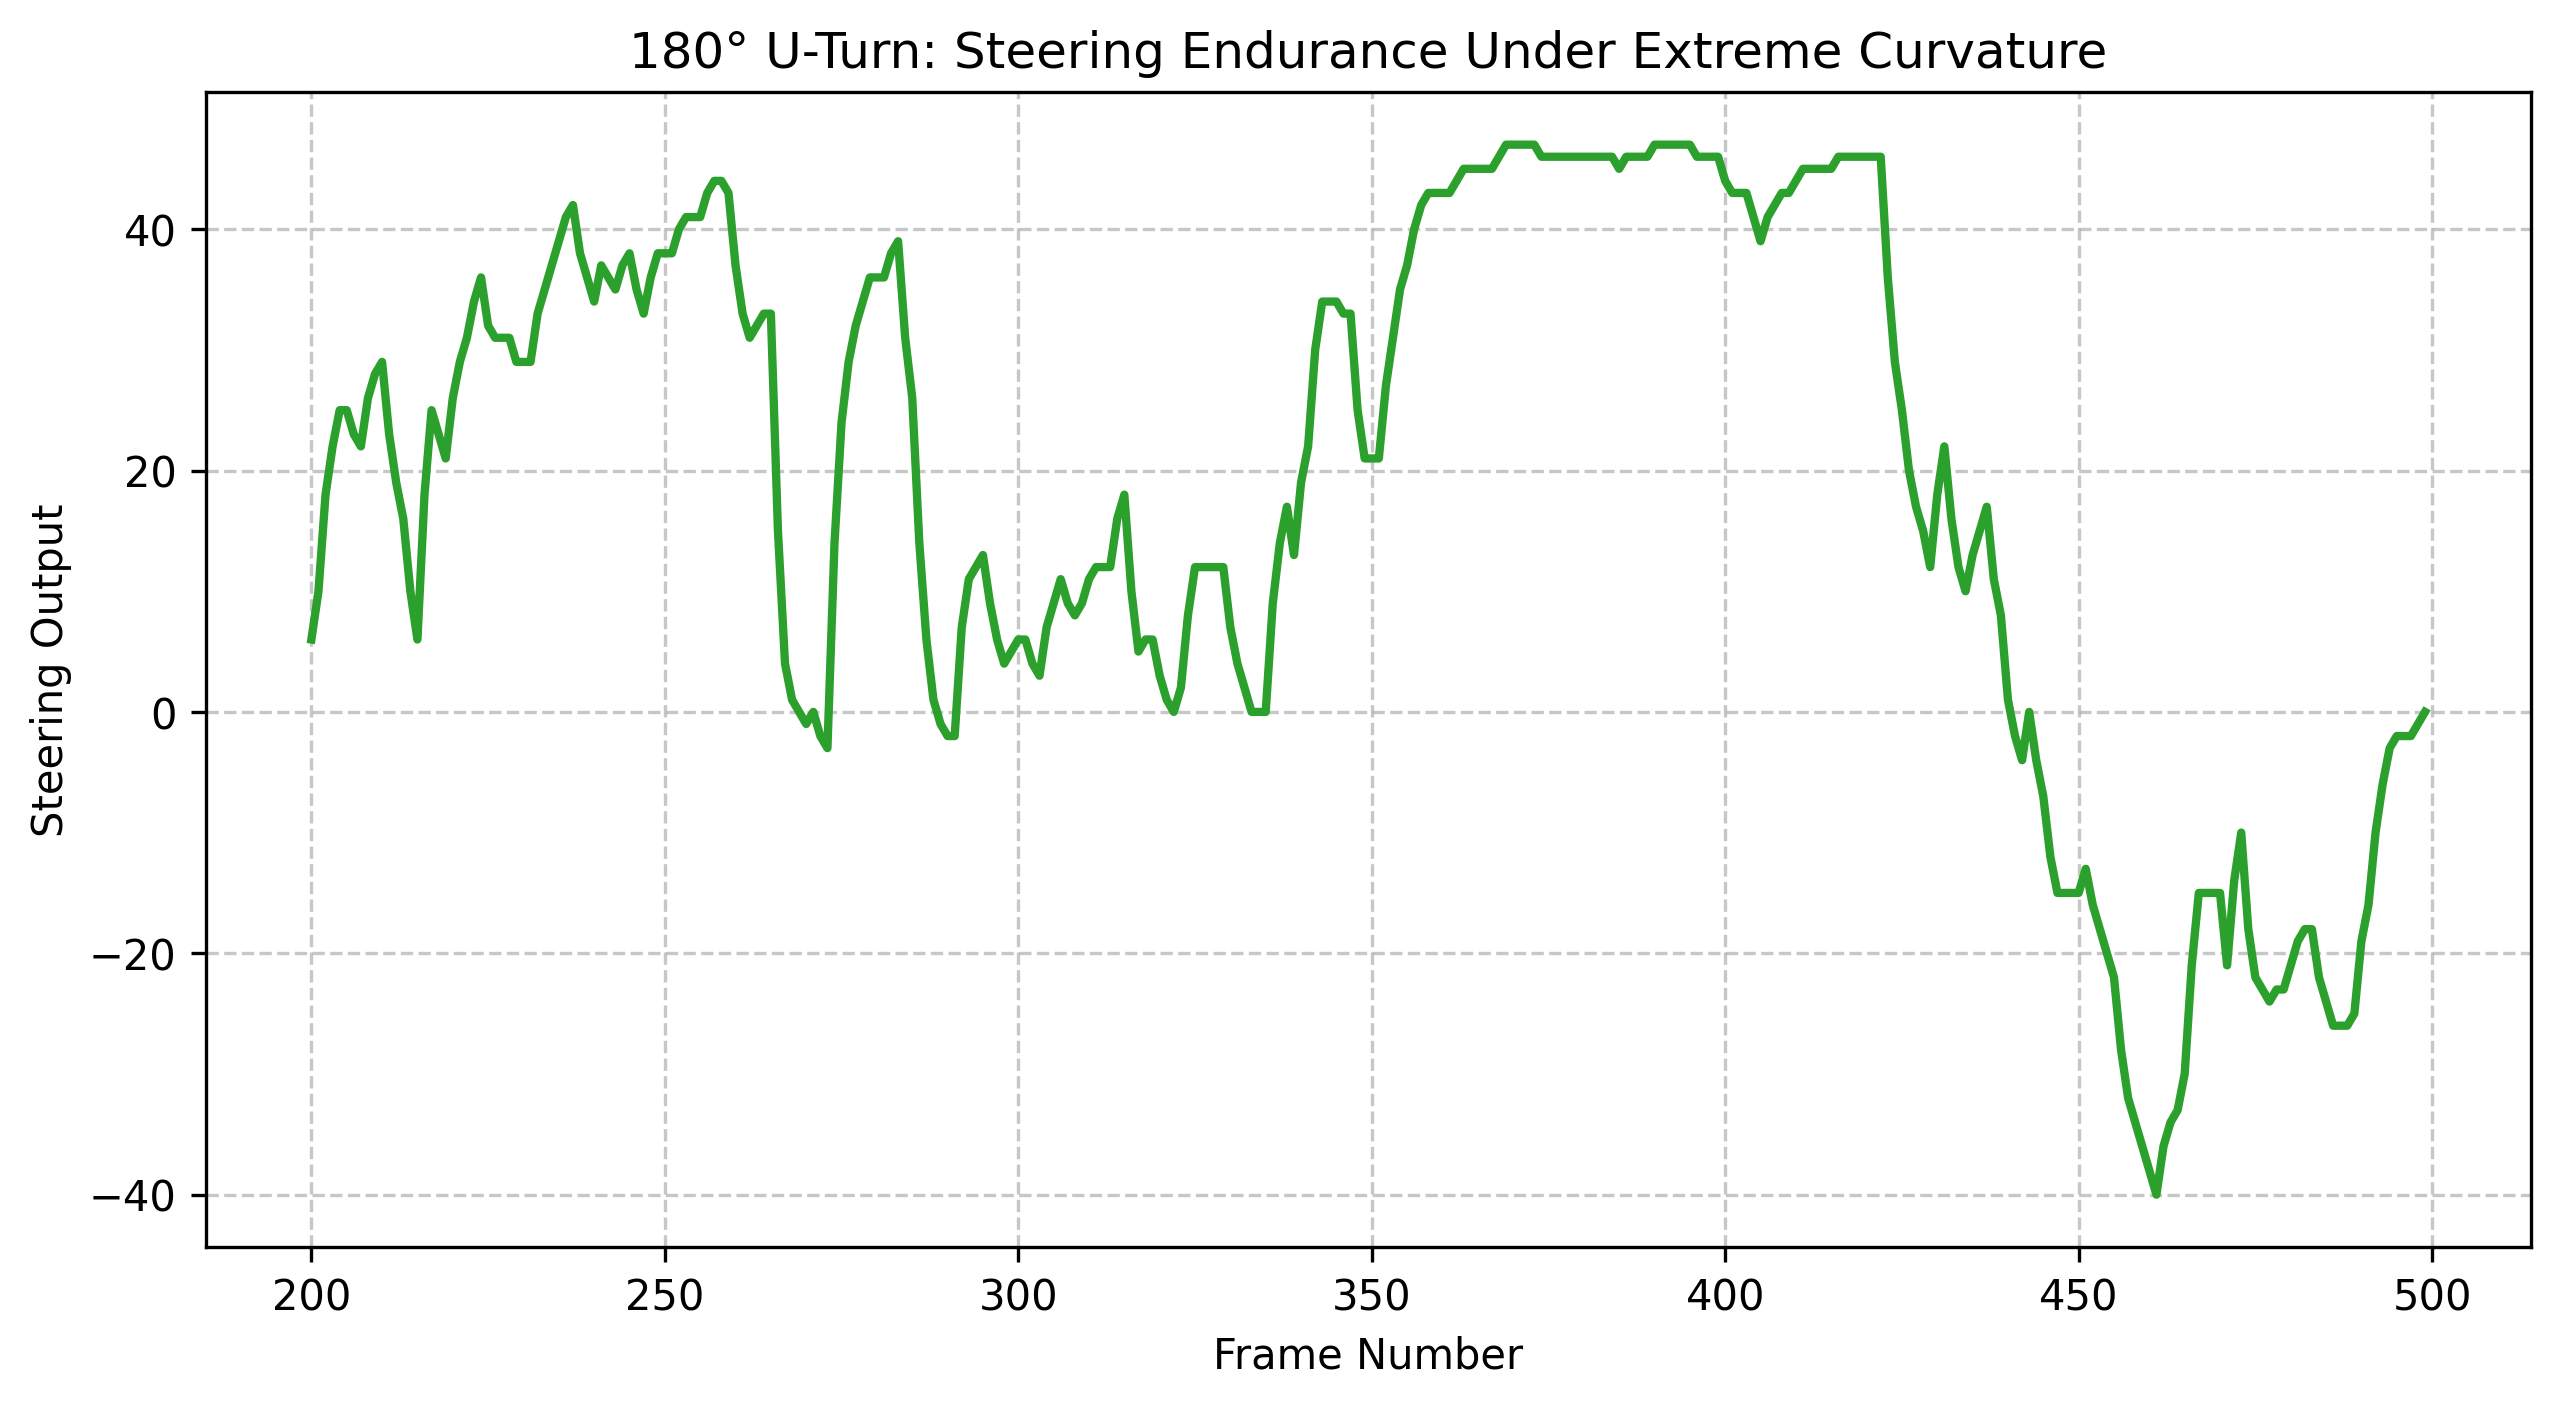
\includegraphics[width=1.0\linewidth]{chap4/images/180_Degree_Endurance.png}
	\caption{180-degree U-turn telemetry illustrating sustained steering actuation under extreme curvature.}\label{fig:4.9}
\end{figure}

The telemetry in Figure~\ref{fig:4.9} confirms that the network successfully handled the extreme geometric distortion, scaling up its actuation to reach and sustain a maximum raw steering command magnitude of \textbf{47.0}. The model achieved a mean absolute CTE of \textbf{5.07 $\pm$ 4.62}~px (RMSE = 6.86~px, $\approx 2.1$~cm), with 95\% of frames within 15.0~px ($\approx 4.7$~cm) of the reference path and a worst-case deviation of 28.9~px ($\approx 9.0$~cm), which remains below half the chassis width. The Heading Error over the run had a mean of $-0.16 \pm 9.34^\circ$ with a peak magnitude of $33.95^\circ$. Per-lap consistency analysis across 8 completed laps yielded a mean per-lap RMSE of \textbf{6.56 $\pm$ 2.08}~px (range: 4.43--10.14~px, Table~\ref{tab:per_lap_consistency}), demonstrating that tracking performance remained bounded throughout the extended run despite the extreme curvature. This confirms that the CNN effectively learned the structural rules of extreme curvature tracking without requiring a rigid mathematical path-planning algorithm.

\begin{figure}[H]
	\centering
	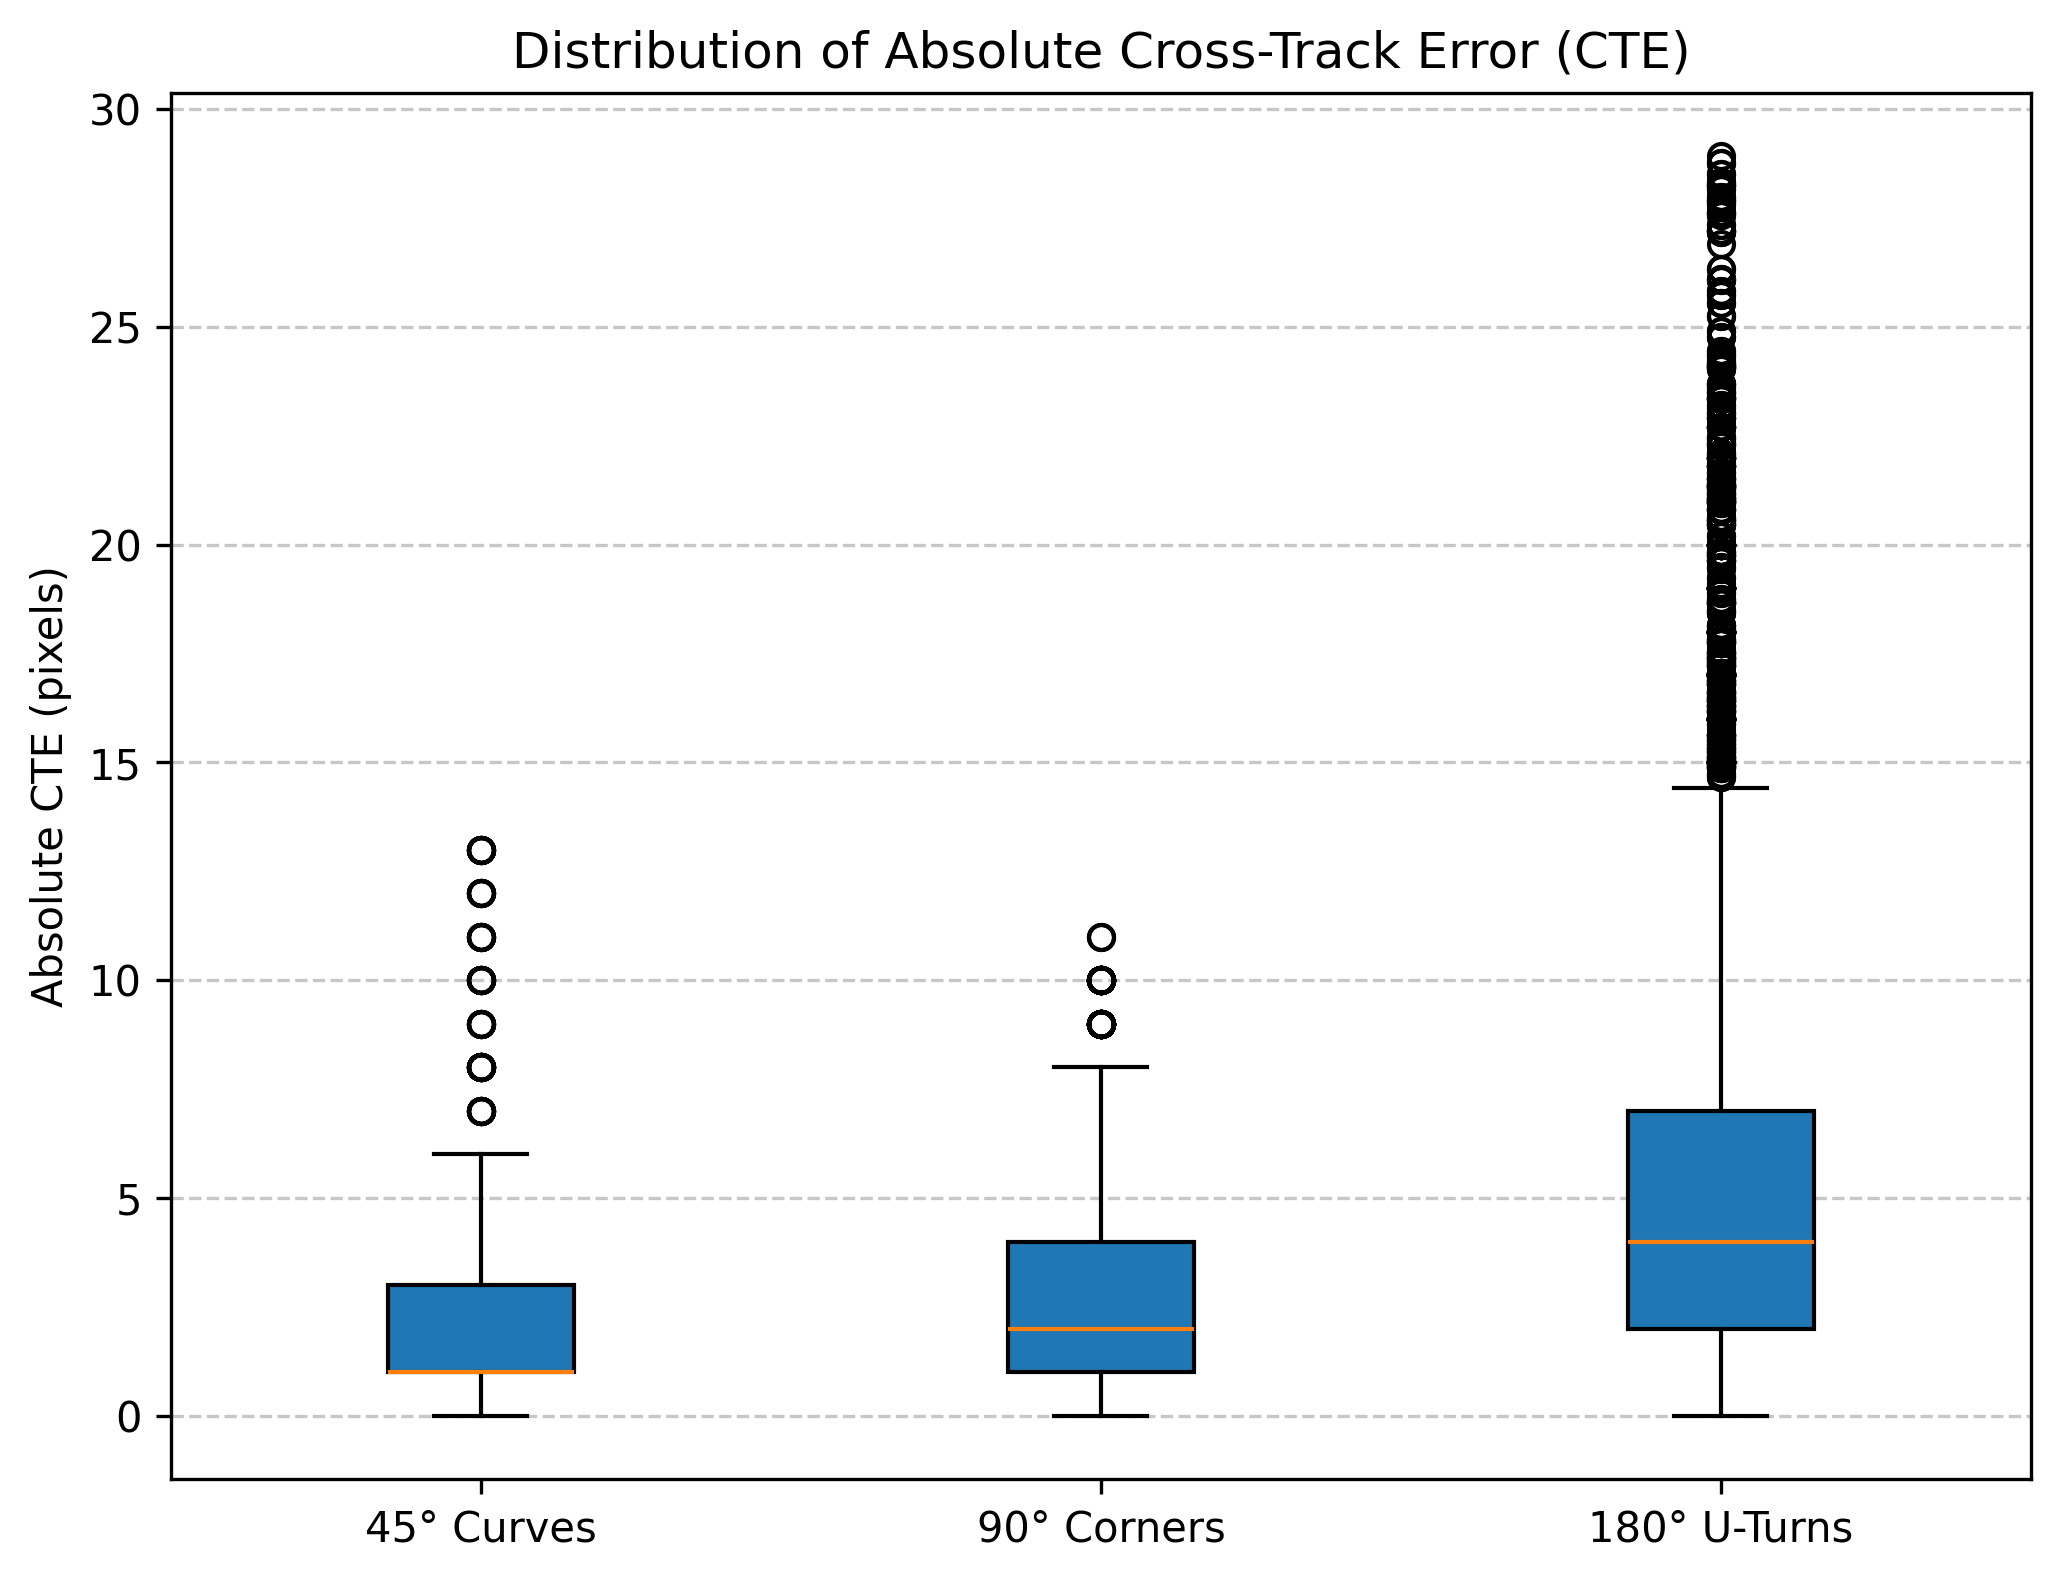
\includegraphics[width=1.0\linewidth]{chap4/images/CTE_Boxplot.png}
	\caption{Distribution of Absolute Cross-Track Error (CTE) across varying B{\'e}zier curve complexities, demonstrating bounded error scaling under extreme geometric distortion.}\label{fig:4.10}
\end{figure}

\section{Control Decision Discretization and Confusion Matrix}
To evaluate the directional correctness of steering decisions issued by the end-to-end CNN, the continuous telemetry logs were mapped to discrete control states. Under the system's sign convention, positive values denote rightward sense for both quantities: a positive CTE indicates the robot is displaced to the \emph{right} of the reference path, and a positive steering command drives a rightward turn. Consequently, a positive CTE calls for a corrective \emph{leftward} steering action. The desired corrective action is therefore defined from the lateral displacement (CTE) as:

\begin{equation}
\text{Desired Action} =
\begin{cases}
\text{Left}, & \text{if } \text{CTE} > 2.0\text{ px} \\
\text{Straight}, & \text{if } -2.0\text{ px} \le \text{CTE} \le 2.0\text{ px} \\
\text{Right}, & \text{if } \text{CTE} < -2.0\text{ px}
\end{cases}
\end{equation}

The executed CNN control action is discretized from the raw steering command using the same $\pm 2.0$ dead-band, with commands greater than $+2.0$ classified as Right, those below $-2.0$ as Left, and those in between as Straight. With this convention, the matrix diagonal corresponds to correct corrective steering. The combined confusion matrix across all three track topologies is shown in Figure~\ref{fig:4.11}.

\begin{figure}[H]
	\centering
	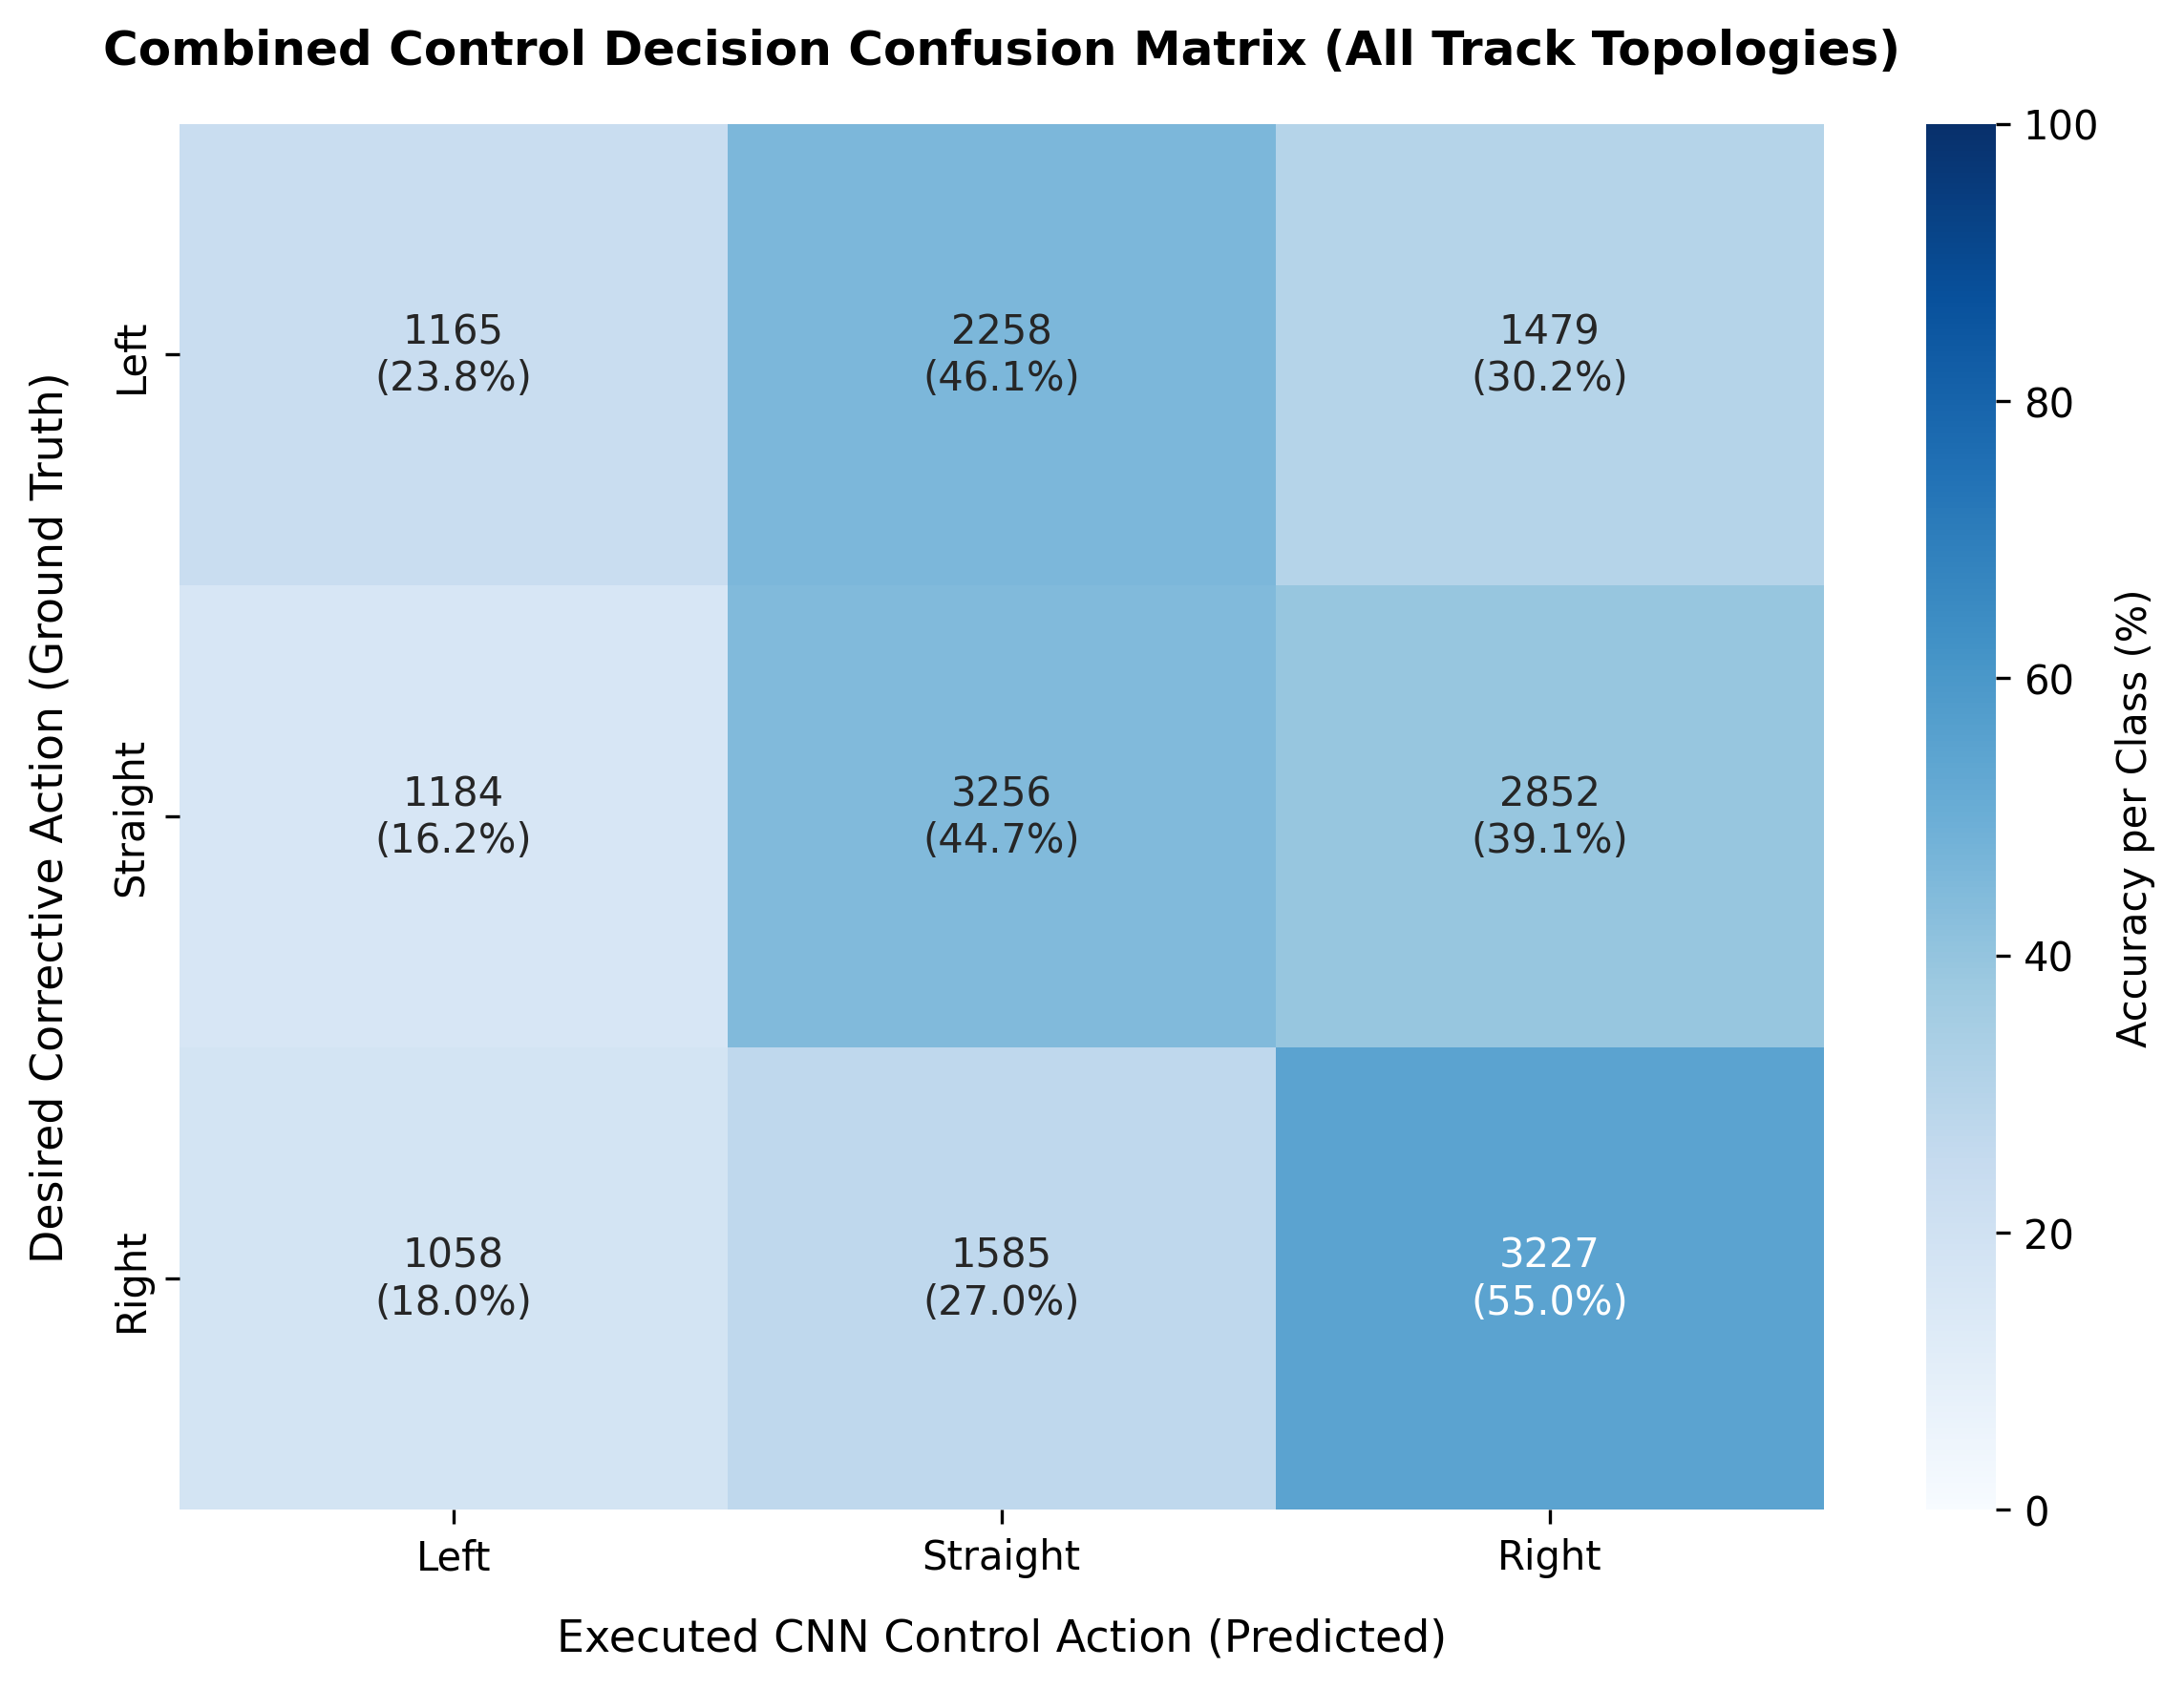
\includegraphics[width=0.82\linewidth]{chap4/images/confusion_matrix_combined.png}
	\caption{Combined Control Decision Confusion Matrix across all track topologies. The matrix maps cross-track error states to the corresponding steering actions.}\label{fig:4.11}
\end{figure}

A key control-theoretic observation is the \textit{Proactive Curve-Following Paradox}. When tracking a curve accurately, the controller holds the vehicle near the centerline (ground truth classified as Straight) while still executing active left or right steering to follow the upcoming geometry. The resulting label mismatch does not indicate failure; it demonstrates anticipatory, feedforward trajectory planning rather than a purely reactive corrective policy.
    \chapter{Conclusions and Recommendations}

\section{Summary of Findings}

This study developed and evaluated a lightweight, end-to-end autonomous navigation framework for a differential-drive robot operating in a structured indoor environment. The system replaced traditional sensor-heavy approaches such as LiDAR-based SLAM and multi-sensor fusion with a single overhead RGB camera and four ArUco fiducial markers. A planar homography matrix was dynamically computed at runtime to transform the angled camera feed into a geometrically rectified Bird's-Eye View (BEV) representation of the arena. A modernized DAVE-2 Convolutional Neural Network (CNN), trained exclusively through Behavioral Cloning on human-demonstrated steering data, then mapped this preprocessed visual state directly to continuous steering commands without any intermediate PID feedback or classical planning algorithm.

Physical deployment initially revealed a critical failure mode: the allocentric (full-AOI) state representation caused the network to rely on the robot's absolute pixel position rather than learn generalizable path-following features. This behavior is consistent with shortcut learning, where a model exploits an easy but unintended predictive feature that performs well under training conditions yet fails to generalize under more challenging or real-world conditions. This issue was mitigated through an architectural pivot to an egocentric perception model, wherein the CNN received only a robot-centered crop drawn on a semantically abstracted black canvas. This information bottleneck forced the convolutional layers to learn translation-invariant relative geometric features.

The resulting egocentric model successfully navigated the 45-degree B\'ezier, 90-degree square, and 180-degree U-turn topologies, as well as a held-out track never seen during training, demonstrating that homography-based preprocessing combined with a strict visual information bottleneck can substantially bridge the gap between offline training loss and real-world kinematic performance.

\section{Conclusion}

This study conclusively demonstrates that a lightweight end-to-end autonomous navigation framework using homography-based overhead localization over an egocentric semantic state representation approach can achieve reliable autonomous navigation on a resource-constrained robotic platform. The research directly addressed the central problem statement: the absence of an accessible, low-cost autonomous navigation framework that operates exclusively on camera input in a structured planar environment.

The proposed system fulfilled this requirement without resorting to expensive range sensors, probabilistic mapping pipelines, or high-end onboard computing hardware. A central achievement of this work was the successful elimination of classical PID feedback loops from the control architecture. The trained DAVE-2 CNN produced sufficiently smooth and accurate continuous steering outputs to maintain stable path following across all tested track topologies, including geometrically demanding 90-degree turns and hairpin U-turns.

This validates the core hypothesis of end-to-end Behavioral Cloning: that a neural network, given a well-constructed visual state, can implicitly learn a non-linear control mapping in place of an explicit feedback controller. No classical PID or pure-pursuit comparator was implemented in this study, so this is an architectural rather than a comparative-performance claim. Notably, the learned policy tracked all topologies without the sustained oscillatory steering often anticipated from a feedback law lacking a derivative damping term, suggesting that the CNN learned a temporally coherent steering policy from the expert demonstrations.

Perhaps the most significant and transferable finding of this study is the decisive role of the visual information bottleneck in reducing shortcut learning. The full-AOI allocentric model achieved low validation loss during training yet failed during physical deployment, indicating that the network had learned an unintended decision rule based on absolute spatial position rather than the geometric features required for robust path following. According to Geirhos et al., shortcut learning occurs when a model exploits features that are sufficient for good performance on training and similarly distributed test data but fail under out-of-distribution conditions. The observed failure of the allocentric representation aligns with this behavior, as the learned strategy did not transfer reliably to real-world operating conditions. By replacing this representation with a semantically abstracted robot-centered crop on a black canvas, the representation removed many of the positional cues that enabled shortcut learning. As a result, the network was encouraged to learn features based on relative path geometry rather than absolute arena position, leading to improved generalization during physical deployment\cite{geirhos2020shortcut}.


This forced the convolutional feature extractor to operate exclusively on relative geometric cues such as the curvature, orientation, and proximity of the approaching path boundaries, which are the only features that generalize across track positions and recovery scenarios. This architectural decision became the definitive factor separating successful real-world deployment from offline training success and represents a replicable design principle for future low-cost end-to-end navigation systems.

More broadly, this study demonstrates that the integration of classical geometric computer vision, specifically projective homography, with modern imitation learning is a viable and computationally efficient strategy for structured indoor robot navigation. By offloading the burden of 3D geometry interpretation from the neural network to a deterministic analytical transformation, the complexity of the learning task was substantially reduced.

A compact DAVE-2 CNN with approximately 2.2 million parameters (2{,}211{,}175) was sufficient to learn reliable path-following behaviors that would otherwise require much deeper architectures when operating on raw perspective images. The system's successful operation on a laptop-class GPU, with real-time inference delivered over a local wireless link to a low-cost microcontroller-driven robot, further confirms the feasibility of this approach for educational and resource-constrained industrial applications.

\section{Recommendations for Future Work}

\subsection{Onboard Hardware Acceleration and Latency Reduction}

The current architecture offloads all image processing and CNN inference to a remote workstation, with control commands transmitted to the robot over a local Wi-Fi link. This centralized design introduces network-dependent latency that may become problematic at higher robot velocities or in environments with wireless interference.

Future work should explore migrating the inference pipeline directly onto an onboard edge computing platform. Deploying the trained DAVE-2 model on an NVIDIA Jetson Nano or a Google Coral Edge TPU would eliminate the round-trip network delay and increase the effective control loop frequency beyond the measured operating rate of approximately 30~Hz.

Model compression techniques such as post-training quantization (INT8) and structured pruning should also be evaluated, as the simplified BEV input representation suggests that the network may be substantially over-parameterized for the task.

\subsection{Dynamic Obstacle Integration}

A fundamental limitation of the current Behavioral Cloning approach is its inability to safely handle dynamic obstacles. The training dataset captures human driving in a static environment, and the learned policy has no mechanism for detecting or responding to objects that appear unexpectedly on the track.

Future iterations should investigate integrating the existing vision pipeline with lightweight secondary sensing modalities. Ultrasonic rangefinders or miniature 1D LiDAR sensors mounted on the robot chassis could provide a proximity signal that triggers a rule-based stop or yield behavior operating independently of the CNN controller.

Alternatively, a lightweight object detection module such as MobileNet-SSD running in parallel on the overhead frame could inject obstacle presence as an additional channel in the state representation, allowing the CNN to learn obstacle-aware steering policies through augmented data collection sessions.

\subsection{Arena Scaling and Marker-Free Generalization}

The current system is constrained to a predefined arena bounded by four fixed ArUco corner markers, limiting its operational area to approximately one square meter in the prototype implementation.

Future work should investigate scaling the homography framework to larger environments through distributed marker networks or the use of higher-resolution cameras with wider fields of view. A more ambitious extension would explore replacing the fiducial-marker homography system with a learned monocular depth estimation module capable of generating approximate BEV representations in environments where physical marker installation is impractical.

\subsection{Dataset Augmentation and Robustness to Illumination Variation}

The trained model is sensitive to environmental conditions that affect ArUco marker detectability, particularly inconsistent or low-contrast lighting. Because the current training dataset was collected under controlled artificial lighting conditions, the learned policy is not robust to detection failures caused by natural light variation, specular reflections, or partial marker occlusion.

Future data collection protocols should deliberately include sessions under varied lighting conditions, shadow patterns, and partial marker visibility to improve the robustness of the perception pipeline. Additionally, offline data augmentation strategies such as synthetic brightness and contrast jitter applied to the egocentric crops may improve the CNN's tolerance to minor rendering artifacts without requiring additional physical driving sessions.

\subsection{Recurrent and Attention-Based Architectures}

The current DAVE-2 architecture processes each frame independently as a stateless regression model. This design does not leverage temporal context, such as recent steering history or the observed trajectory of the approaching path over preceding frames.

Integrating a recurrent module such as a Long Short-Term Memory (LSTM) layer appended to the fully connected stack, or a lightweight spatiotemporal attention mechanism, could enable the network to anticipate upcoming curves based on changes in path curvature rather than reacting solely to the instantaneous visual state.

This is particularly relevant for suppressing the residual oscillatory steering behavior observed at higher throttle speeds, where latency in the single-frame control loop becomes a contributing factor to instability.

\section{Final Remarks}

This research demonstrates that reliable autonomous navigation can be achieved using a minimal and low-cost vision-based framework when classical geometric transformations are effectively combined with modern imitation learning techniques. The study highlights the importance of carefully designing the robot's visual state representation, particularly in mitigating overfitting and improving sim-to-real transfer performance.

By leveraging homography-based overhead localization and an egocentric semantic perception pipeline, the proposed system achieved stable real-world navigation without relying on expensive sensing hardware or computationally intensive mapping algorithms. The findings of this study contribute toward the development of accessible and scalable autonomous robotic systems suitable for educational, research, and resource-constrained deployment scenarios.

    
\backmatter
    % Bibliography
    \if@openright\cleardoublepage\else\clearpage\fi
    \bibliographystyle{plainnat} %% specific plainnat does not show url for articles
    {\footnotesize\bibliography{bibliography}}
	\printindex
	
\appendix
        \chapter{Calendar of Activities}

\begin{table}[h]
\centering
\caption{Project Implementation Schedule and Timeline}
\label{tab:project_schedule}
\resizebox{0.9\linewidth}{!}{% scale to 90% of text width
\renewcommand{\arraystretch}{1.1}%
\begin{tabularx}{\textwidth}{@{} l X l @{}}
\toprule
\textbf{Phase} & \textbf{Activity} & \textbf{Timeline} \\
\midrule
\multicolumn{3}{@{}l}{\textbf{I. Hardware Setup}} \\
& Hardware \& system configuration & Jan Week 1--2 \\
& Chassis assembly \& wiring        & Jan Week 2--3 \\
& Camera mounting \& calibration    & Jan Week 2--3 \\
\addlinespace
\multicolumn{3}{@{}l}{\textbf{II. Software Development}} \\
& OS \& environment setup           & Jan Week 3--4 \\
& Dev: perception (homography)      & Jan Week 4--Feb Week 6 \\
& Dev: data logger module           & Feb Week 6--7 \\
\addlinespace
\multicolumn{3}{@{}l}{\textbf{III. Data Pipeline}} \\
& Dataset collection (driving)      & Feb Week 7--Mar Week 9 \\
& Data cleaning \& augmentation     & Mar Week 10--11 \\
\addlinespace
\multicolumn{3}{@{}l}{\textbf{IV. Model Development}} \\
& CNN architecture design \& dev.   & Mar Week 12--13 \\
& Model training (GPU)              & Apr Week 13--14 \\
& Hyperparameter tuning             & Apr Week 14--15 \\
\addlinespace
\multicolumn{3}{@{}l}{\textbf{V. Integration \& Testing}} \\
& Deployment to robot               & May Week 14--15 \\
& Scenario testing (A, B, C)        & May Week 15--17 \\
& Analysis \& documentation         & May Week 17 \\
\bottomrule
\end{tabularx}
}% end resizebox
\end{table}
     % these are just test names as I didn't know what you'd
        \chapter{Personal Vitae}
John Christian Niño T. Abuel
\begin{itemize}
    \item Title: 4th Year Bachelor of Science in Computer Science
    \item Affiliation: Mindanao State University – Iligan Institute of Technology
    \item Address: Block 2 Lot 27 Doña Maria Subdivision Phase 5, Tipanoy, Iligan City
    \item Contact Number: 0945 702 5852
    \item Email Address: johnchristiannino.abuel@g.msuiit.edu.ph
\end{itemize}

Kervin Lemuel Paalisbo
\begin{itemize}
    \item Title: 4th Year Bachelor of Science in Computer Science
    \item Affiliation: Mindanao State University – Iligan Institute of Technology
    \item Address: Poblacion Linamon Purok 5-A, Lanao Del Norte
    \item Contact Number: 09924779137
    \item Email Address: kervinlemuel26@gmail.com
\end{itemize}
Rey Iann Tigley 
\begin{itemize}
    \item Title: 4th Year Bachelor of Science in Computer Science
    \item Affiliation: Mindanao State University – Iligan Institute of Technology
    \item Address:  Prk Sudlonon, San Miguel, Iligan City, 9200 Lanao del Norte
    \item Contact Number: 09605052173
    \item Email Address: reyiann.tigley@g.msuiit.edu.ph
\end{itemize}


\end{document}

%%% The End %%%
